\chapter{Calorimeter Optimisation Studies}
\label{chap:detopt}

\chapterquote{The simple believes everything, but the prudent gives thought to his steps.}
{Proverbs 14:15}

%========================================================================================
%========================================================================================

\section{Introduction}
\label{sec:optimisationstudies}
The fundamental principle of particle flow calorimetry is to measure the energy of a particle passing through a detector in whichever sub-detector offers the best energy resolution.  For particle collider experiments, this involves measuring the momenta of charged particles using the curvature of the track they create in the detector.  This offers extremely good energy resolution in comparison to calorimetric energy measurements and is the source of the excellent energy resolution that particle flow calorimetry can produce.  As neutral particles produce no tracks, their energies must be measured using calorimetric energy deposits.  

The application of particle flow calorimetry is extremely challenging as it is possible, by using incorrect associations of charged particle tracks to calorimetric energy deposits, to both double count and omit energy measurements.  For example:
\begin{itemize}
\item If part of the calorimetric energy deposit from a charged particle is not associated to the track that energy deposit is double counted.
\item If part of the calorimetric energy deposit from a neutral particle is incorrectly associated to a track, the energy deposit is not accounted for.
\end{itemize}
\noindent These effects, collectively know as "confusion", degrade the energy resolution of a particle flow detector.  Therefore, it it is crucial to make correct associations between charged particle tracks and calorimetric energy deposits to minimise the effect of confusion.  These associations can only be successfully made if the calorimeters in use have fine segmentation, such as those found at the linear collider experiment, so that it becomes possible to separate the energy deposits from nearby showering particles.  Even with this segmentation, making the association of charged particle tracks to the calorimetric energy deposits is highly non-trivial.  At the linear collider experiment, these associations are made using sophisticated pattern recognition algorithms, provided by PandoraPFA.  The fine segmentation of the calorimeters allows PandoraPFA to reconstruct the four-momenta of all particles passing through the detector and to use the energy measurement from the optimal sub-detector in each case. 

This chapter considered optimisation of the calorimeters used at the linear collider, with focus placed on obtaining the best energy resolution for jets.  Parameters such as the number of layers, cell size and material choices for the calorimeters are investigated.  This chapter concludes with an optimisation of several global parameters for the detector such as the magnetic field strength used for the detector and the inner radius of the ECal.  These parameters are not calorimeter specific, but affect the jet energy resolution obtained from particle flow. 

%========================================================================================
%========================================================================================

\section{Jet Energy Resolution}
\label{sec:optstudiesmetric}
As many physics processes of interest at the linear collider involve multi-jet final states, good jet energy resolution is a crucial a aspect of detector performance.  As shown in chapter \ref{chap:PhysicsAnalysis}, parameters derived from the energy measurements of jets, such as invariant mass, are extremely useful for identification of physics channels of interest as well as determining the sensitivity of the linear collider experiments to areas of new physics.  Therefore, the primary metric used in this study is the jet energy resolution.

Jet energy resolution in particular can benefit from the application of particle flow calorimetry as $\approx 70 \%$ of the energy of jets are carried in the form of charged particles.  As particle flow aims to measure the energy of charged particles using the tracker, it has the potential to offer extremely large benefits when measuring jet energies in comparison to the traditional calorimetric approach.  

%========================================================================================

\subsection{Jet Energy Resolution Metrics}
The primary metric used to optimise detector performance is the jet energy resolution.  This was found through the simulation of off-shell mass Z boson events decaying to light quarks (u, d, s).  In these events the Z boson is produced at rest, which means the typical decays form two mono-energetic jets that are produced back to back as shown in figure \ref{fig:500GeVzudsevtdisplay}.  Only events where $|\text{cos}(\theta)| < 0.7$, where $\theta$ is the polar angle of the quarks from the Z decay, are used in the metric calculation to ensure little energy is lost down the beam axis.  Using these events the jet energy resolution is calculated as follows: 
\begin{equation} 
\frac{\text{RMS}_{90}(E_{i})}{\text{Mean}_{90}(E_{i})} = \frac{\text{RMS}_{90}(E_{jj})}{\text{Mean}_{90}(E_{jj})} \times \sqrt{2} \text{ ,}
\end{equation}
\noindent where $E_{jj}$ is the total reconstructed energy.  $\text{Mean}_{90}(E_{jj})$ and $\text{RMS}_{90}(E_{jj})$ are the mean and root mean squared (RMS) of the $E_{jj}$ distribution.  These variables are calculated across the range of $E_{jj}$ with the smallest RMS containing at least 90\% of the data.  

\begin{figure}[h!]
\centering
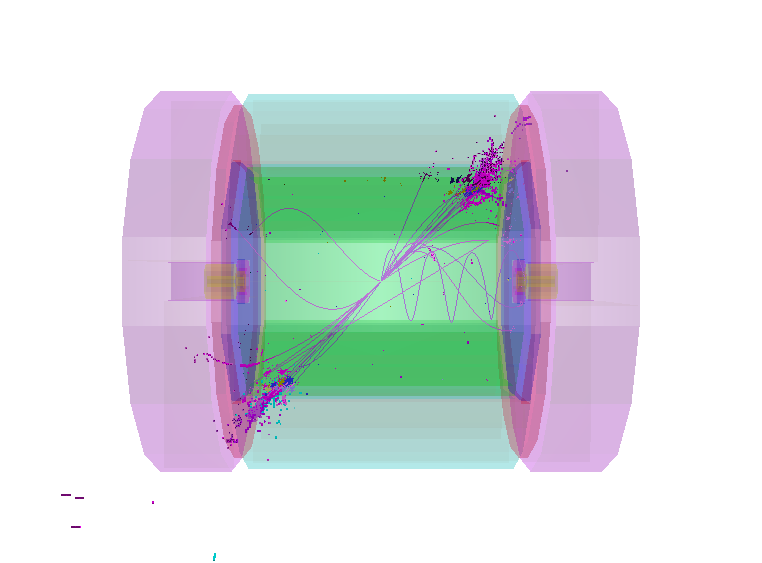
\includegraphics[width=0.75\textwidth]{OptimisationStudies/Plots/MethodDescription/500GeVEvent.png}
\caption[500 GeV di-jet Z$\rightarrow$uds event display for nominal ILD detector.]{500 GeV di-jet Z$\rightarrow$uds event display for nominal ILD detector.}
\label{fig:500GeVzudsevtdisplay}
\end{figure} 

\begin{figure}[h!]
\centering
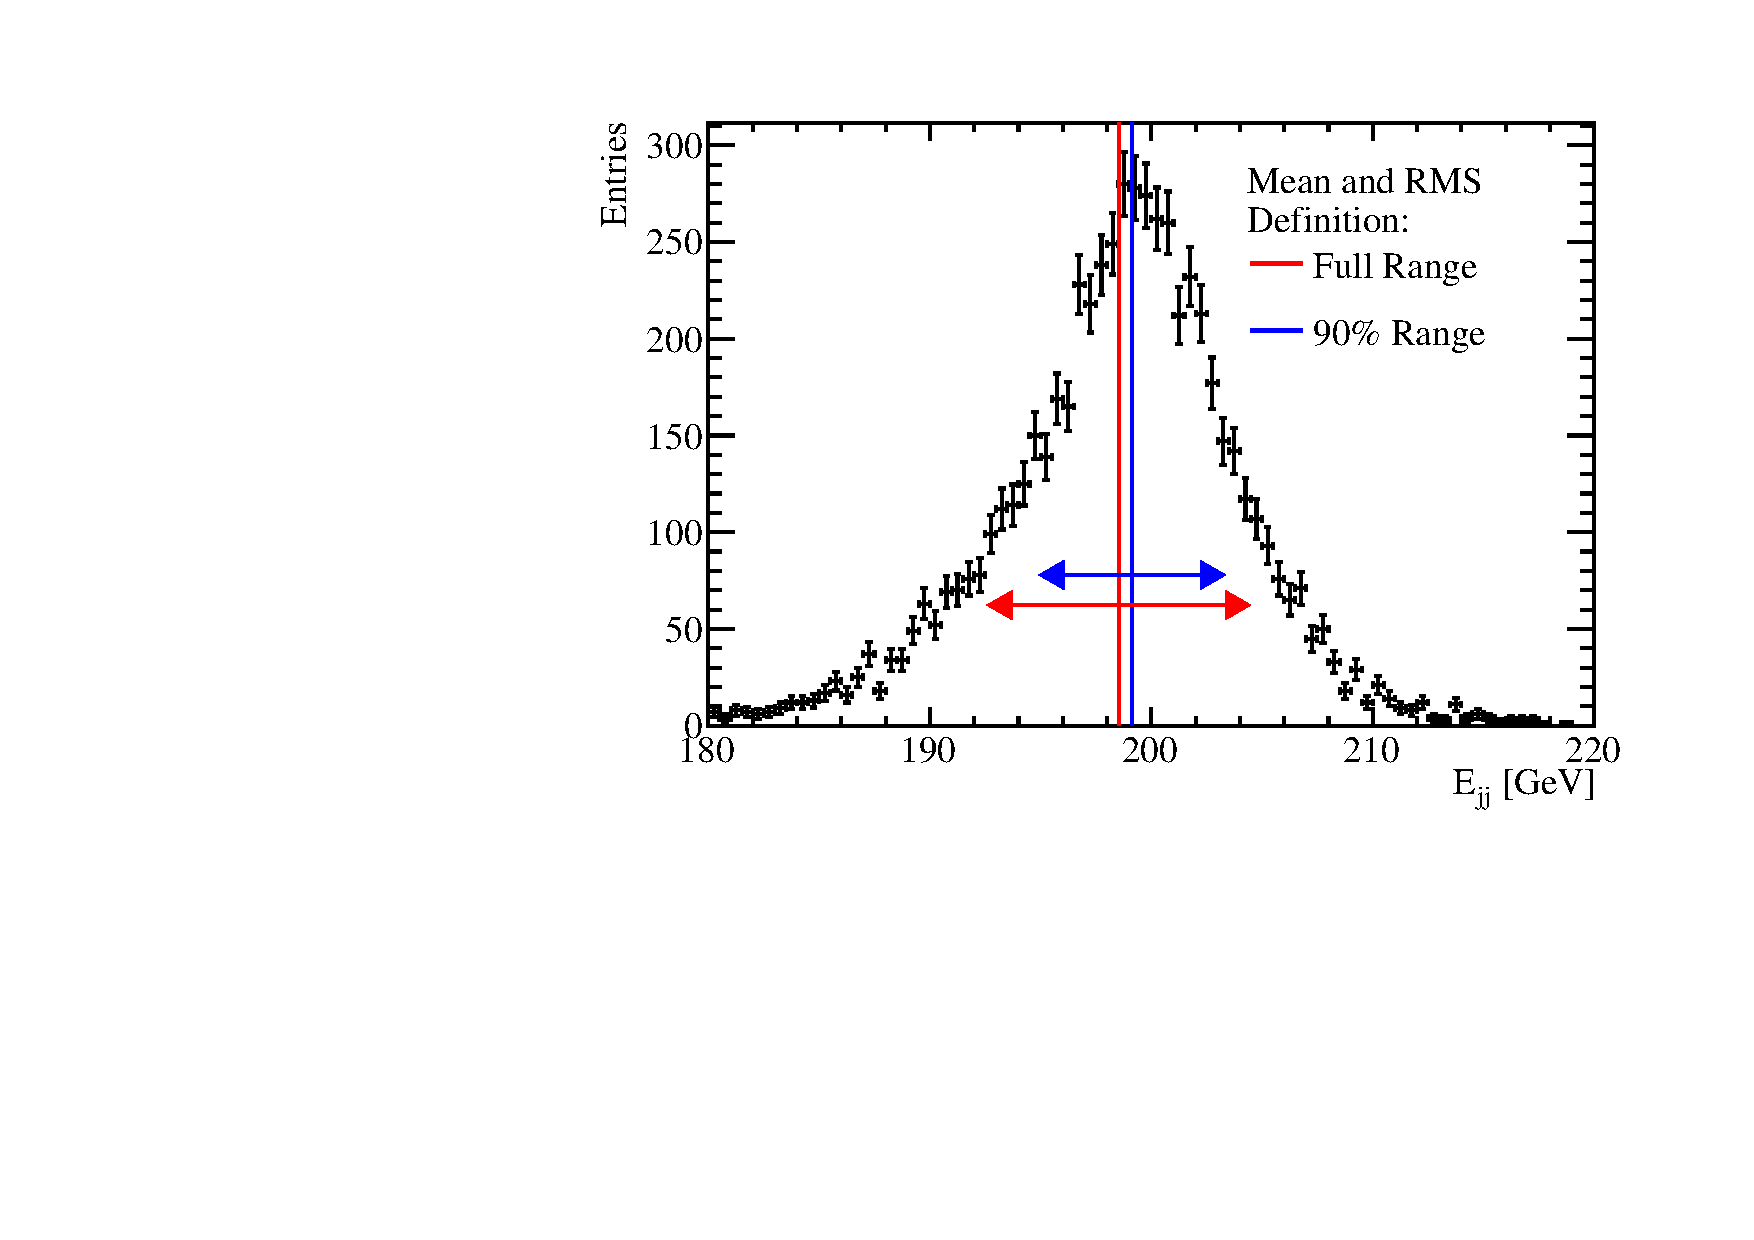
\includegraphics[width=0.5\textwidth]{OptimisationStudies/Plots/MethodDescription/RMS90Plot.pdf}
\caption[Definition of jet energy resolution.   Reconstructed jet energy for 200 GeV di-jet Z$\rightarrow$uds events for nominal ILD detector.]{Definition of jet energy resolution.   Reconstructed jet energy for 200 GeV di-jet Z$\rightarrow$uds events for nominal ILD detector.}
\label{fig:rms90defintion}
\end{figure} 

This definition is used to remove the effect of outliers in the distribution \cite{arXiv:0907.3577}.  Although the correct combination of charged particle tracks and calorimetric energy measurements would give a Gaussian reconstructed jet energy distribution, the effect of confusion on certain events will distort this distribution and broaden the tails significantly.  If the full range were to be used in the jet energy resolution calculation, the effect of these tails is overinflated.  If the distribution of reconstructed jet energies is truncated to the narrowest range of the data containing at least $90\%$ of the data, the effect of these tails can be negated.  This removes events where confusion is dominant, which makes the jet energy resolution metric far more robust and representative of the bulk of the data.  

An example of the application of this metric can be found in figure \ref{fig:rms90defintion}.  The RMS calculated using the full range is 5.8~GeV, while the RMS using the reduced range is 4.1~GeV.  This corresponds to a reduction in the jet energy resolution from $4.1\%$ to $2.9\%$, which clearly shows an overemphasis of the tails of the distribution if the full range is used in the calculation.

In the subsequent analysis a range of di-jet energies were considered ranging from the Z mass, 91~GeV, to the nominal running energy of the ILC, 500~GeV.  Each event sample contained 10,000 events generated isotropically so that, given the polar angle cut, approximately 7,000 events contribute to the jet energy resolution metric. 

%========================================================================================

\subsection{Jet Energy Resolution Decompositions}
It is possible to gain insight into the detector performance by cheating various parts of the pattern recognition using the MC information.  Cheating the pattern recognition removes the effect of confusion as it ensures no errors are made when either clustering calorimeter hits together or when associating charged particle tracks to those calorimeter clusters.  This allows the detector performance to be deconstructed into two terms; one related exclusively to the intrinsic energy resolution of the detector and another related to the pattern recognition confusion.  The additional information this provides is extremely useful for characterising changes to the overall detector performance.  

The intrinsic energy resolution contribution to the jet energy resolution is determined by fully cheating the pattern recognition; in this case all confusion is negated.  The total confusion is defined as the quadrature difference between the jet energy resolution using the standard reconstruction and this fully cheated reconstruction.  Furthermore, it is possible to cheat the pattern recognition associated with individual types of particles.  This is particularly useful for studies related to the ECal as, by cheating the photon pattern recognition, it is possible to isolate the confusion associated with photons.  The photon confusion is defined as the quadrature difference between the jet energy resolution using the standard reconstruction and the reconstruction where photons pattern recognition is cheated.    

%========================================================================================

\subsection{Single Particle Energy Resolution}
Several physics studies rely on the identification of single particles, such as $\gamma$ in anomalous triple gauge coupling studies CITE, and as such the energy resolution of individual particles is presented alongside the jet energy resolution metric.  As only uncharged particle energies are measured in the calorimeters in the particle flow paradigm, the single particle energy resolution is shown using $\gamma$s and $K^{0}_{L}$s.  $\gamma$s are particularly relevant for several physics studies and, as they are largely contained within the ECal, they provide insight into detector changes related purely to the ECal.  This makes $\gamma$s a natural choice of particle to consider for this study.  $K^{0}_{L}$s were used as, analogously to $\gamma$s and the ECal, their energies are primarily measured using the HCal.  Although in general neutral hadron energy resolutions are less crucial to physics studies, the energy resolution is still a crucial contribution to the jet energy resolution, which should not be overlooked.  For these single particle samples the energy resolution is defined using a Gaussian fit to the reconstructed energy distributions.  The fit was applied to the narrowest region of the reconstructed PFO energy distribution that contained at least 75\% of the data.  This increases the likelihood that the fit converges and ensures a better parameterisation of the bulk of the data set.  The resolution is defined as the standard deviation divided by the mean of that reconstructed Gaussian.  A total of 10,000 events are used to calculate the energy resolution at each fixed energy point.  A cut of $|\text{cos}(\theta)| < 0.7$ is applied to ensure events avoid the Barrel/EndCap overlap region.  Examples of the single particle energy distributions for 100 GeV $\gamma$s and 50 GeV $K^{0}_{L}$s alongside the Gaussian fit used to determine their energy resolution are shown in figure \ref{fig:singleparticleenergyhists}.  The errors quoted on single particle energy resolutions are determined by propagating the errors reported from the Gaussian fit into the resolution calculation.  

\begin{figure}[h!]
\centering
\subfloat[50 GeV $K^{0}_{L}$.]{\label{fig:kaonsingleparticleenergyhist}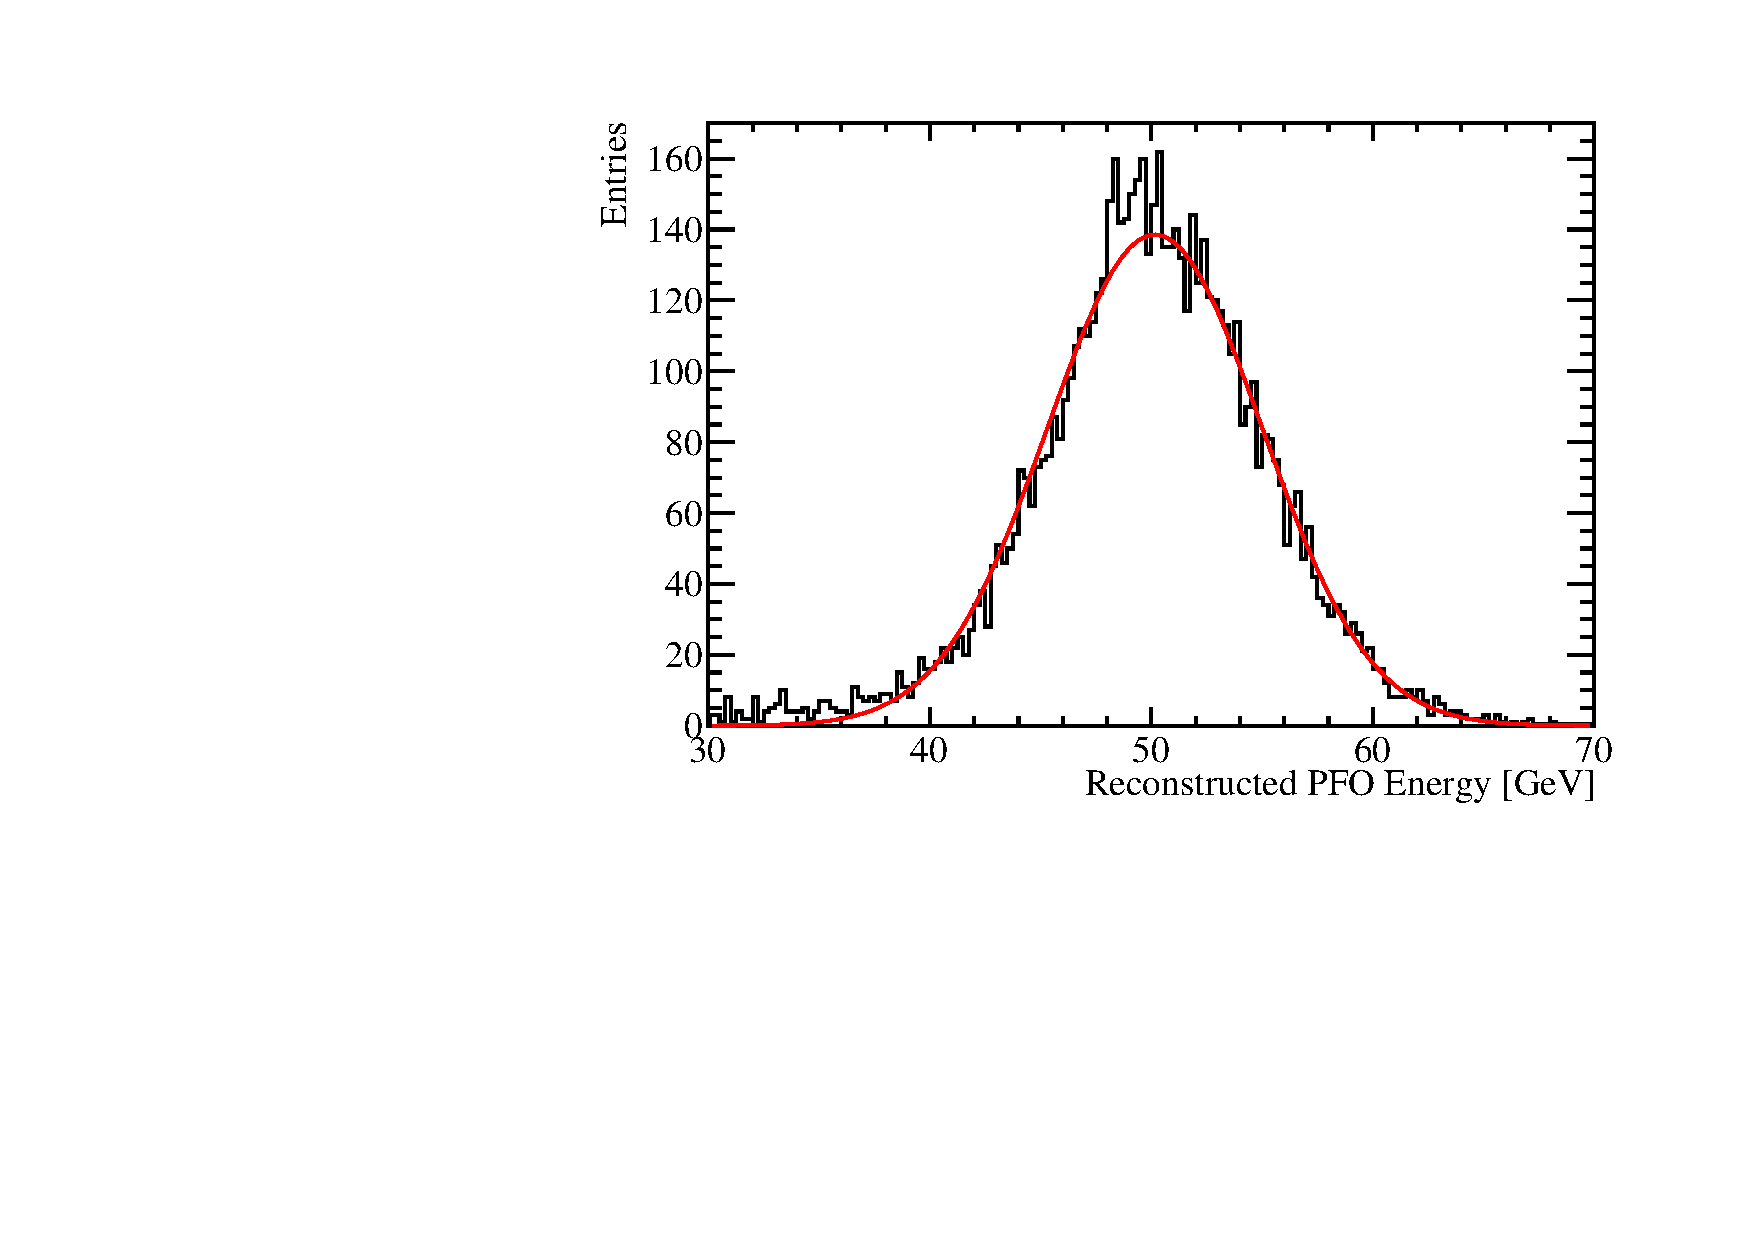
\includegraphics[width=0.5\textwidth]{OptimisationStudies/Plots/EnergyResolution/EKaon0L_50GeV.pdf}}
\subfloat[100 GeV $\gamma$.]{\label{fig:photonsingleparticleenergyhist}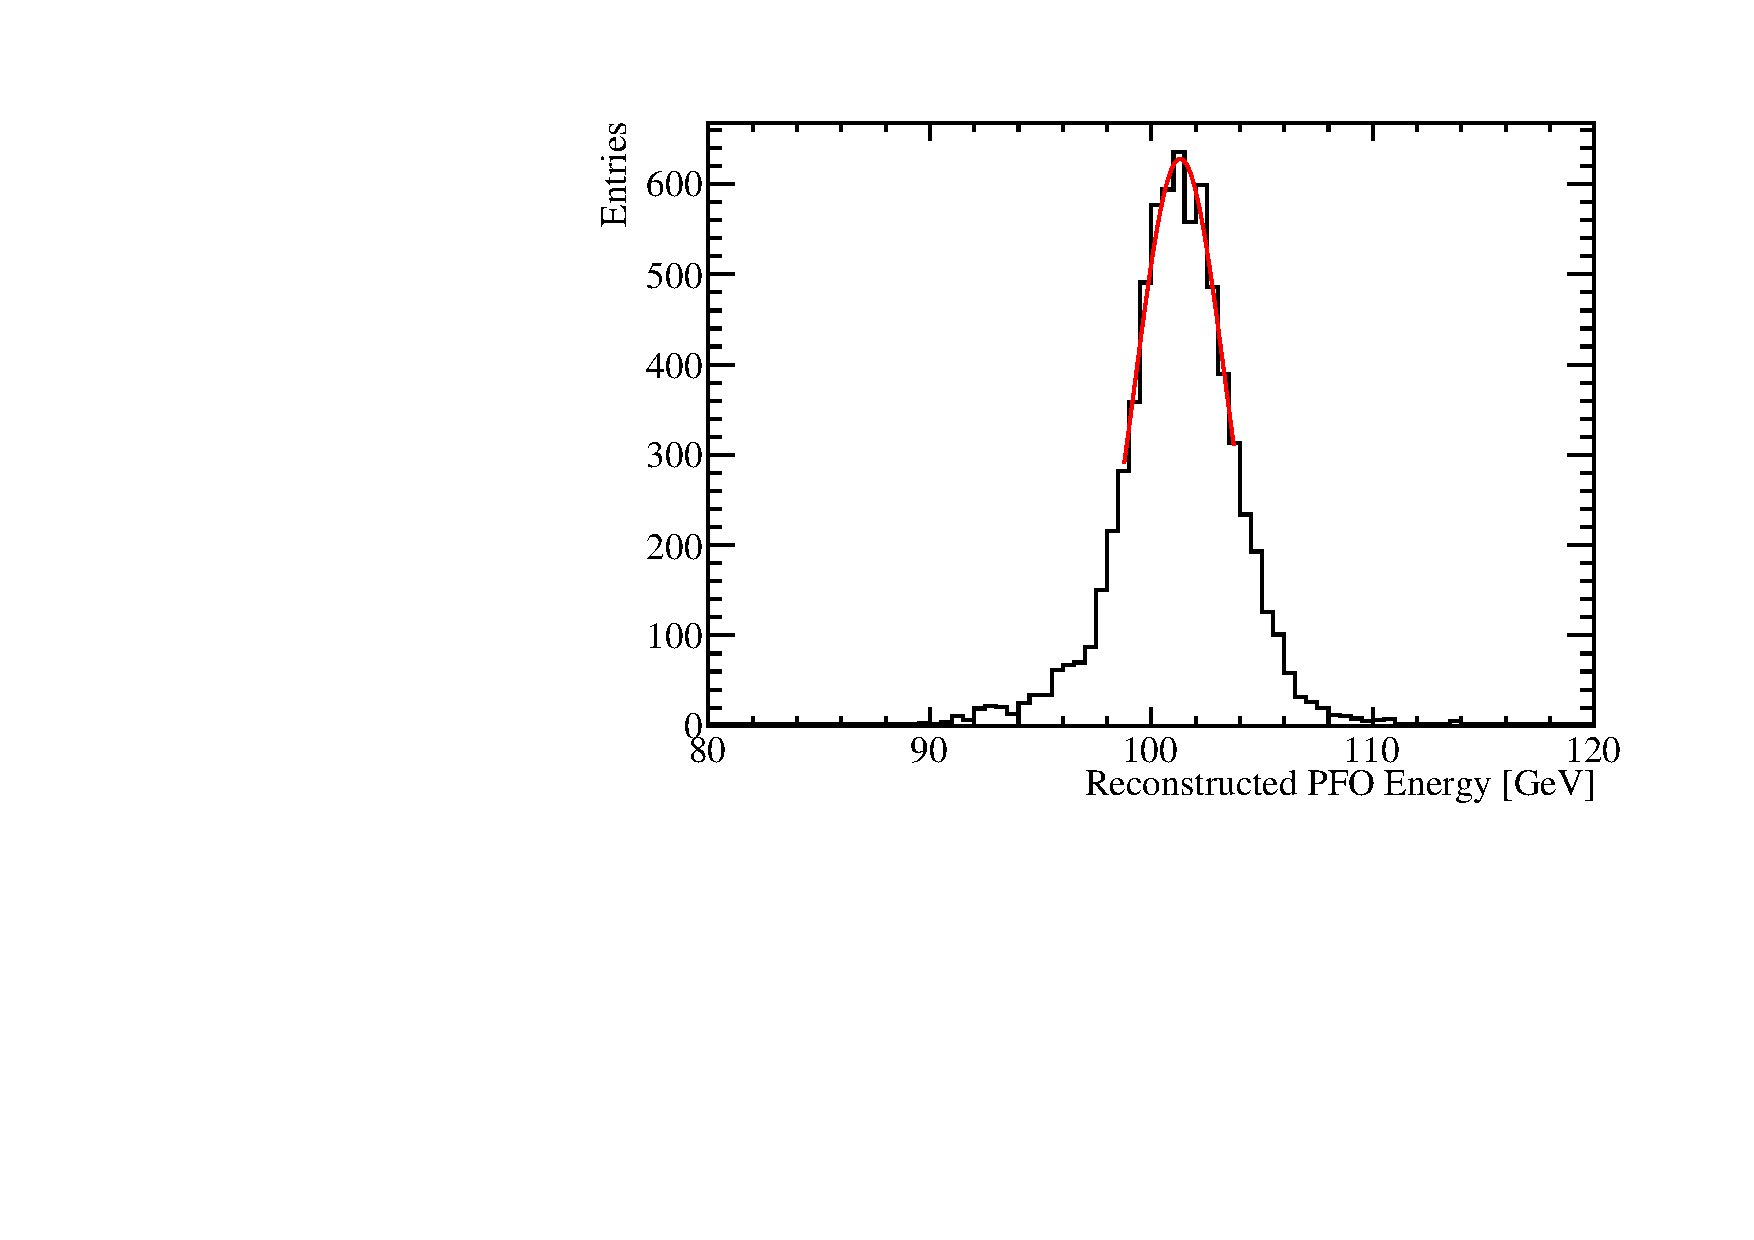
\includegraphics[width=0.5\textwidth]{OptimisationStudies/Plots/EnergyResolution/EPhoton_100GeV.pdf}}
\caption[The reconstructed energy distribution for \protect\subref{fig:kaonsingleparticleenergyhist} 50 GeV $K^{0}_{L}$ and \protect\subref{fig:photonsingleparticleenergyhist} 100 GeV $\gamma$ events.  The red line shows a Gaussian fit used to parameterise the detector performance.  The fit was applied to the truncated range of the reconstructed PFO energy distribution containing at least 75\% of the data with the narrowest RMS.  The nominal ILD model was used in this simulation.]{The reconstructed energy distribution for \protect\subref{fig:kaonsingleparticleenergyhist} 50 GeV $K^{0}_{L}$ and \protect\subref{fig:photonsingleparticleenergyhist} 100 GeV $\gamma$ events.  The red line shows a Gaussian fit used to parameterise the detector performance.  The fit was applied to the truncated range of the reconstructed PFO energy distribution containing at least 75\% of the data with the narrowest RMS.  The nominal ILD model was used in this simulation.}
\label{fig:singleparticleenergyhists}
\end{figure}

%========================================================================================
%========================================================================================

\section{Nominal Detector Performance}
\label{sec:nominaldetectorperformance}
Before addressing the optimisation of the detectors for use at a future linear collider it is necessary to properly quantify the behaviour of the nominal detector model that is used in the simulations.  For these studies the nominal ILD model is used.  

The calorimeters at a linear collider are sampling calorimeters, therefore, the reconstructed energy distributions for neutral particles whose energies are measured in the calorimeters will be Gaussian.  This is expected as the active material for each calorimeter cell essentially counts the number of charged particle tracks passing through it, or possible the number of photons for scintillator options.  An estimation of the total energy deposited in the calorimeter cell, including the absorber material, can be made based upon this number of tracks or photons.  For more details on how this estimation is made see chapter \ref{sec:calibration}.  Finally, the energy of the entire particle shower is estimated by grouping together calorimeter cells and summing their energy.  Each calorimeter cell energy is an independent random measurement and, by the central limit theorem, their sum has a Gaussian distribution.  Furthermore, it follows that the variance of the shower energy distribution is given by the sum of the variances for each of the calorimeter cell energy distributions.  

As each calorimeter hit involves counting a number of objects, charged particle tracks or photons, the statistics governing the distribution of the individual cell energies are Poisson statistics.  For a given particle shower, if the mean of a cell energy is given by $\lambda = N$ where $N$ is the mean number of objects that are expected, the standard deviation of that distribution is $\sigma = \sqrt{\lambda} = \sqrt{N}$ and the energy resolution $\frac{\sigma}{\lambda} = \frac{1}{\sqrt{N}}$.  As the total shower energy, $E_{Reco}$, is proportional to $N_{Reco}$, the total number of tracks recorded in the calorimeter, the energy resolution for an ideal calorimeter is proportional to $\frac{1}{\sqrt{N_{Reco}}} = \frac{1}{\sqrt{E_{Reco}}}$.  This gives the form of the energy resolution as a function of energy for an ideal calorimeter as $\frac{\sigma_{Reco}}{E_{Reco}} = \frac{a}{\sqrt{E_{Reco}}}$.  In reality, it is typical to express the energy resolution of a calorimeter in the following form

\begin{equation} 
\frac{\sigma_{Reco}}{E_{Reco}} = \frac{a}{\sqrt{E_{Reco}}} \oplus b \oplus \frac{c}{E_{Reco}}\text{ ,}
\end{equation}

\noindent where the $b$ term is a constant term that accounts for a variety of effects such as CHECK and the $c$ term accounts for electrical noise.

Prototypes of the various ILD calorimeter options have been constructed and validated using test beam measurements.  The energy resolution measured using the test beam was parameterised as $\frac{16.6}{\sqrt{E_{Reco}}} \oplus 1.1 \%$ for the silicon ECal and $\frac{12.9}{\sqrt{E_{Reco}}} \oplus 1.2 \%$ for the scintillator ECal \cite{Behnke:2013lya}.  The electrical noise was deemed sufficiently small that the $c$ term in the parameterisation could be neglected in both cases.  These results were determined using an $\text{e}^{-}$ test beam with energies ranging up to $\approx 40$ GeV.  This parametrisation is compared to the results found using the full ILD detector simulation in figures \ref{fig:ecalsinominalres} and \ref{fig:ecalscnominalres} for the silicon and scintillator ECal options respectively.  The parameterisation of the energy resolution for the silicon ECal option is almost identical to the energy resolution results when using the full ILD simulation.  However, for the scintillator ECal option the parameterisation is significantly better than that observed in the full simulation.  This difference is most likely due to an imperfect implementation of the scintillator ECal within the full detector simulation.  Even with this difference, the $\gamma$ energy resolutions measured using the full ILD simulation are similar for the silicon and scintillator ECal options.  At very high energies, $\approx 500$ GeV, the ECal is no longer sufficient to fully contain the $\gamma$s and so leakage into the HCal leads to a minor degradation the energy resolution for the full simulation.  This accounts for the deviation in the energy resolution between the full ILD simulation and the test beam parameterisation for the silicon ECal option.   

Similarly, the energy resolution using test beam was parameterised as $\frac{57.6}{\sqrt{E_{Reco}}} \oplus 1.6 \%$ for the nominal ILD HCal \cite{Adloff:2012gv}.  A comparison between this test beam parameterisation and the full ILD simulation, using the silicon ECal option, is shown in figure \ref{fig:hcalnominalres}.  The test beam used for this parameterisation used $\pi^{\pm}$s with energies ranging from 10 to 80 GeV.  In the determination of the test beam parameterisation, only showers starting in the HCal were considered whereas all showers were considered in the full ILD simulation.  Negating showers starting in the ECal removes the effect of errors associated with the calibration of ECal for hadronic energy measurements and leads to a better energy resolution for the $K^{0}_{L}$.  The deviation between the test beam parameterisation and the full simulation grows at high $K^{0}_{L}$ energies due to the treatment of energy deposits leaking out of the back of the HCal.  A tail catcher was used in the test beam analysis that had a similar structure to the HCal, but with a much wider average absorber thickness.  Energy deposits in this tail catcher were calibrated in a similar fashion to the HCal giving a very good energy resolution for these energy deposits.  In the full ILD simulation a muon chamber acts as the tail catcher, however, the calibration applied to energy deposits here is less advanced than that applied to the test beam data meaning the energy resolution for these hits will be worse.  Furthermore, energy deposits in the uninstrumented solenoid region of the full ILD simulation are not accounted for.  These missing energy deposits and the simplistic muon chamber calibration are the main causes of the deviation between the test beam parameterisation and the full ILD simulation of the energy resolution for high energy $K^{0}_{L}$s.   

The jet energy resolutions as a function of jet energy using the full ILD simulation are shown in figure \ref{fig:jernominalres}.  Alongside this, the intrinsic energy resolution and confusion contributions to the jet energy resolution are also presented.  The jet energy resolution at low energies is dominated by the intrinsic energy resolution of the detector, while at high energies it is dominated by the effect of confusion.  This is to be expected as the intrinsic energy resolution of the calorimeters is proportional $~\frac{1}{\sqrt{E_{j}}}$ meaning that it will dominate the energy resolution at low energies.  On the other hand, confusion is a measure of how easy it is to group calorimeter hits together into clusters and associate those clusters to charged particle tracks and this effect will grow with increasing jet energy as the event topology becomes more dense.  The total jet energy resolution for the ILD detector are sufficiently small, $\frac{\sigma_{E}}{E} \lesssim 3.8\%$ \cite{Behnke:2013lya, arXiv:0907.3577, Linssen:2012hp},  across the energy range considered to make separation of the hadronic decays of the W and Z bosons possible, which is one of the key requirements for the future linear collider

\begin{figure}[h!]
\centering
\subfloat[]{\label{fig:ecalsinominalres}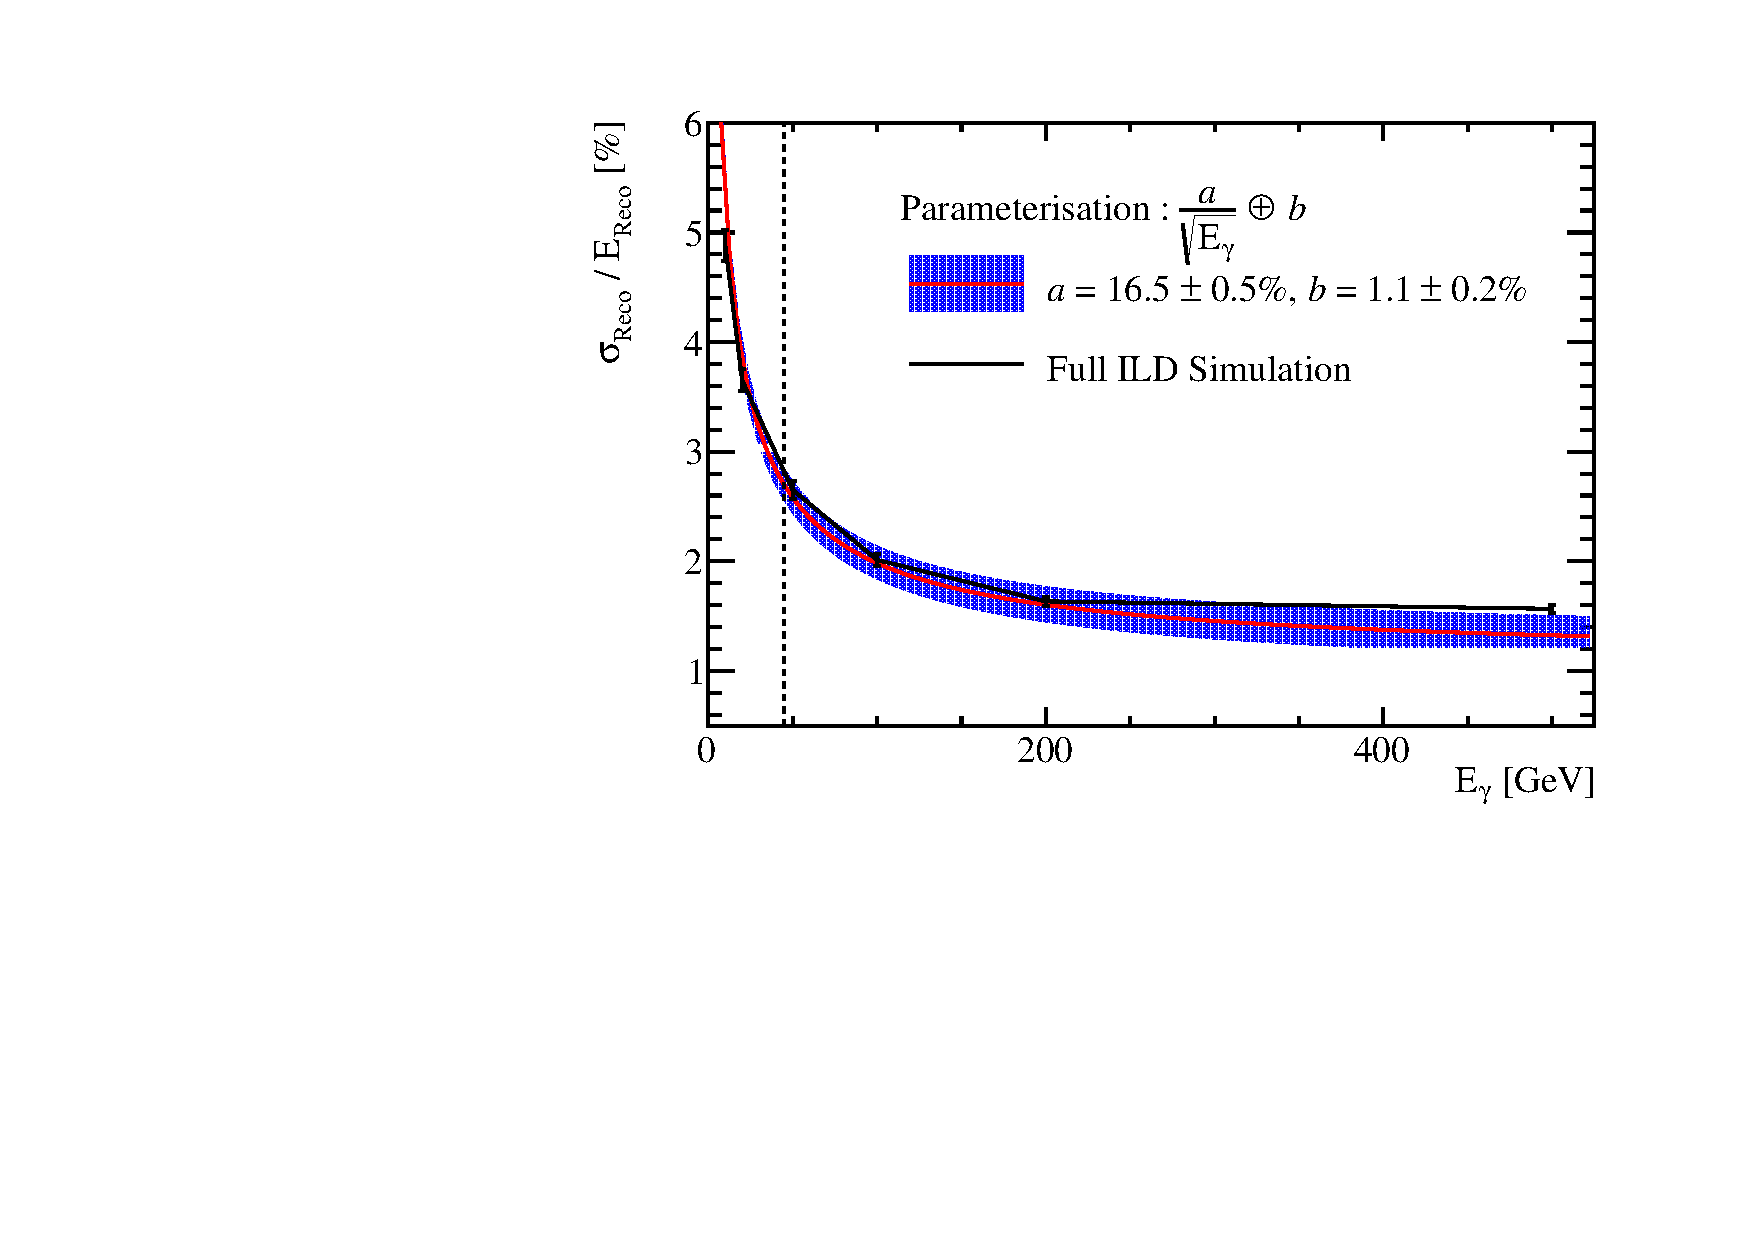
\includegraphics[width=0.5\textwidth]{OptimisationStudies/Plots/EnergyResolution/ER_vs_EGamma_SiECal.pdf}}
\subfloat[]{\label{fig:ecalscnominalres}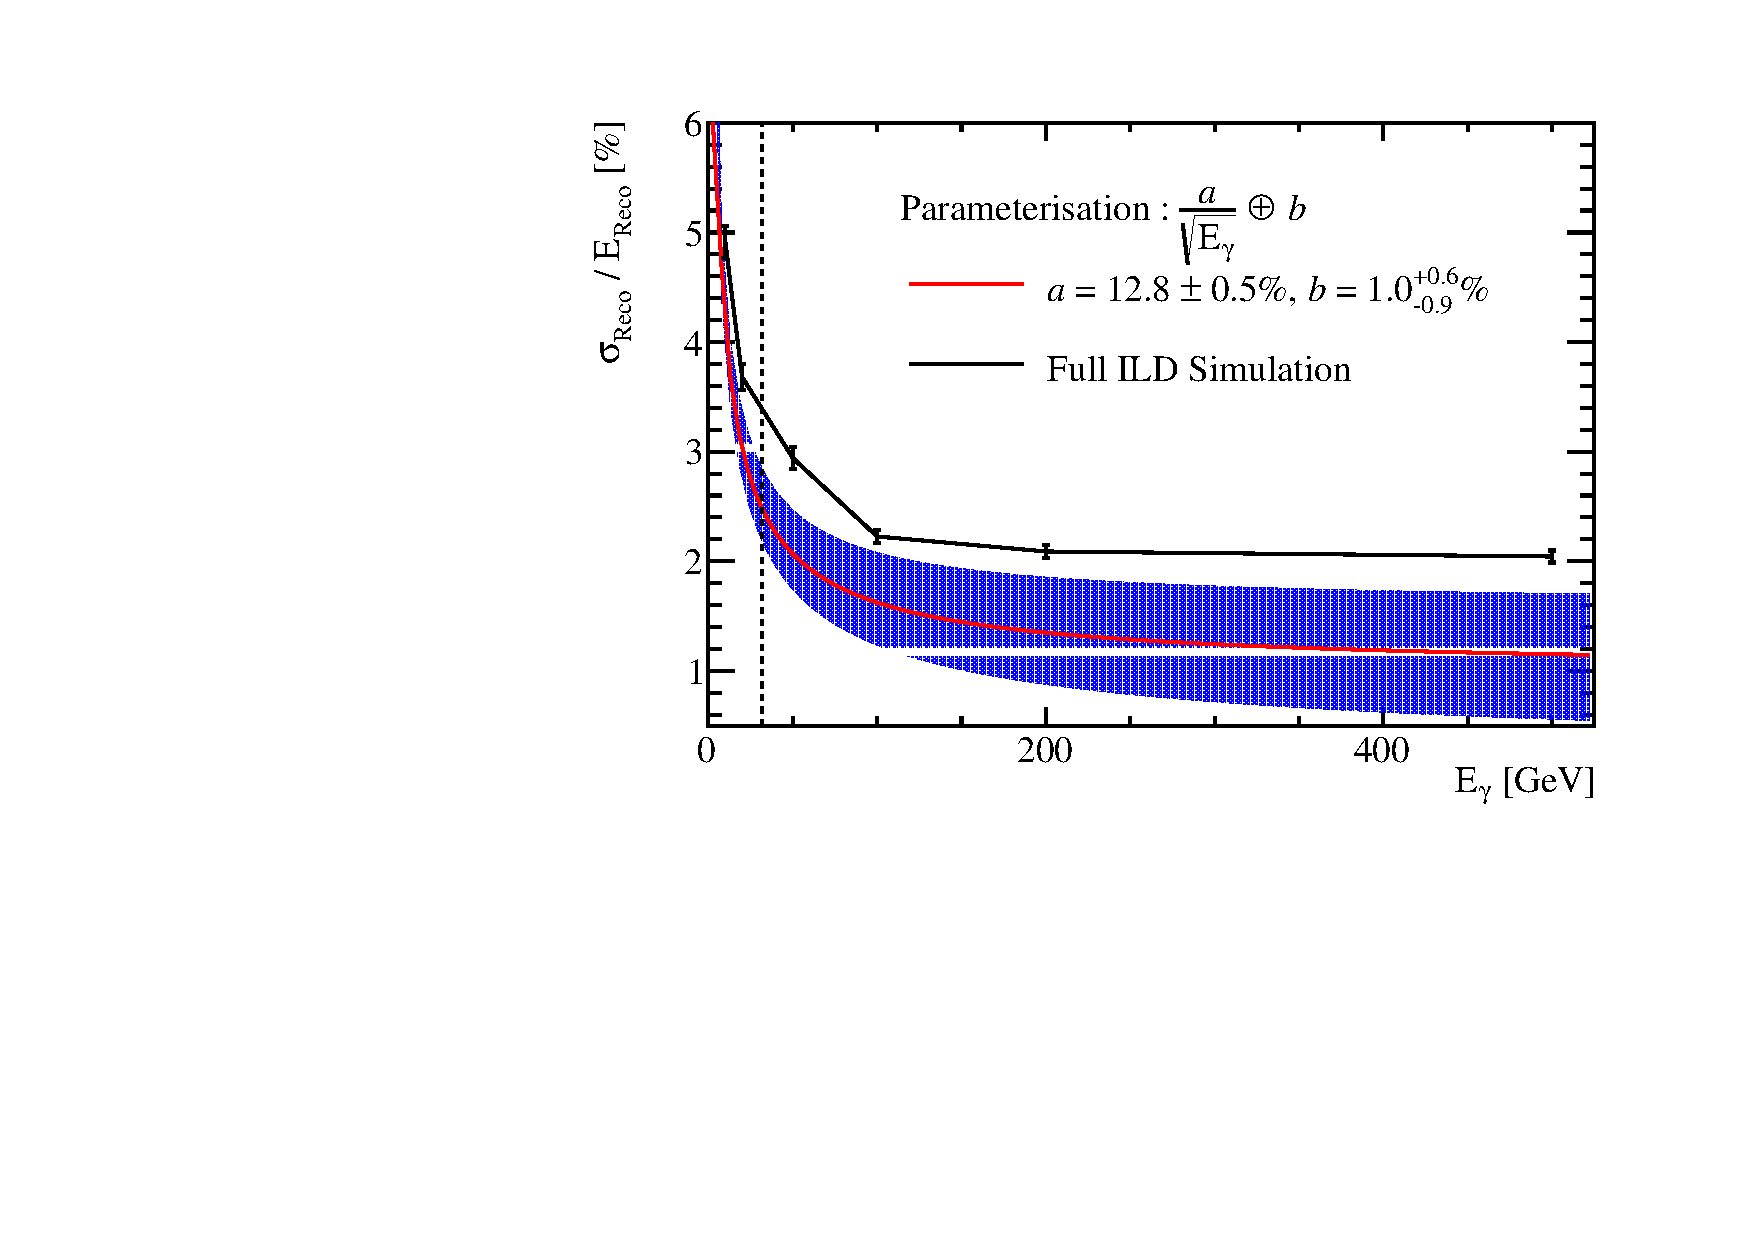
\includegraphics[width=0.5\textwidth]{OptimisationStudies/Plots/EnergyResolution/ER_vs_EGamma_ScECal.pdf}}\\
\subfloat[]{\label{fig:hcalnominalres}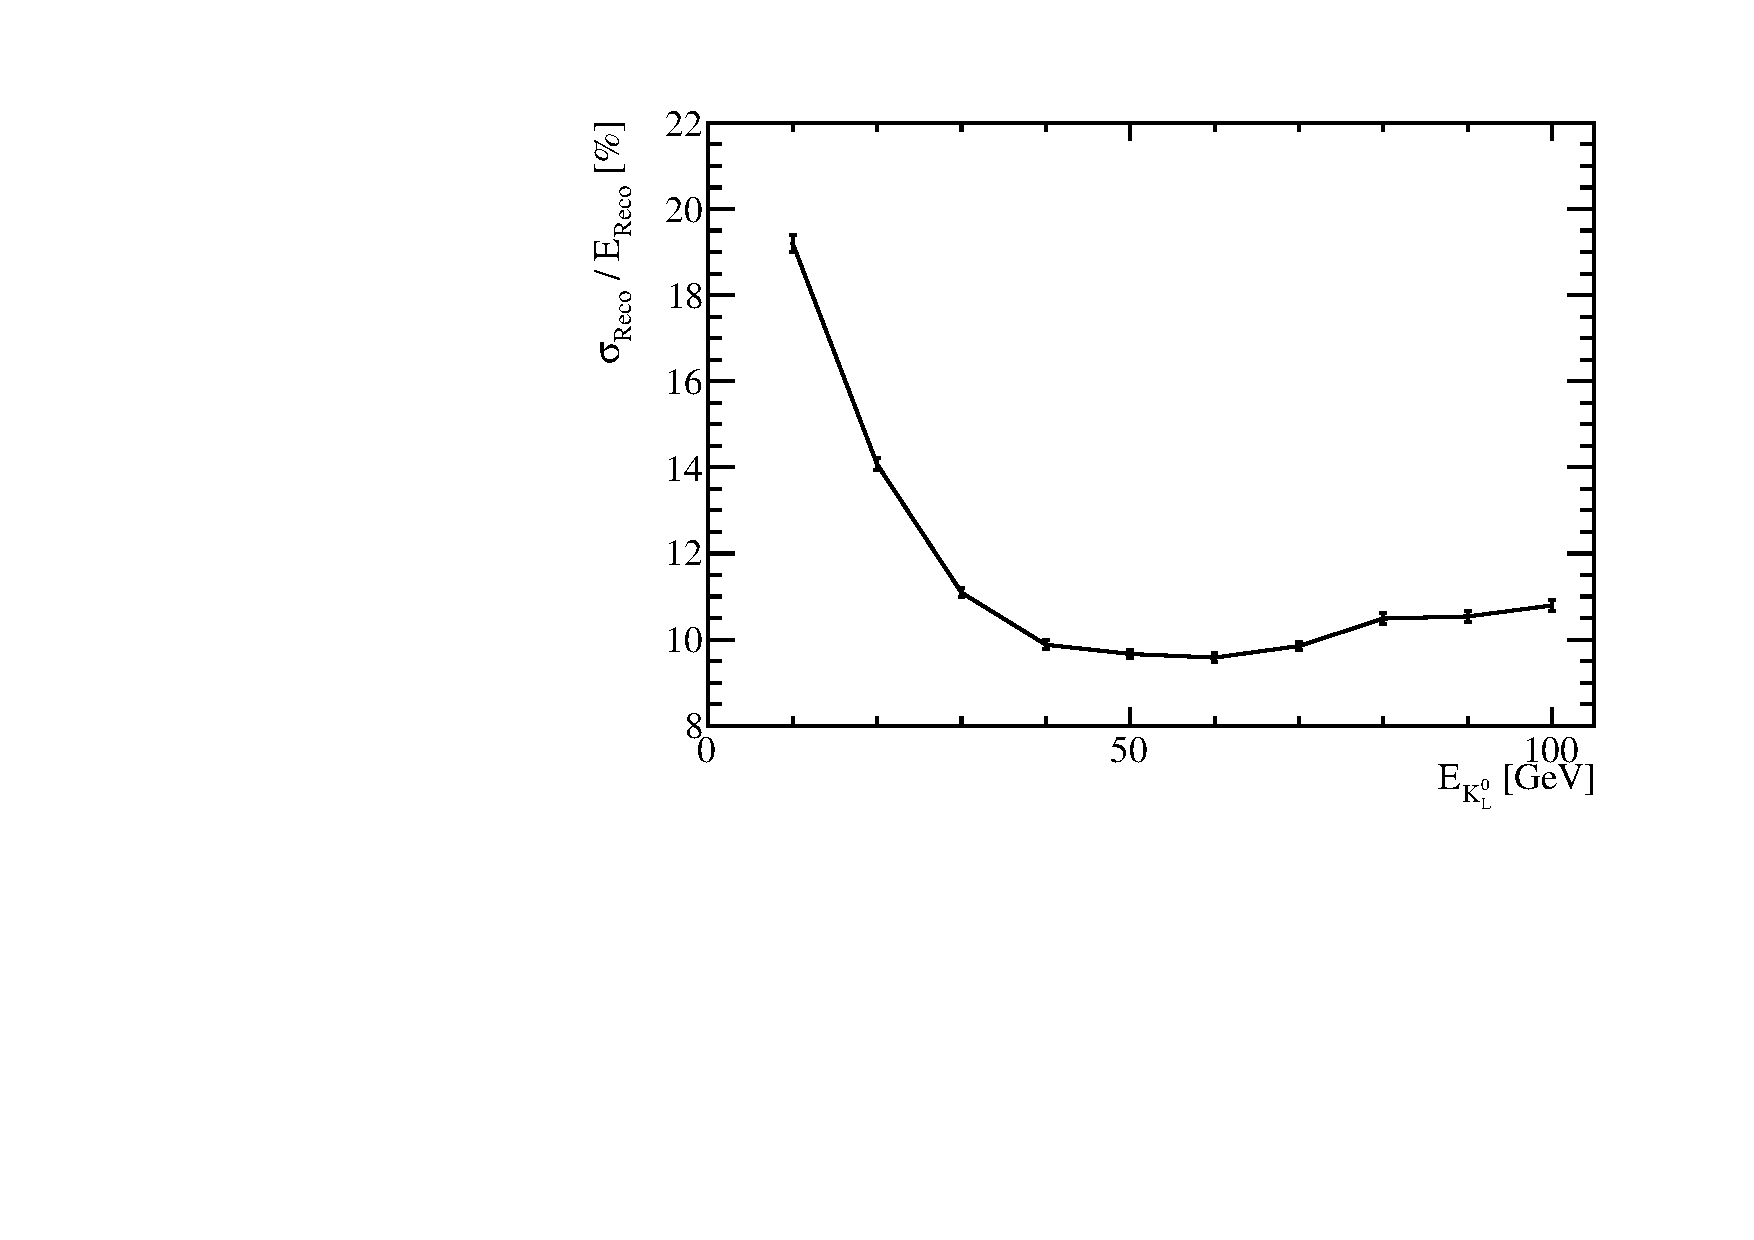
\includegraphics[width=0.5\textwidth]{OptimisationStudies/Plots/EnergyResolution/ER_vs_EKaon0L_SiECal.pdf}}
\subfloat[]{\label{fig:jernominalres}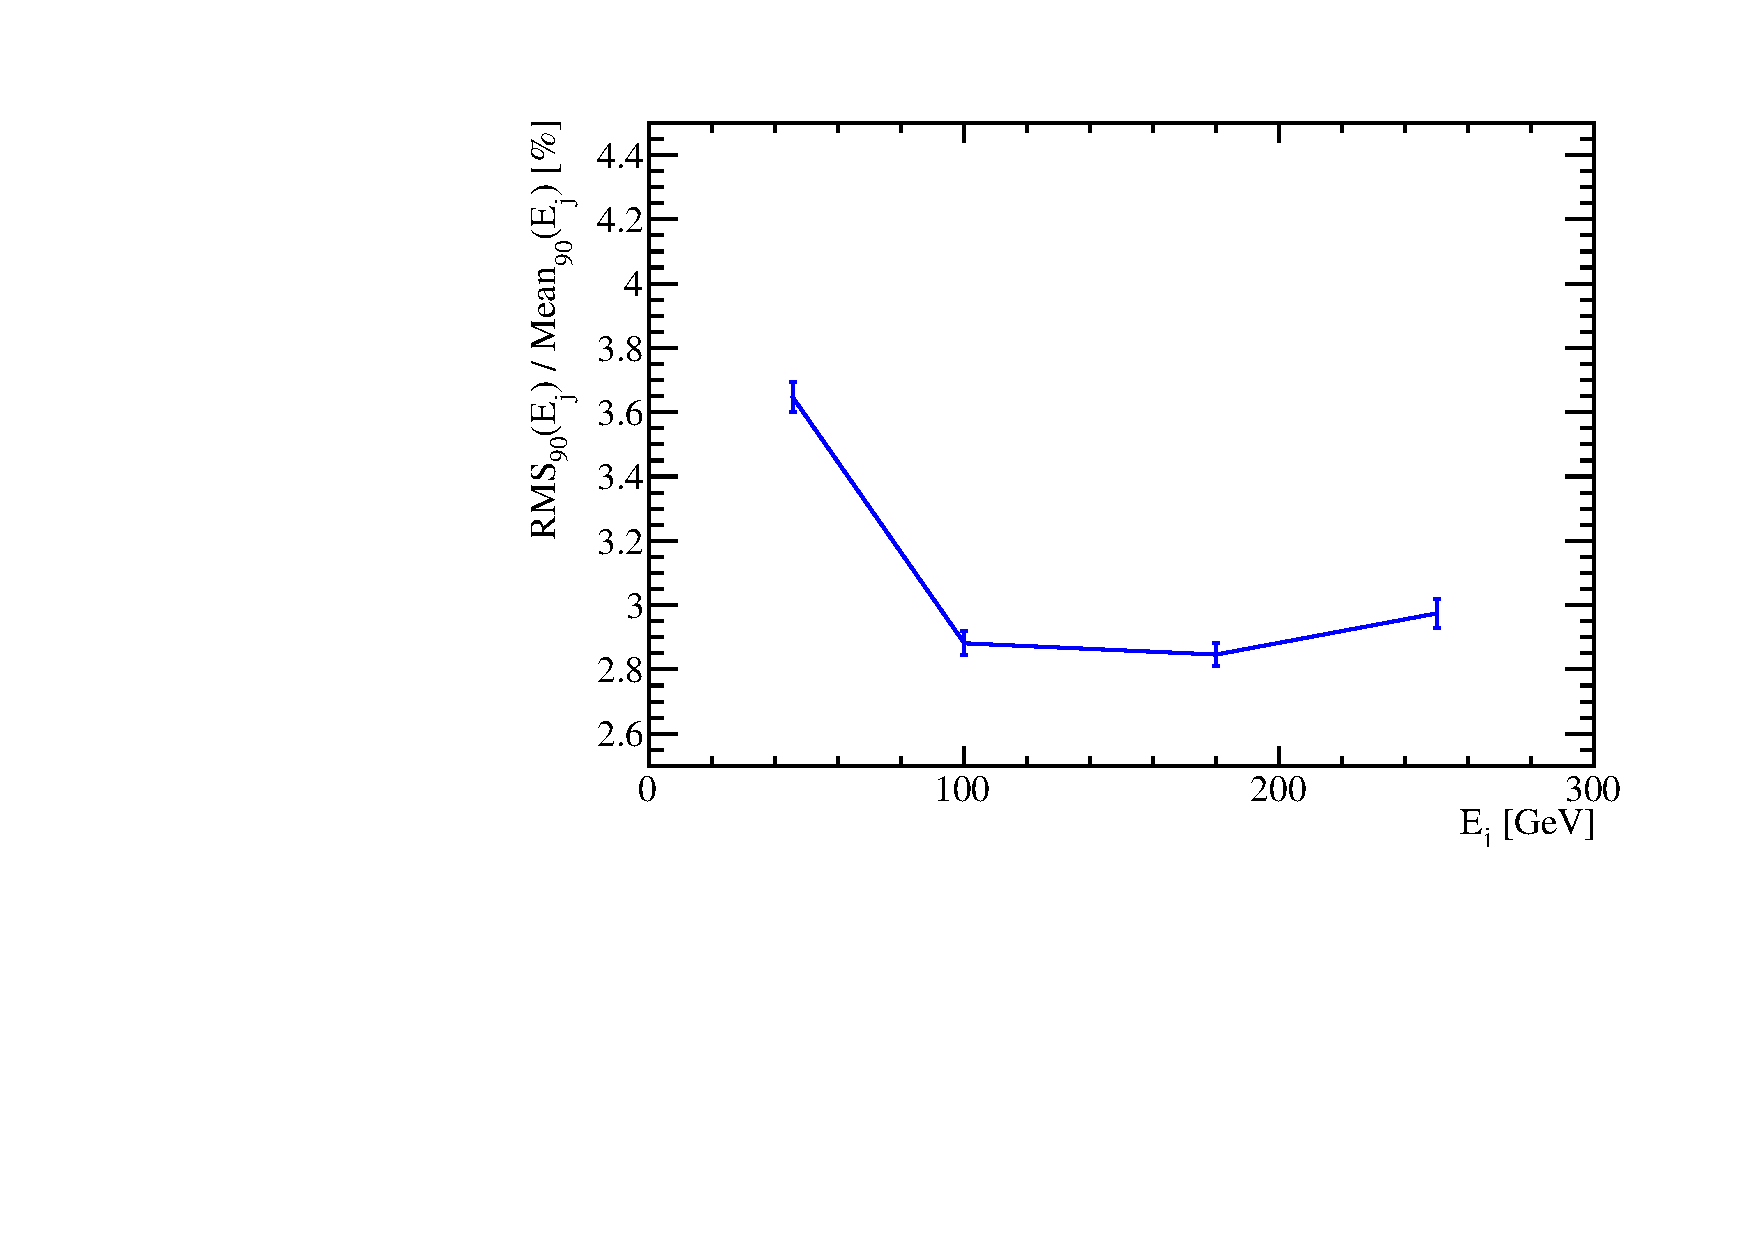
\includegraphics[width=0.5\textwidth]{OptimisationStudies/Plots/JetEnergyResolutions/JER_vs_JetEnergy_NominalDetectorPerformance.pdf}}
\caption[\protect\subref{fig:ecalsinominalres} The energy resolution as a function of $\gamma$ energy using the nominal ILD model for the silicon ECal option.  \protect\subref{fig:ecalscnominalres} The energy resolution as a function of $\gamma$ energy using the nominal ILD model for the scintillator ECal option.  \protect\subref{fig:hcalnominalres} The energy resolution as a function of $K^{0}_{L}$ energy using the nominal ILD model with the silicon ECal option.  \protect\subref{fig:jernominalres} The jet energy resolution ($\text{RMS}_{90}$) as a function of jet energy using the nominal ILD model with the silicon ECal option.  The intrinsic energy resolution and confusion contributions these the jet energy resolutions are also presented.  The black dotted vertical line on the single particle energy resolutions shows the highest energy particles used in the test beam measurements.]{\protect\subref{fig:ecalsinominalres} The energy resolution as a function of $\gamma$ energy using the nominal ILD model for the silicon ECal option.  \protect\subref{fig:ecalscnominalres} The energy resolution as a function of $\gamma$ energy using the nominal ILD model for the scintillator ECal option.  \protect\subref{fig:hcalnominalres} The energy resolution as a function of $K^{0}_{L}$ energy using the nominal ILD model with the silicon ECal option.  \protect\subref{fig:jernominalres} The jet energy resolution ($\text{RMS}_{90}$) as a function of jet energy using the nominal ILD model with the silicon ECal option.  The intrinsic energy resolution and confusion contributions these the jet energy resolutions are also presented.  The black dotted vertical line on the single particle energy resolutions shows the highest energy particles used in the test beam measurements.}
\label{fig:nominalres}
\end{figure}

%========================================================================================
%========================================================================================

\section{Electromagnetic Calorimeter Optimisation}
\label{sec:ecal}
The ECal primarily measures the energy deposits of electromagnetic showers.  The ECal in the nominal ILD detector model, summarised in table \ref{table:defaultildecal}, is a silicon-tungsten sampling calorimeter.  It contains 24 radiation lengths ($\text{X}_{0}$), which is sufficient to contain all but the highest energy electromagnetic showers, and has 29 readout layers.  The absorber thickness of the last nine layers is twice that of the first 20 layers to reduces the number of readout channels and cost of the overall calorimeter while retaining a high sampling rate.  This high sampling rate is crucial for the pattern recognition aspect of particle flow calorimetry, especially in the region where particle showers start developing, as shown in section \ref{sec:ecalcells}.  

\begin{table}[h!]
\centering
\begin{tabular}{ l l}
\hline
Parameter & Default Value \\
\hline
Cell Size & $5 \times 5 \text{mm}^{2}$ square cells \\
Number of Layers & 29 readout layers \\
Active Material Choice & Silicon or Scintillator  \\
Active Material Thickness & 0.5 mm (Silicon) or 2 mm (Scintillator)  \\
Absorber Material Choice & Tungsten \\
Absorber Material Thickness & 20 layers of 2.1 mm followed by 9 layers of 4.2 mm \\
\hline
\end{tabular}
\caption[The configuration of the ECal in the nominal ILD detector model.  The parameters are given for the nominal silicon model as well as the alternative scintillator option.]{The configuration of the ECal in the nominal ILD detector model.  The parameters are given for the nominal silicon model as well as the alternative scintillator option.}
\label{table:defaultildecal}
\end{table}

The calorimeter performance was simulated for a number of detector models where the following detector parameters were varied:
\begin{itemize}
\item Cell size:  This is a vital aspect of the detector in the particle flow paradigm as smaller cell sizes give greater potential for being able to separate energy deposits from charged and neutral particles.  This should have little to no effect on the intrinsic energy resolution of the detector.  
\item Number of layers or sampling frequency:  When varying the number of layers the layer thicknesses are altered to keep the total number of radiation lengths within the ECal constant.  By increasing the number of layers in the calorimeter a particle shower is sampled more thoroughly leading to a reduction in the stochastic contribution to the energy resolution.  Therefore, the number of layers will govern the intrinsic energy resolution of the calorimeter.
\item Active material choice:  The options under consideration for the active material choice are silicon or scintillator.  As well as providing different intrinsic energy resolutions the readout mechanics of these two options are significantly different.  There is no clear prior knowledge as to which should provide better performance. 
\end{itemize}

%========================================================================================

\subsection{ECal Cell Size}
\label{sec:ecalcells}
A number of different detector models were considered where the cell size in the ECal was varied about the nominal value of $5 \times 5 \text{mm}^{2}$ square cells.  The granularities considered were $3 \times 3 \text{mm}^{2}$, $5 \times 5 \text{mm}^{2}$, $7 \times 7 \text{mm}^{2}$, $10 \times 10 \text{mm}^{2}$, $15 \times 15 \text{mm}^{2}$ and $20 \times 20 \text{mm}^{2}$ square cells for both the silicon and scintillator active material options.  

The energy resolution, using 100 GeV $\gamma$ events, as a function of the ECal cell size is shown in figure \ref{fig:ecalsicellsize} for the silicon option and figure \ref{fig:ecalsccellsize} for the scintillator option.  As at these energies the $\gamma$ will be largely contained within the ECal, these results relate solely to the energy resolution of the ECal within the full ILD simulation.  For both the silicon and scintillator ECal options the energy resolution does not depend strongly on the ECal cell size.  This is to be expected as the sampling frequency, which is the main factor in determining the energy resolution of a calorimeter, does not change when modifying the cell size.  There are minor fluctuations in the energy resolution when varying the cell size, but these are mostly likely due to fluctuations in the energy response from calibration procedure that was applied to each detector models.  For the scintillator ECal option there is a significant degradation in the energy resolution for the $3 \times 3 \text{mm}^{2}$ cell size model.  The most likely cause of this is a "dead" region in the active material, which represents the readout multi pixel photon counter (MPPC) \ref{arXiv:1006.3396}.  The MPPC occupies a fixed area of the cell irrespective of cell size and so the dead region of the cell fractionally increases as cell size is reduced.  The larger this dead region, the worse the sampling of the electromagnetic showers in the ECal and the worse the resolution.  While this effect will be present in all scintillator ECal options, it will only be significant for the small cell sizes when the dead region is fractionally the largest.  This explains why degradation is seen only for the smallest cell size considered in the scintillator ECal option.     

\begin{figure}[h!]\centering
\subfloat[]{\label{fig:ecalsicellsize100gamma}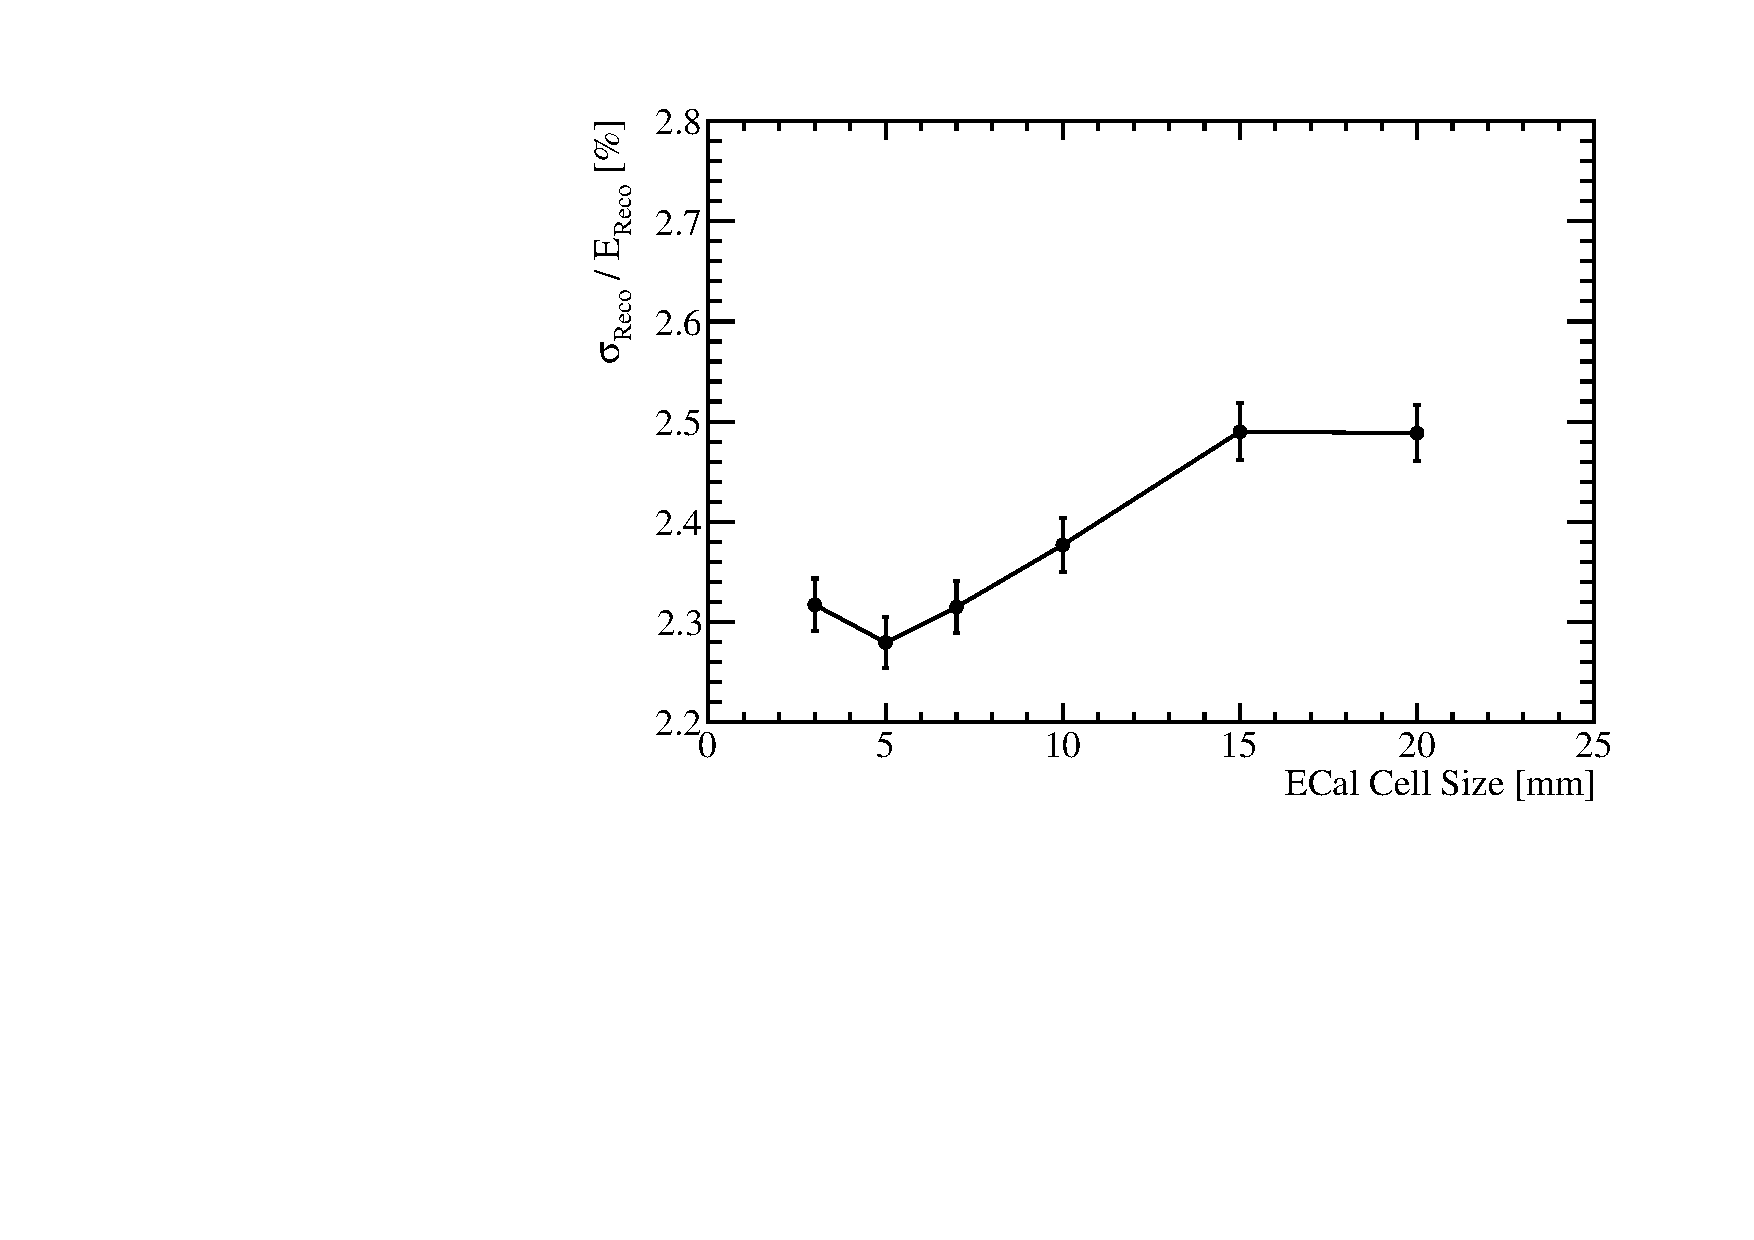
\includegraphics[width=0.5\textwidth]{OptimisationStudies/Plots/EnergyResolution/ER_vs_SiECalCellSize_100GeVPhoton.pdf}}
\subfloat[]{\label{fig:ecalsccellsize100gamma}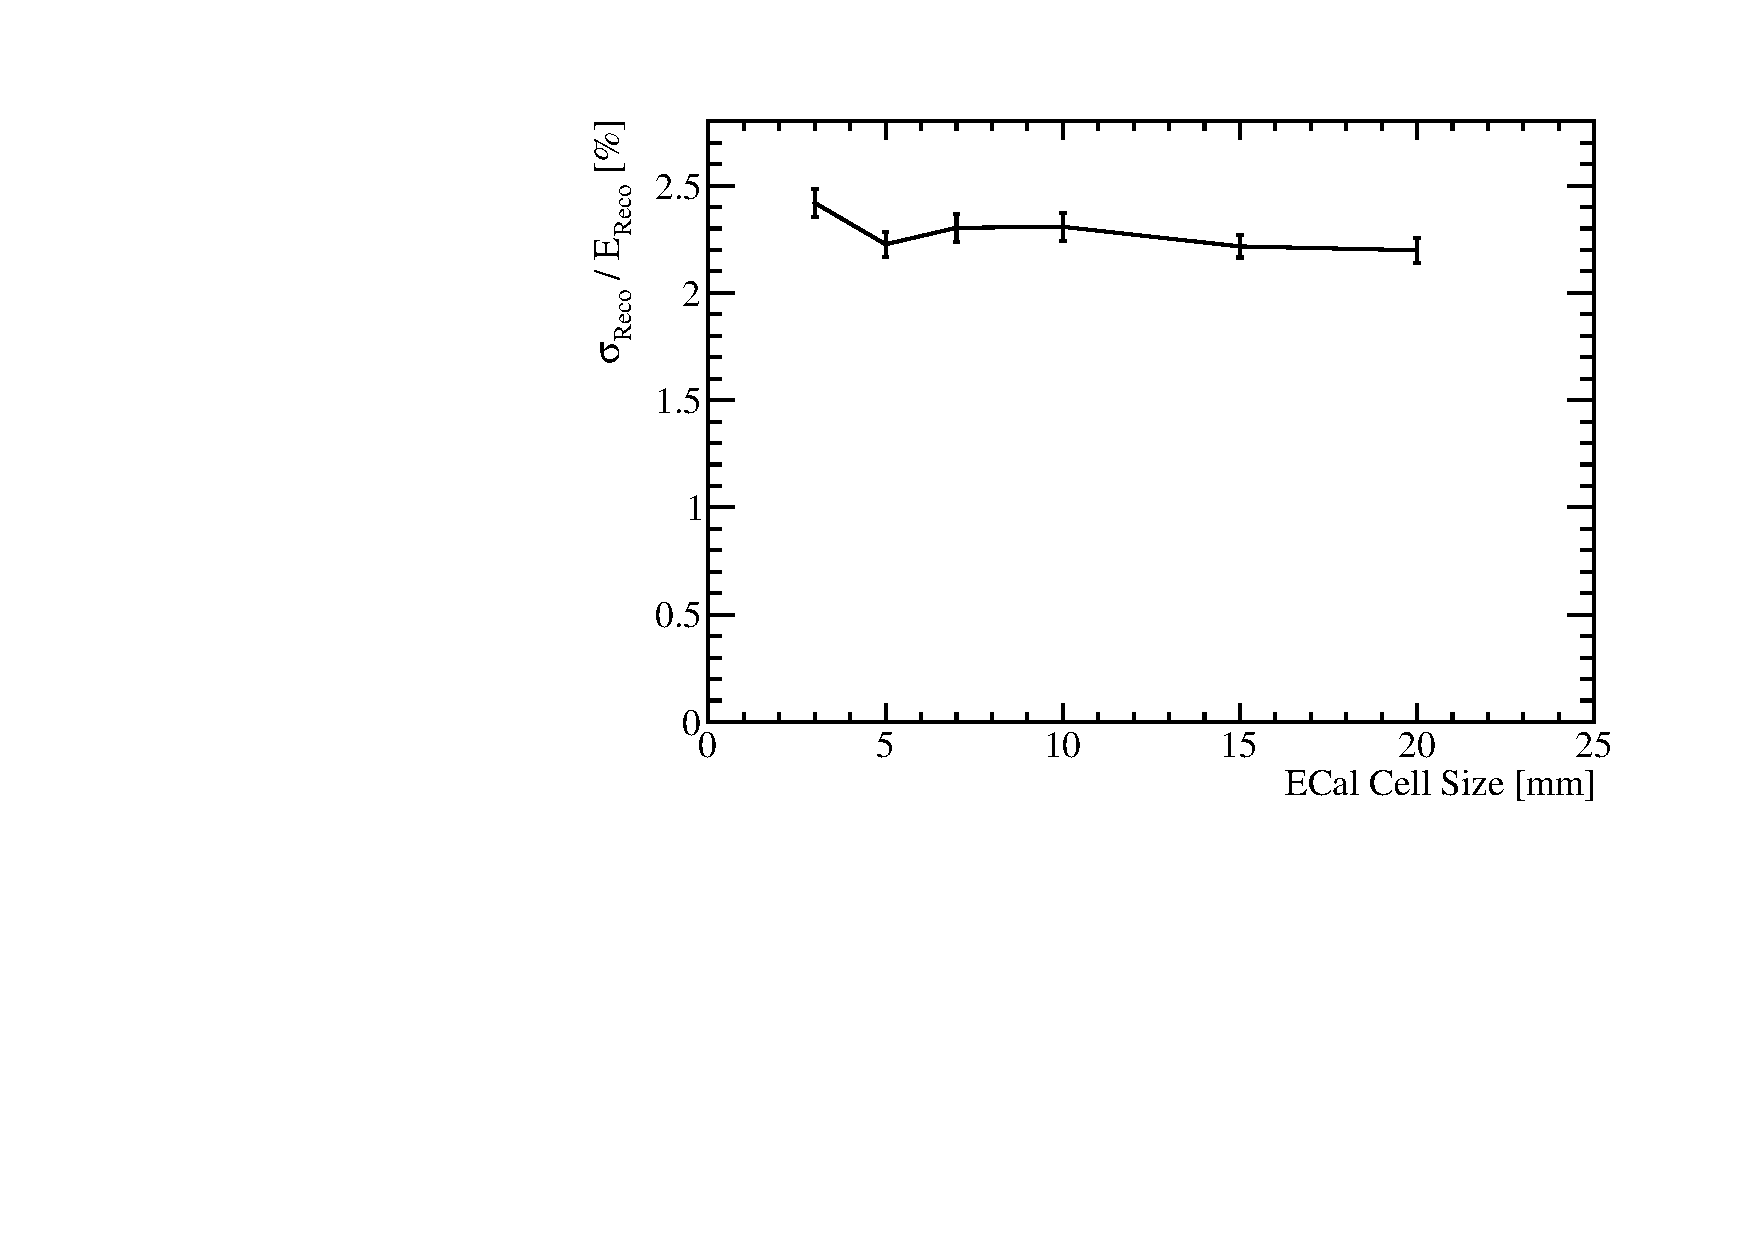
\includegraphics[width=0.5\textwidth]{OptimisationStudies/Plots/EnergyResolution/ER_vs_ScECalCellSize_100GeVPhoton.pdf}}
\caption[The energy resolution as a function of ECal cell size for 100 GeV $\gamma$s using the nominal ILD detector model with \protect\subref{fig:ecalsicellsize100gamma} the silicon and \protect\subref{fig:ecalsccellsize100gamma} the scintillator ECal option.]{The energy resolution as a function of ECal cell size for 100 GeV $\gamma$s using the nominal ILD detector model with \protect\subref{fig:ecalsicellsize100gamma} the silicon and \protect\subref{fig:ecalsccellsize100gamma} the scintillator ECal option.}
\label{fig:ecalcellsizegamma}
\end{figure}

The separation of nearby particle showers within the calorimeter is limited by the cell size.  Smaller cell sizes make it easier to separate nearby particle showers, which causes a reduction in the affect of confusion.  Therefore, although the intrinsic energy resolution of a calorimeter is not dependent on the cell size, it is expected that the jet energy resolution be sensitive to the ECal cell size.  The jet energy resolution as a function of ECal cell size is shown in figure \ref{fig:ecalsicellsize} for the silicon option and figure \ref{fig:ecalsccellsize} for the scintillator option.  As expected there is a very strong dependancy on the ECal cell size, with smaller cell sizes leading to lower values of the jet energy resolution.  The origin of this trend is best illustrated by considering the intrinsic energy resolution and confusion contributions to the jet energy resolution.  These contributions are shown as a function of ECal cell size for 45 and 250 GeV jets, for both the silicon and scintillator ECal options, in figure \ref{fig:ecalcellsizebreak}.  It is clear from these contributions that the intrinsic energy resolution of the detector does not change when varying the cell size, which agrees with both prior expectations of calorimeter behaviour and the single particle energy resolution study.  The minor fluctuations seen in the energy resolution for the single particle study are washed out when considering the intrinsic energy resolution for jets, as only $~30\%$ of jet energy is carried in the form of $\gamma$s.  Furthermore, the jet energy resolution trend as a function of the ECal cell size is being driven purely by changes to the confusion contribution and, in particular, the confusion caused by the reconstruction of $\gamma$s.  This is exactly what is to expected given the ECal primarily measures $\gamma$s and shows that the performance of the ECal when varying the cell size is well understood.

\begin{figure}[h!]
\centering
\subfloat[]{\label{fig:ecalsicellsize}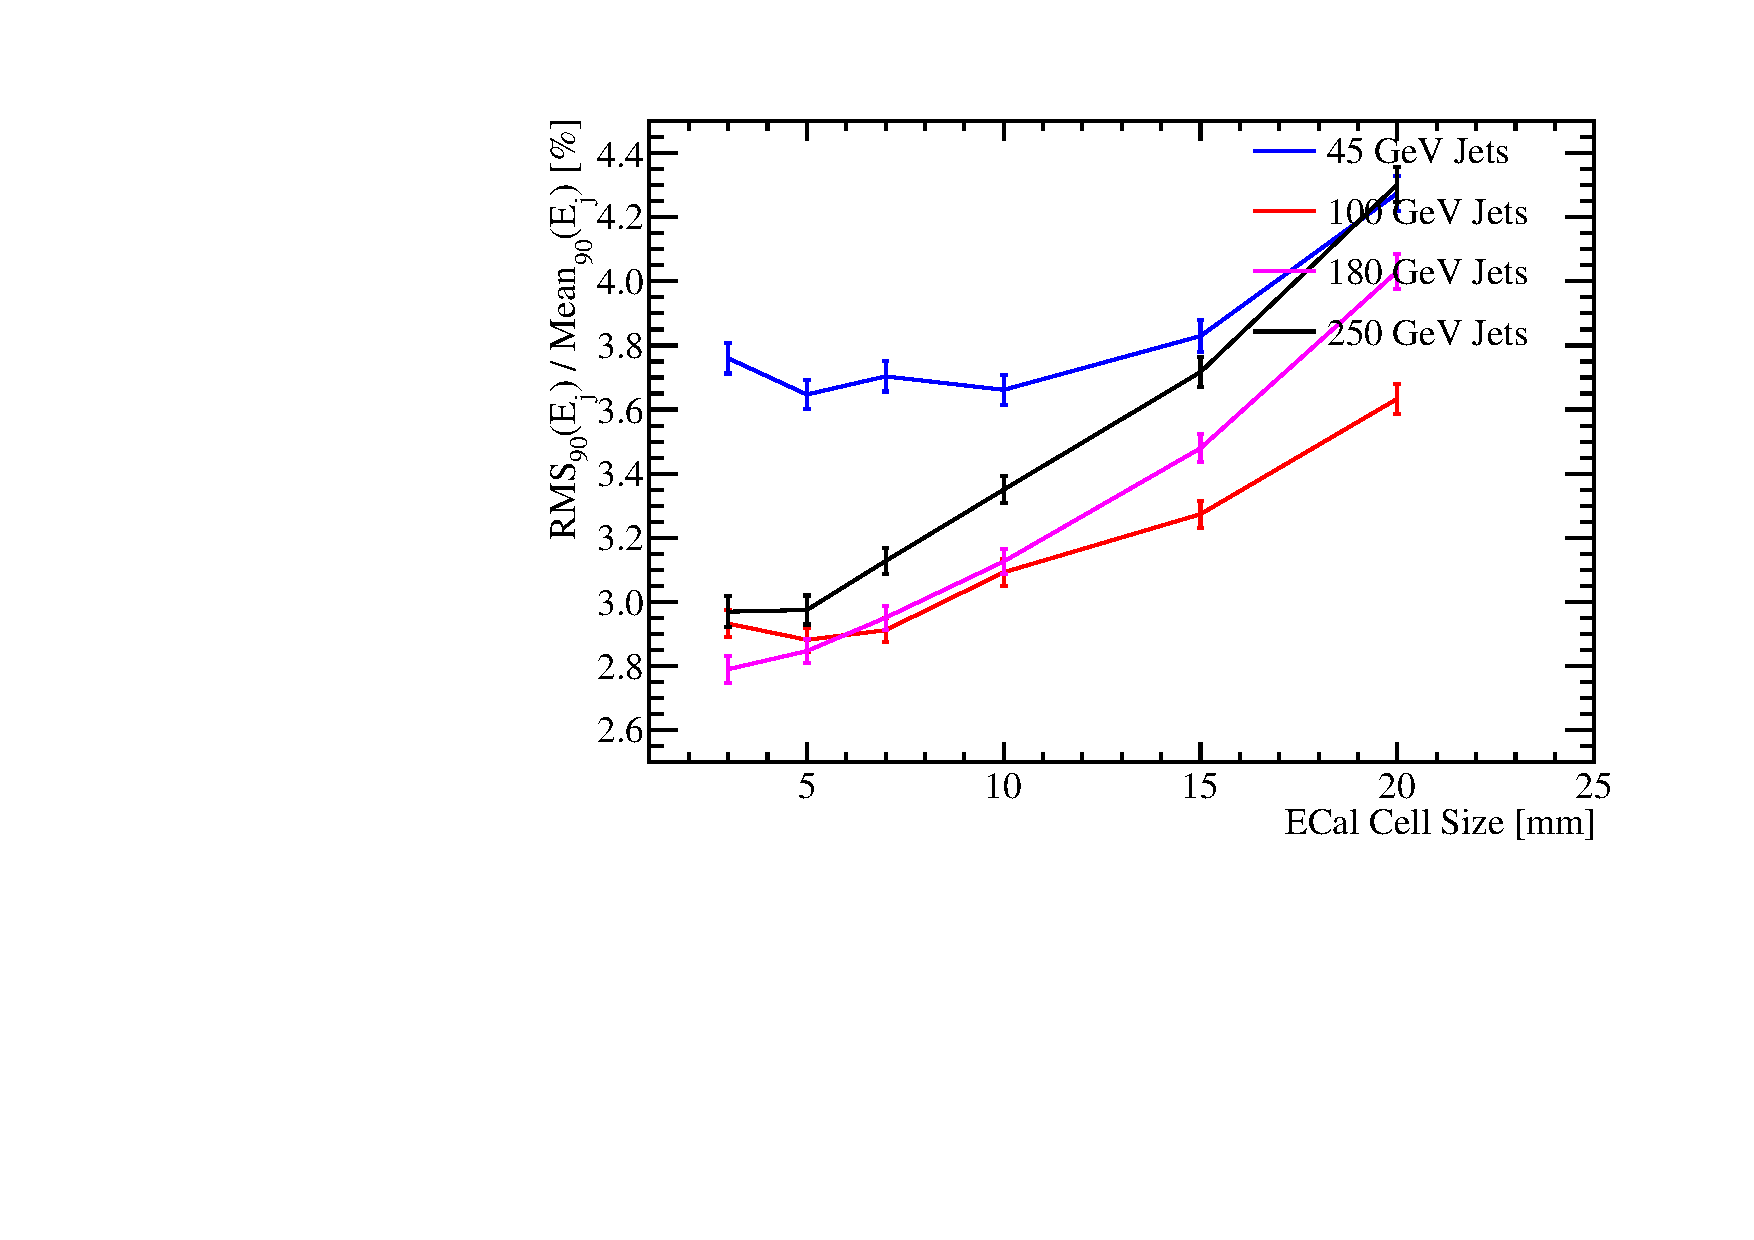
\includegraphics[width=0.5\textwidth]{OptimisationStudies/Plots/JetEnergyResolutions/JER_vs_SiliconECalCellSize.pdf}}
\subfloat[]{\label{fig:ecalsccellsize}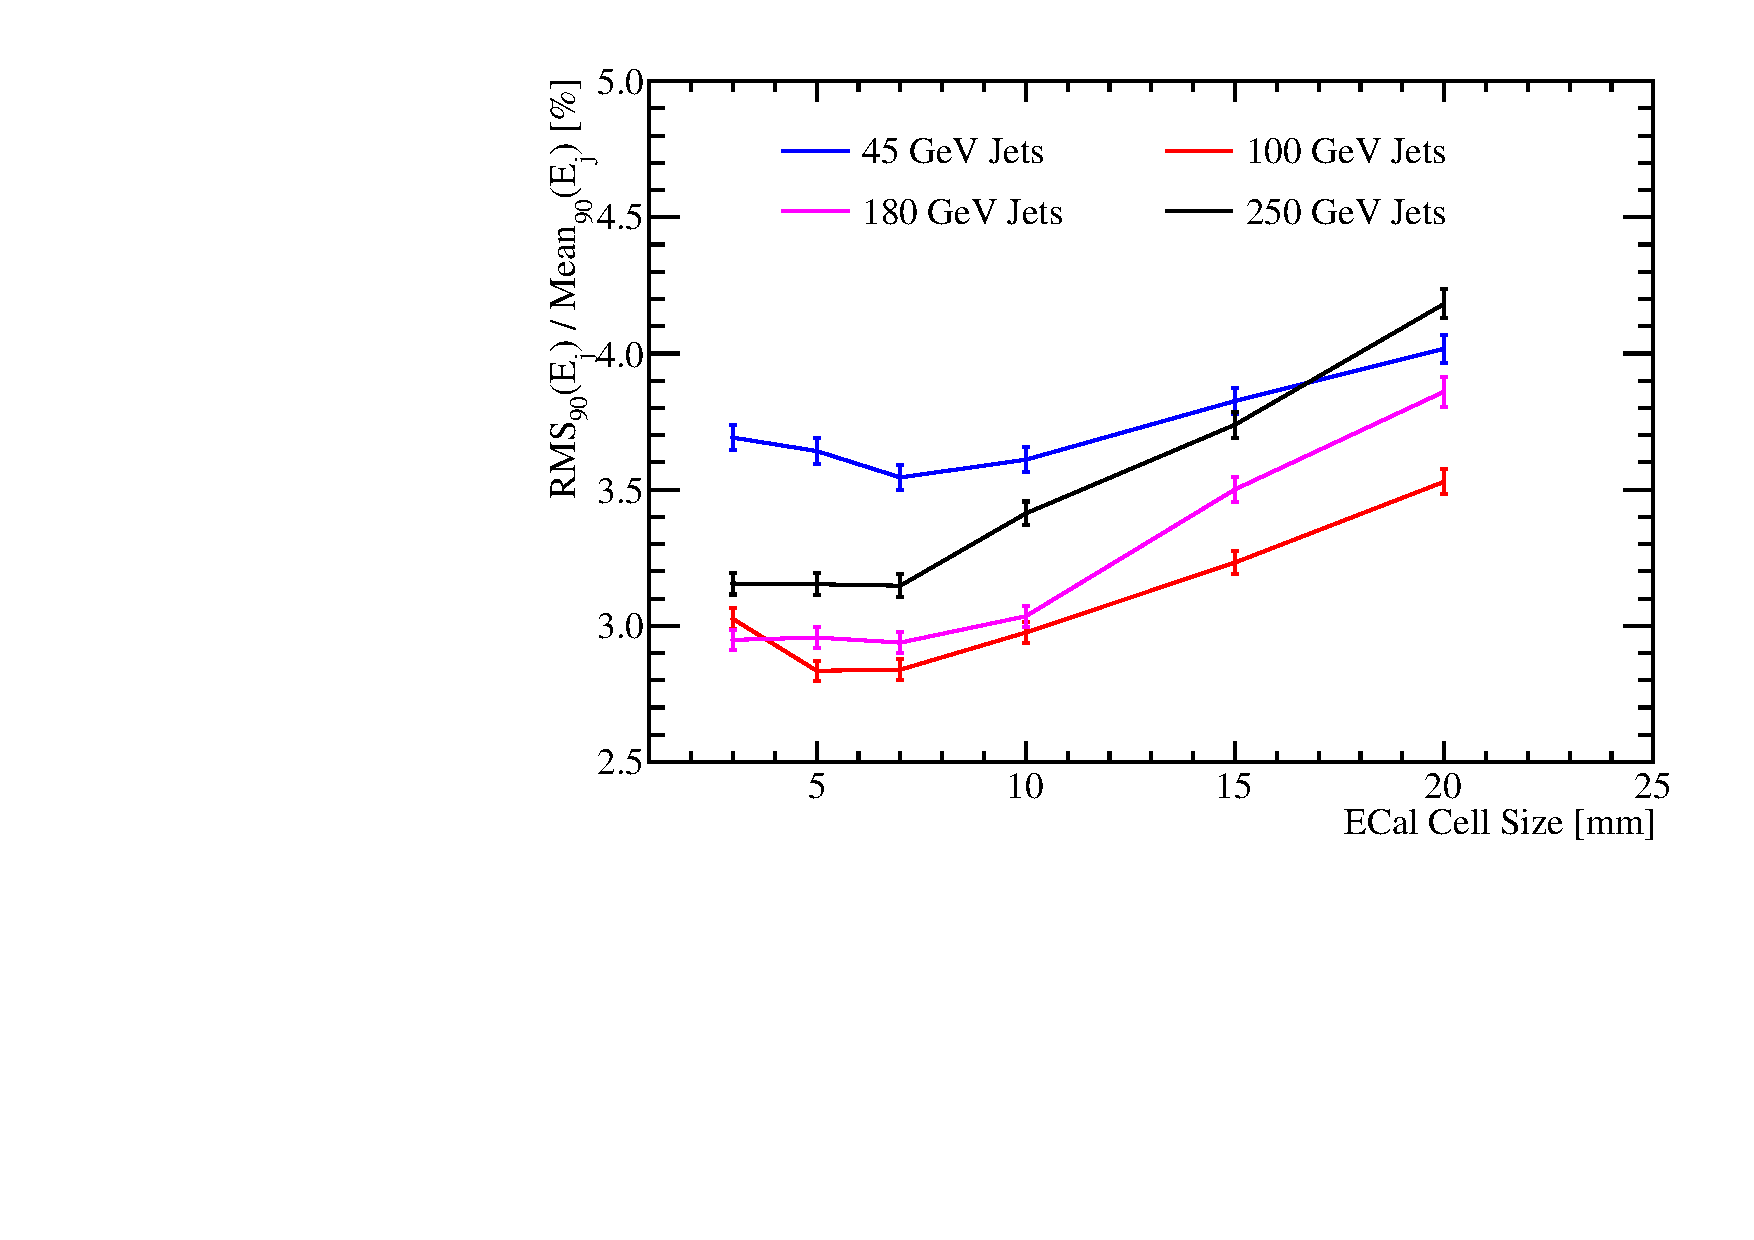
\includegraphics[width=0.5\textwidth]{OptimisationStudies/Plots/JetEnergyResolutions/JER_vs_ScintillatorECalCellSize.pdf}} \hfill
\caption[The jet energy resolution as a function of ECal cell size for various jet energies using the nominal ILD detector model with \protect\subref{fig:ecalsicellsize} the silicon and \protect\subref{fig:ecalsccellsize} the scintillator ECal option.]{The jet energy resolution as a function of ECal cell size for various jet energies using the nominal ILD detector model with \protect\subref{fig:ecalsicellsize} the silicon and \protect\subref{fig:ecalsccellsize} the scintillator ECal option.}
\label{fig:ecalcellsize}
\end{figure}

\begin{figure}[h!]
\centering
\subfloat[]{\label{fig:ecalsicellsize45break}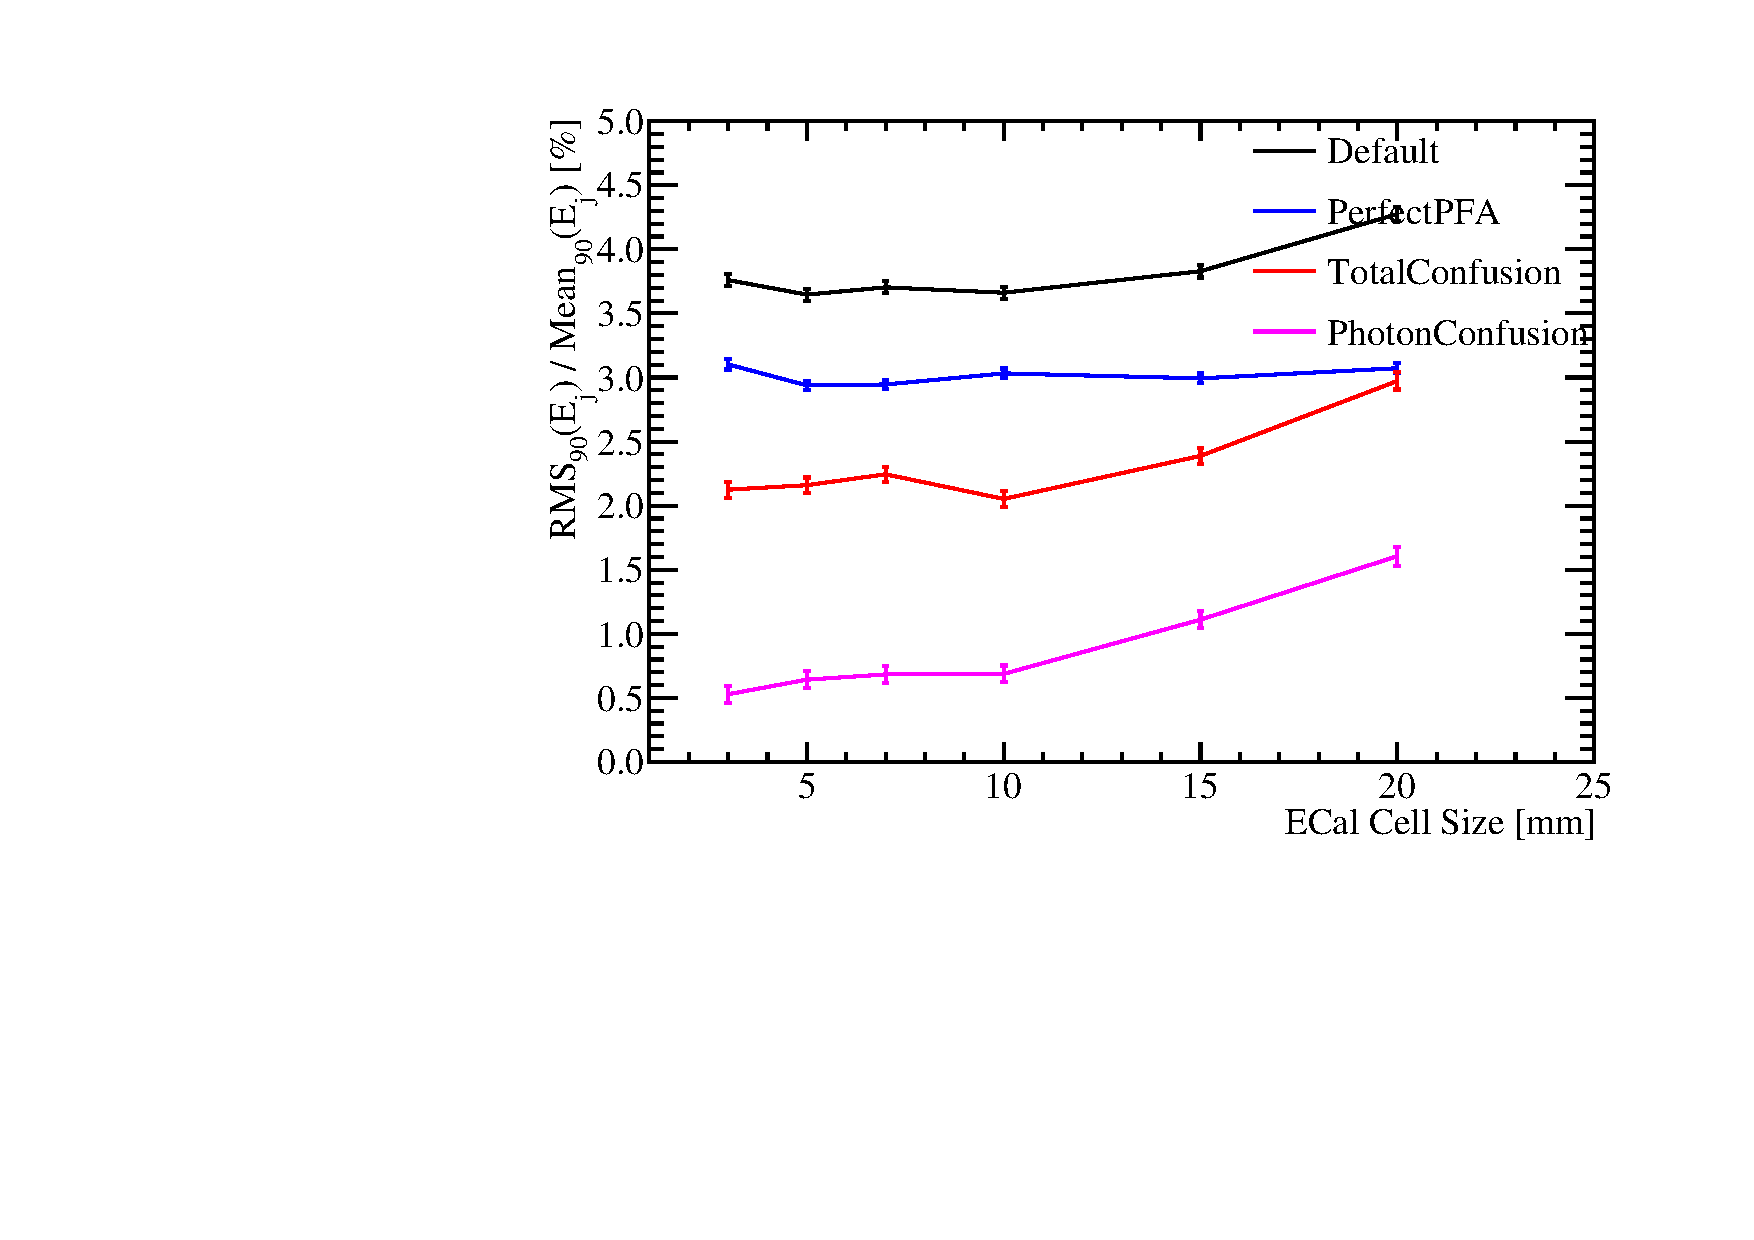
\includegraphics[width=0.5\textwidth]{OptimisationStudies/Plots/JetEnergyResolutions/JER_vs_SiliconECalCellSize_91GeV_DiJet_Breakdown.pdf}}
\subfloat[]{\label{fig:ecalsccellsize45break}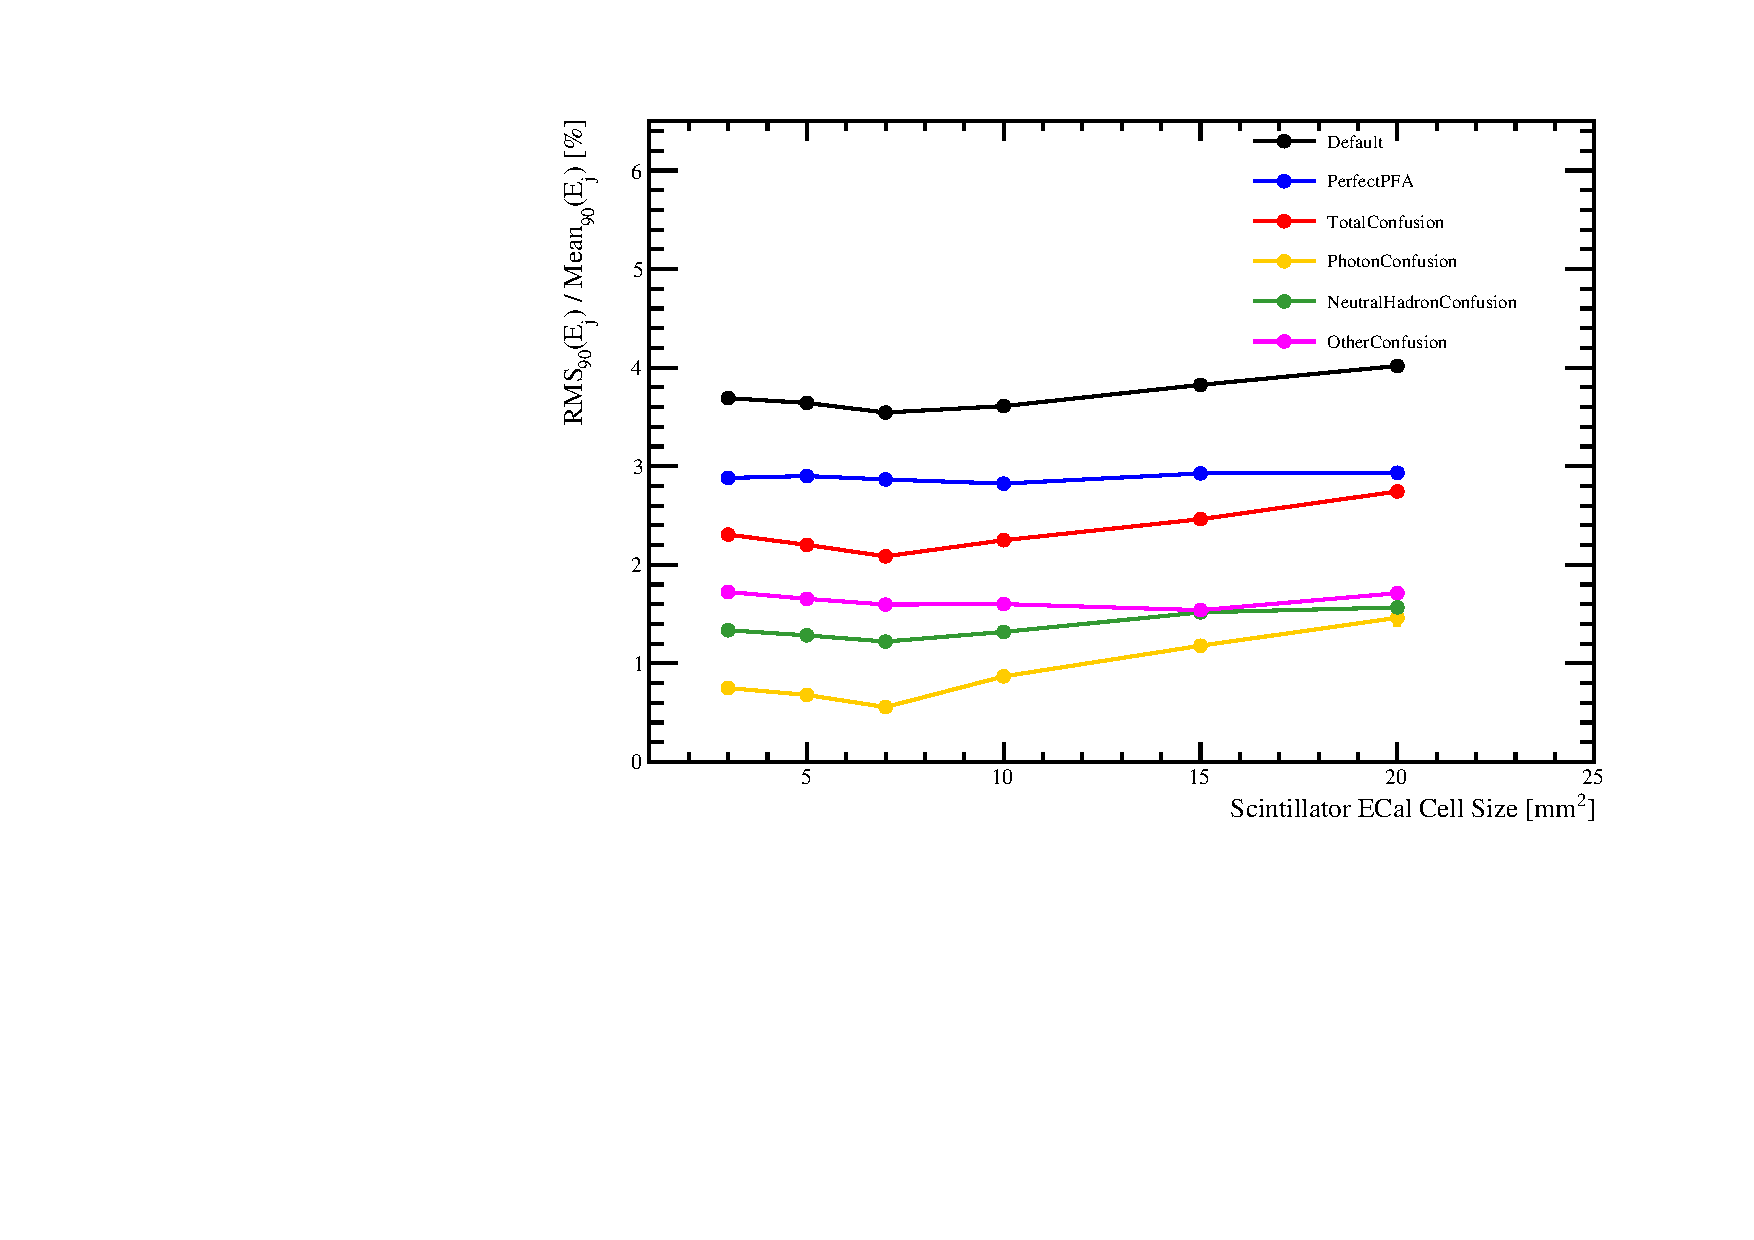
\includegraphics[width=0.5\textwidth]{OptimisationStudies/Plots/JetEnergyResolutions/JER_vs_ScintillatorECalCellSize_91GeV_DiJet_Breakdown.pdf}} \hfill
\subfloat[]{\label{fig:ecalsicellsize250break}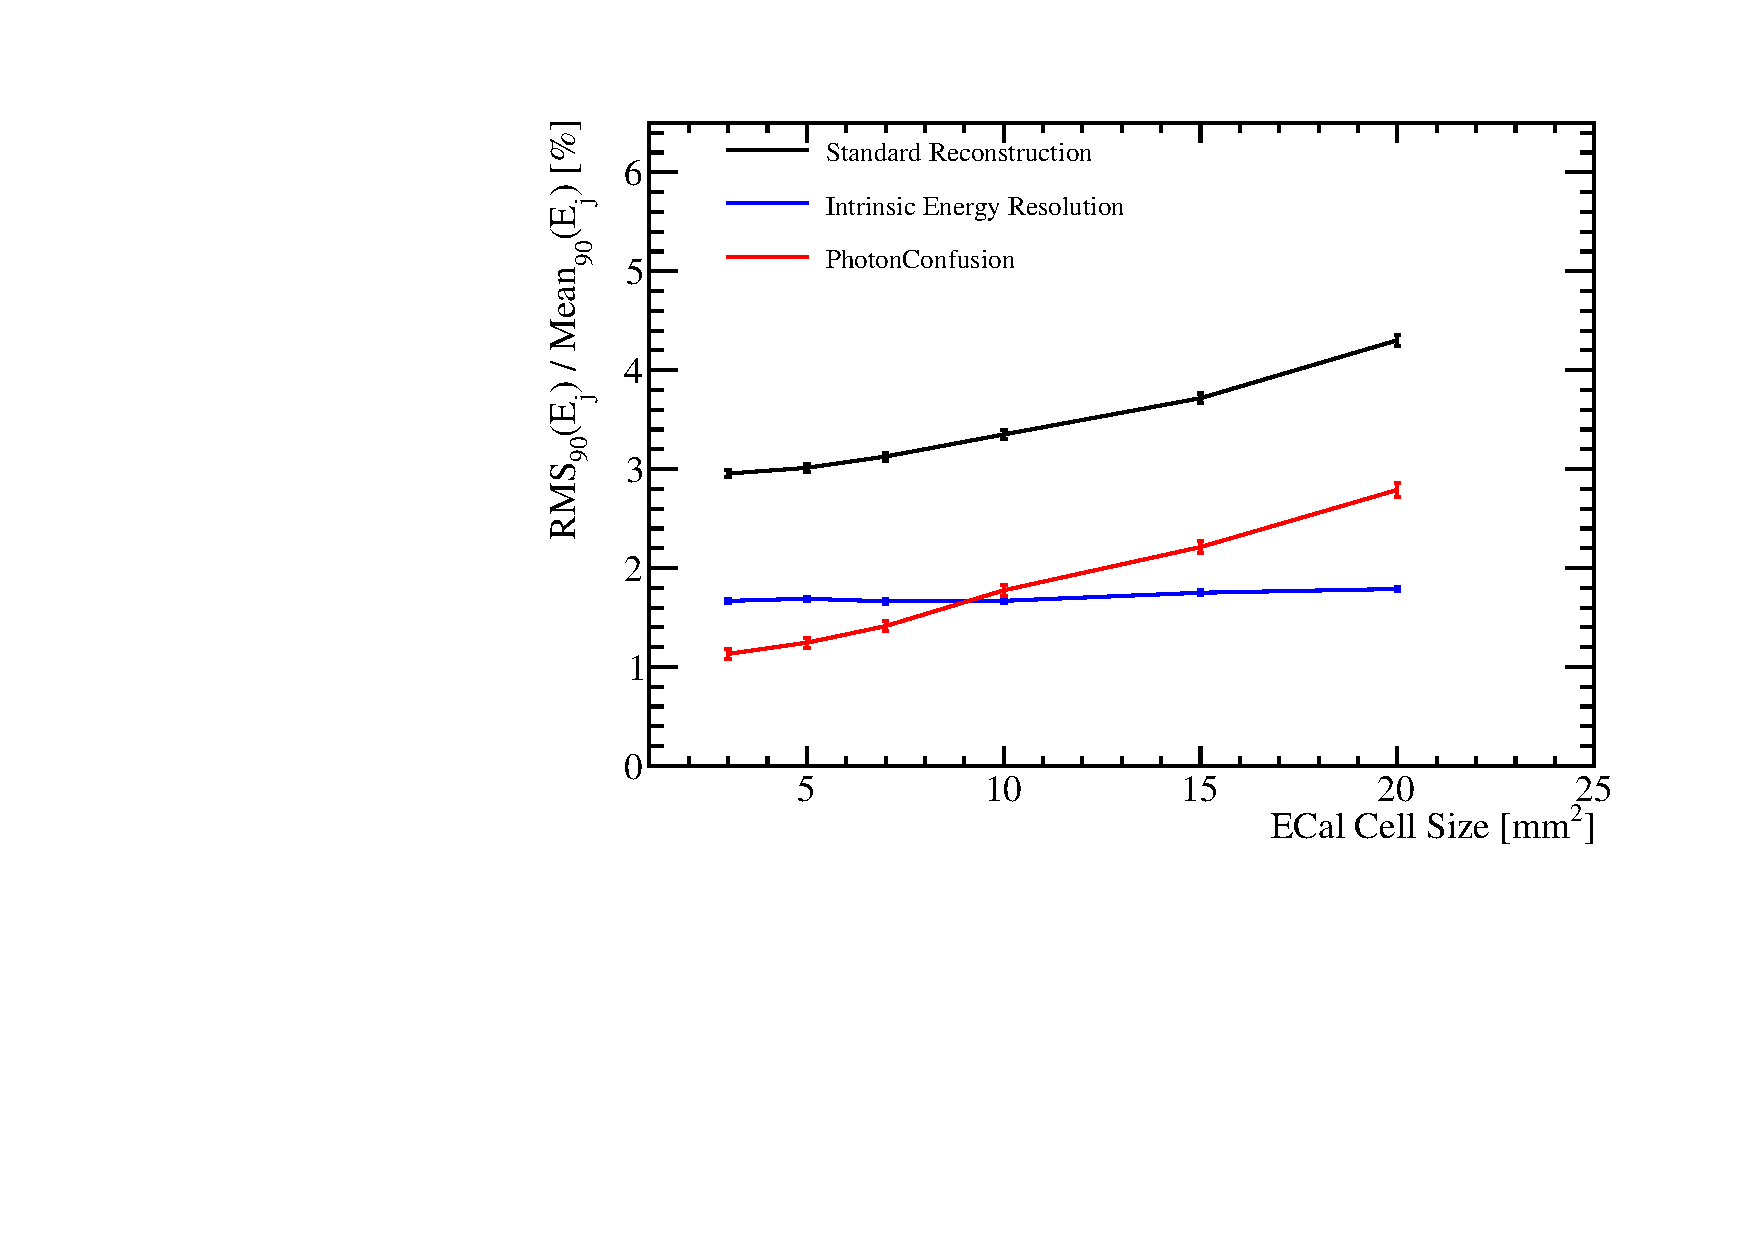
\includegraphics[width=0.5\textwidth]{OptimisationStudies/Plots/JetEnergyResolutions/JER_vs_SiliconECalCellSize_500GeV_DiJet_Breakdown.pdf}}
\subfloat[]{\label{fig:ecalsccellsize250break}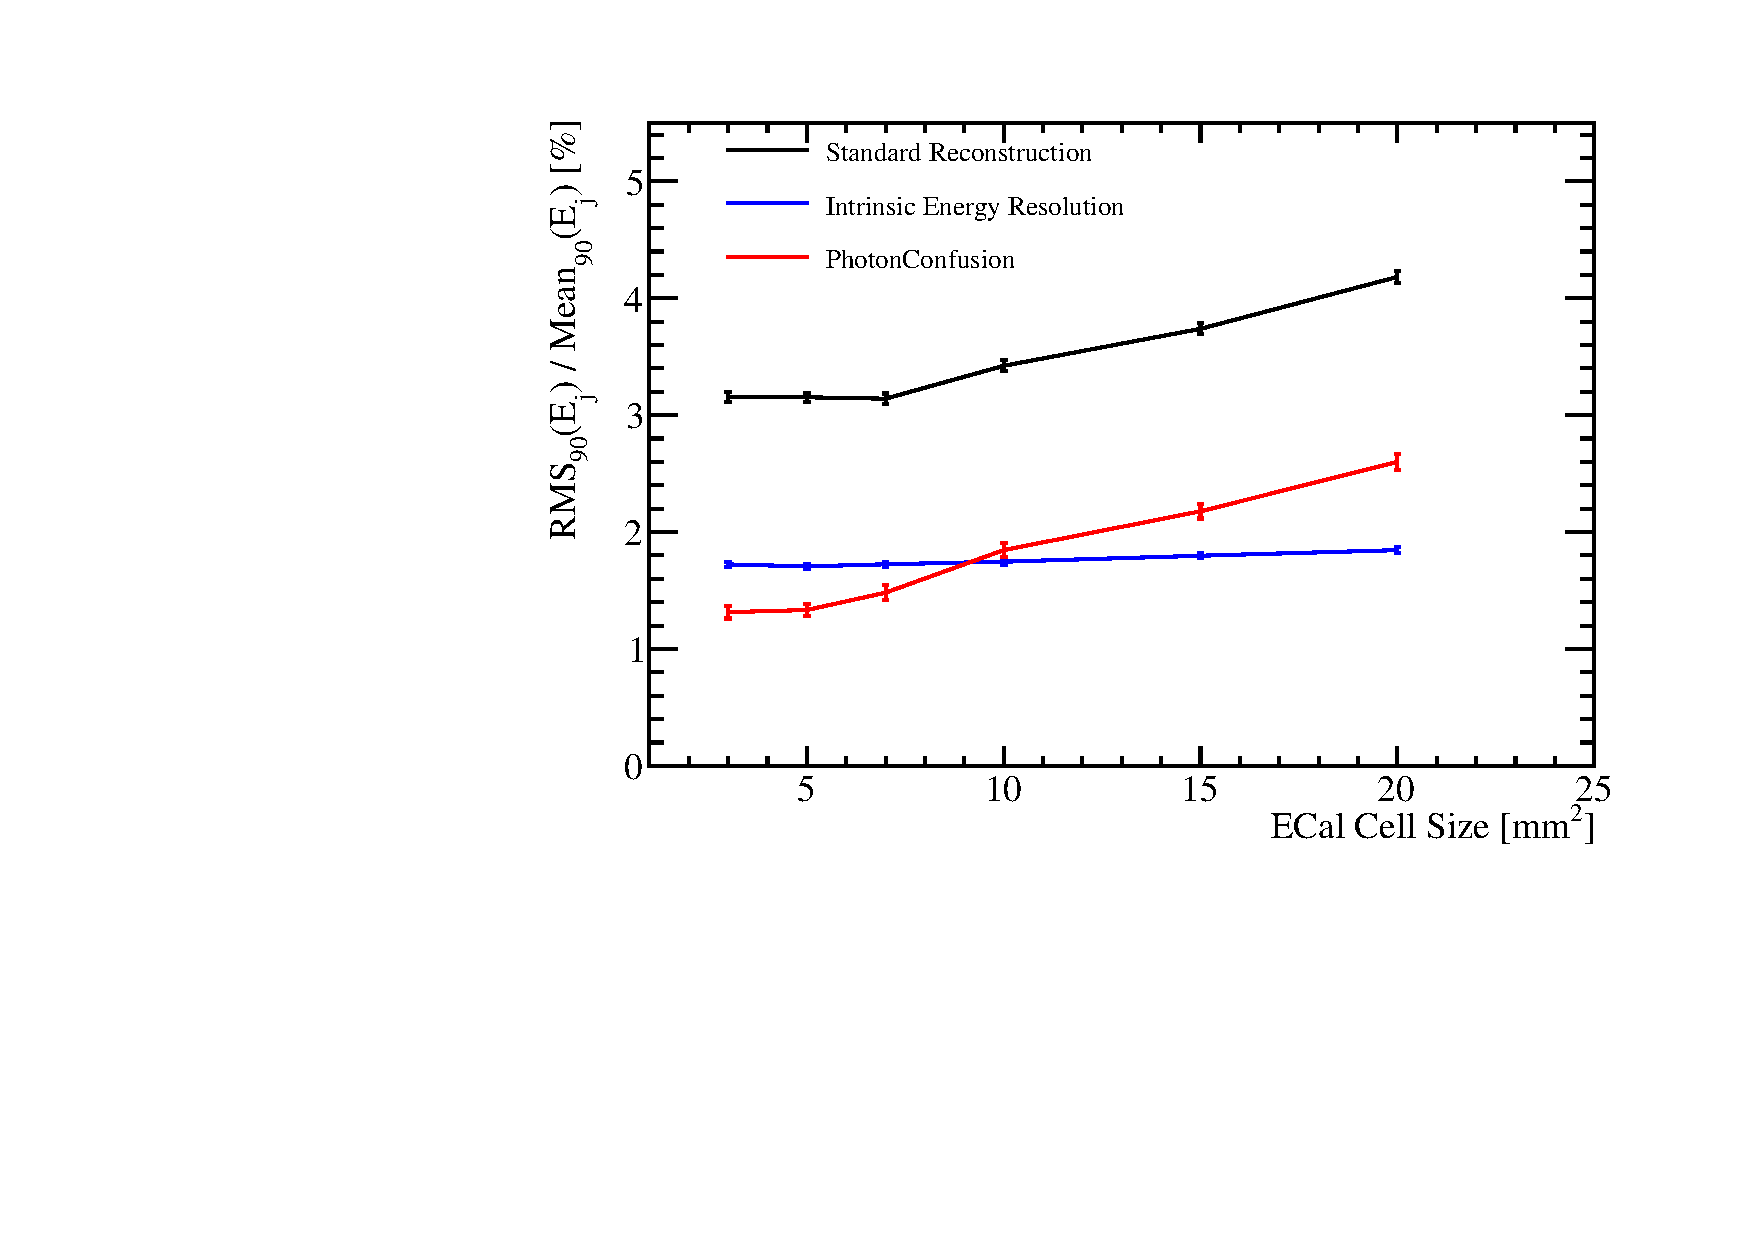
\includegraphics[width=0.5\textwidth]{OptimisationStudies/Plots/JetEnergyResolutions/JER_vs_ScintillatorECalCellSize_500GeV_DiJet_Breakdown.pdf}}
\caption[The contributions to the jet energy resolution as a function of ECal cell size using the nominal ILD detector model for \protect\subref{fig:ecalsicellsize45break} the silicon ECal option and 45 GeV jets, \protect\subref{fig:ecalsccellsize45break} the scintillator ECal option and 45 GeV jets, \protect\subref{fig:ecalsicellsize250break} the silicon ECal option and 250 GeV jets and \protect\subref{fig:ecalsccellsize250break} the scintillator ECal option and 250 GeV jets.  The black curves correspond to the standard reconstruction, the blue curves to the intrinsic energy resolution contribution to the jet energy resolution, the red curves to the confusion contribution to the jet energy resolution and the magenta curves to the confusion contribution to the jet energy resolution related solely to $\gamma$ reconstruction.]{The contributions to the jet energy resolution as a function of ECal cell size using the nominal ILD detector model for \protect\subref{fig:ecalsicellsize45break} the silicon ECal option and 45 GeV jets, \protect\subref{fig:ecalsccellsize45break} the scintillator ECal option and 45 GeV jets, \protect\subref{fig:ecalsicellsize250break} the silicon ECal option and 250 GeV jets and \protect\subref{fig:ecalsccellsize250break} the scintillator ECal option and 250 GeV jets.  The black curves correspond to the standard reconstruction, the blue curves to the intrinsic energy resolution contribution to the jet energy resolution, the red curves to the confusion contribution to the jet energy resolution and the magenta curves to the confusion contribution to the jet energy resolution related solely to $\gamma$ reconstruction}
\label{fig:ecalcellsizebreak}
\end{figure}

It is clear that the ECal cell size is extremely important for the jet energy resolution of the detector, but it has little bearing on the intrinsic energy resolution.  To ensure separation of hadronic decays of W and Z bosons is possible at ILC like energies, an ECal cell size of least $15 \times 15 \text{mm}^{2}$ is crucial, however, as reducing the ECal cell size further continues to improve the jet energy resolution choosing the smallest size possible is desirable.   

%========================================================================================

\subsection{ECal Number of Layers}curves 
\label{sec:ecalnlayers}
The ECal performance was simulated for different numbers of sampling layers, while keeping the total material budget ($\text{X}_{0}$) approximately constant.  This study was performed for both the silicon and scintillator active material options.  In all cases tungsten was used for the ECal absorber material and the active layer thicknesses were not changed from those used in the nominal ECal models found in table \ref{table:defaultildecal}.  The different layouts for the ECals considered here are summarised in table \ref{table:nlayersecaloption}.  

\begin{table}[h!]
\centering
\begin{tabular}{ l l l l l l}
\hline
Total Number & $N_{Layers}$ & Absorber & $N_{Layers}$ & Absorber & Total  \\
of Layers & Region 1 & Thickness & Region 2 & Thickness & Thickness \\
$N_{\text{Layers ECal}}$ & & Region 1 [mm] & &  Region 2 [mm] &  [$\text{X}_{0}$] \\
\hline
30 & 20 & 2.10 & 9 & 4.20 & 22.77 \\
26 & 17 & 2.40 & 8 & 4.80 & 22.60 \\
20 & 13 & 3.15 & 6 & 6.30 & 22.47 \\
16 & 10 & 4.00 & 5 & 8.00 & 22.31\\
\hline
\end{tabular}
\caption[The longitudinal structure of the ECal models considered in the optimisation study.  The radiation length of tungsten absorber is 3.504mm \cite{Olive:2016xmw}.  Note that a presampler layer contributes one extra layer to the cumulative number of layers value for all detector models considered.]{The longitudinal structure of the ECal models considered in the optimisation study.  The radiation length of tungsten absorber is 3.504mm \cite{Olive:2016xmw}.  Note that a presampler layer contributes one extra layer to the cumulative number of layers value for all detector models considered.}
\label{table:nlayersecaloption}
\end{table}

The energy resolution, using 100 GeV $\gamma$ events, as a function of the number of layers in the ECal is shown in figure \ref{fig:ecalsinlayers100gamma} for the silicon option and figure \ref{fig:ecalscnlayers100gamma} for the scintillator option.  As the number of layers is reduced the energy resolution increases, which is expected as more layers leads to greater sampling of the electromagnetic particle showers and a reduction in the stochastic contribution to the energy resolution.  The trend observed for the scintillator option is less smooth than that observed for the silicon option.  This will be due to the minor fluctuations appearing in the energy resolutions from the calibration of the simulation.   

\begin{figure}[h!]
\centering
\subfloat[]{\label{fig:ecalsinlayers100gamma}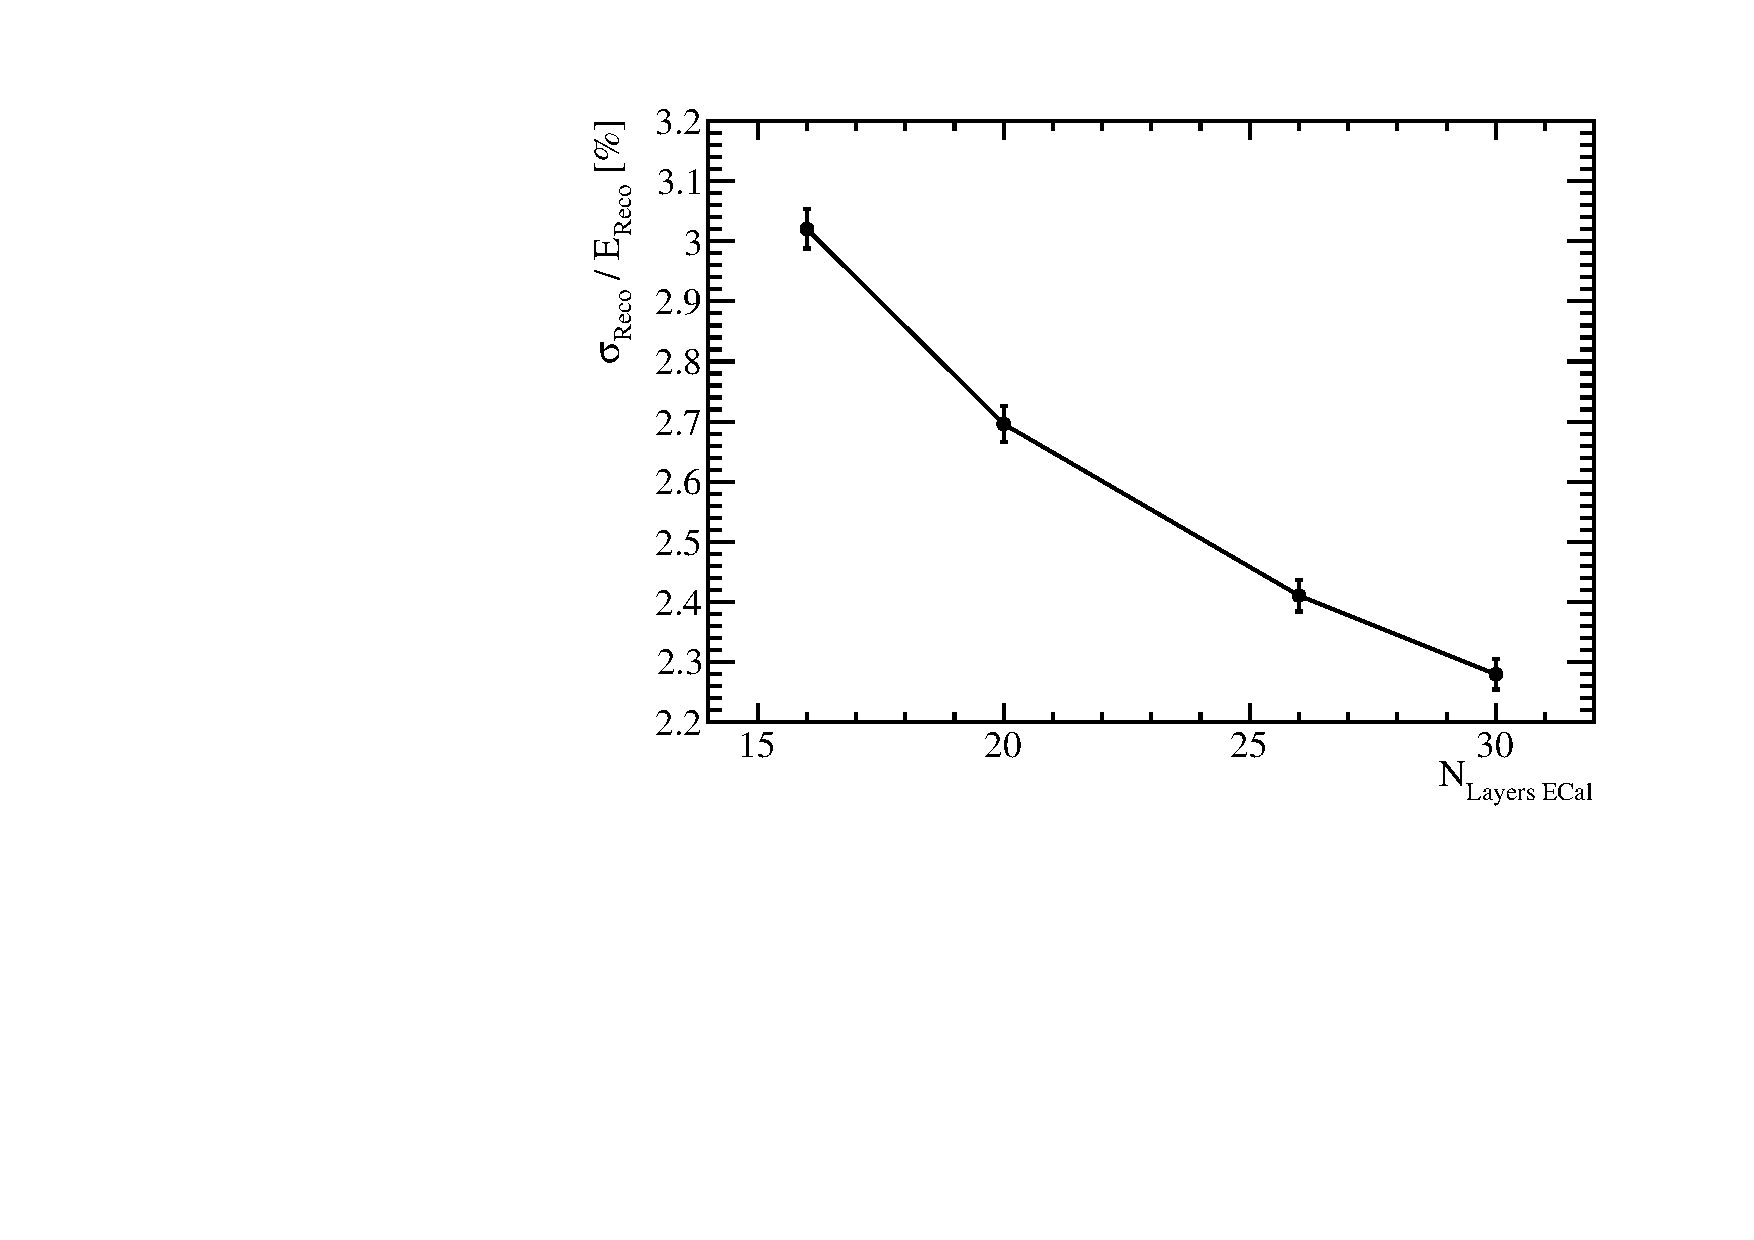
\includegraphics[width=0.5\textwidth]{OptimisationStudies/Plots/EnergyResolution/ER_vs_SiECalNLayers_100GeVPhoton.pdf}}
\subfloat[]{\label{fig:ecalscnlayers100gamma}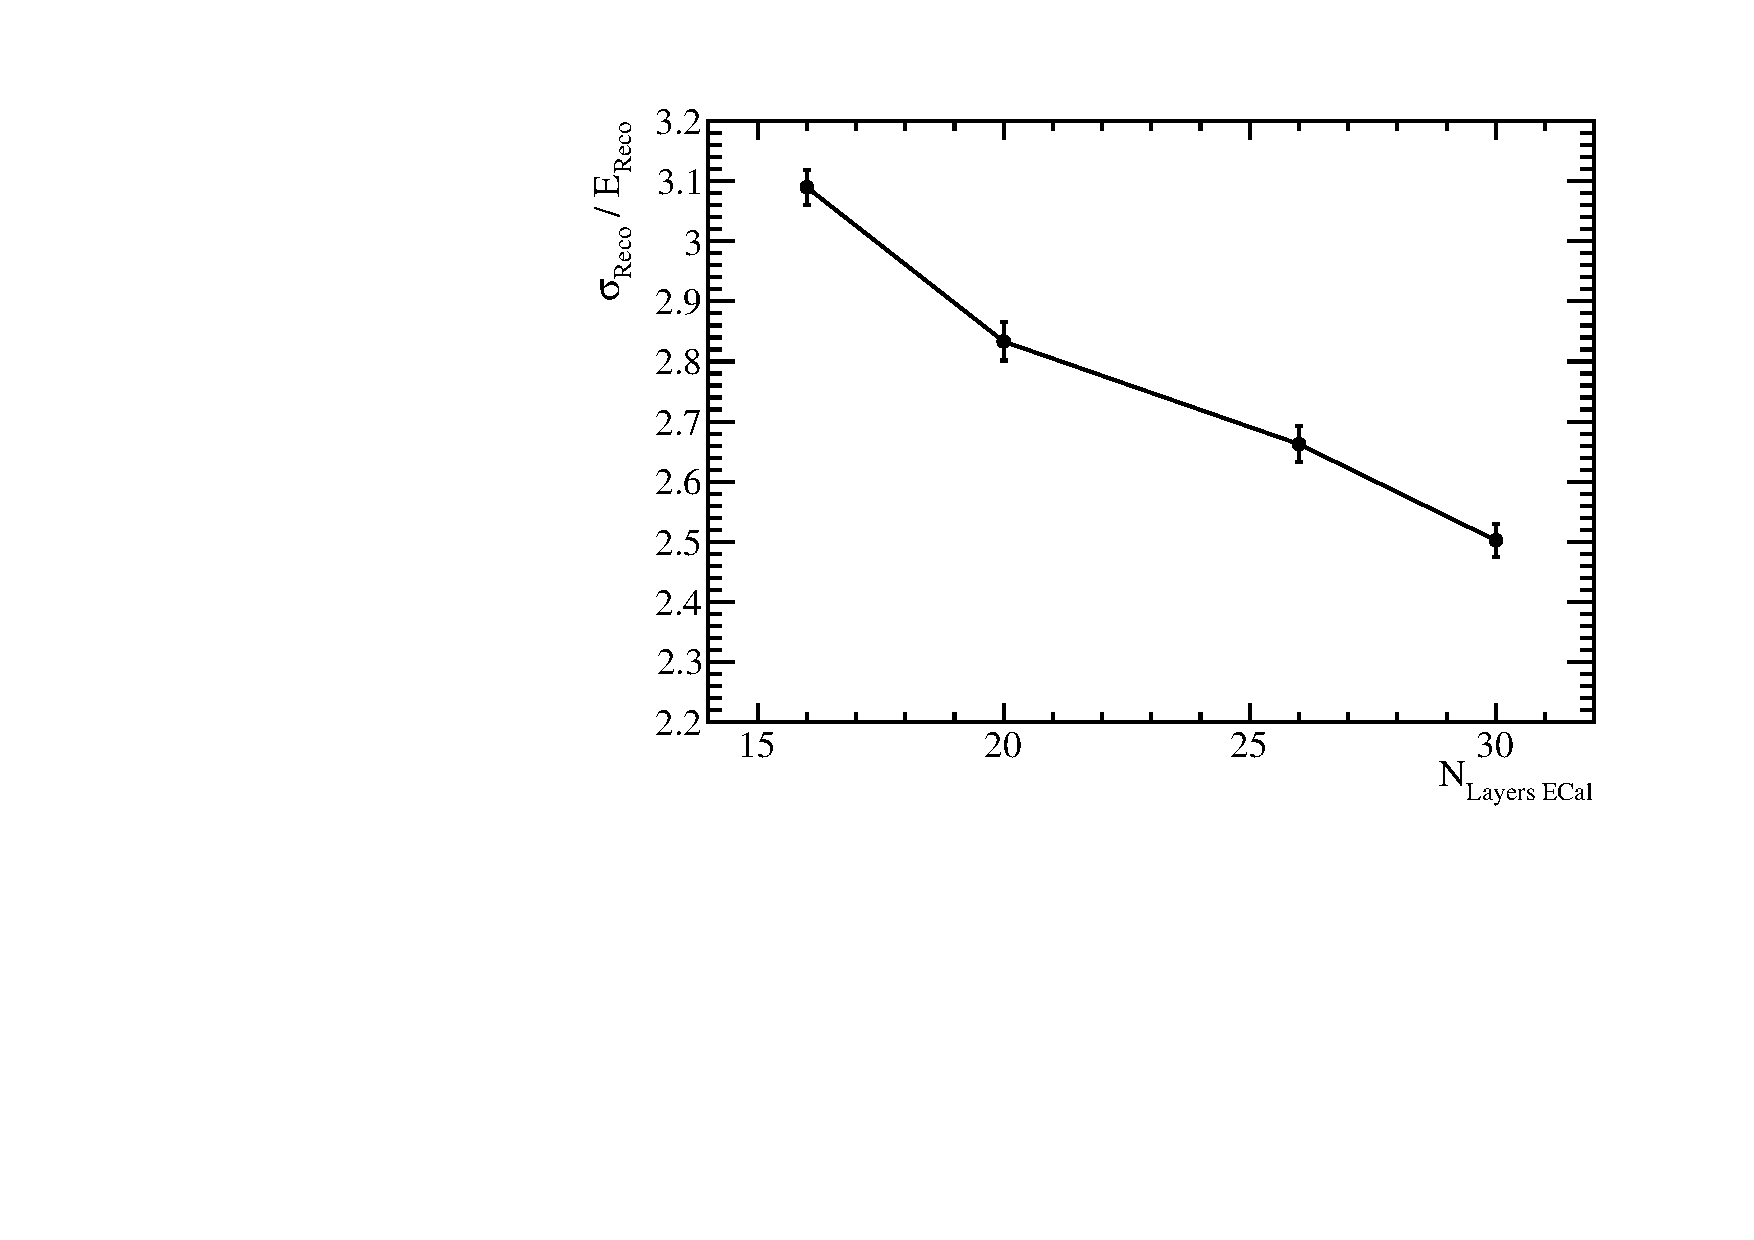
\includegraphics[width=0.5\textwidth]{OptimisationStudies/Plots/EnergyResolution/ER_vs_ScECalNLayers_100GeVPhoton.pdf}}
\caption[The energy resolution as a function of number of layers in the ECal for 100 GeV $\gamma$s using the nominal ILD detector model with \protect\subref{fig:ecalsinlayers100gamma} the silicon and \protect\subref{fig:ecalscnlayers100gamma} the scintillator ECal option.]{The energy resolution as a function of number of layers in the ECal for 100 GeV $\gamma$s using the nominal ILD detector model with \protect\subref{fig:ecalsinlayers100gamma} the silicon and \protect\subref{fig:ecalscnlayers100gamma} the scintillator ECal option.}
\label{fig:ecalnlayersgamma}
\end{figure}

Improving the energy resolution of the calorimeters leads to a reduction in the effect of confusion.  A better energy resolution means more precise comparisons can be made between the energy of a calorimeter hit cluster and the momentum of any charged particle track associated to it.  Comparisons such as these are made by PandoraPFA to determine whether the track cluster associations that have been made are consistent.  If a large discrepancy is observed between the cluster energy and track momenta, the clustering of calorimeter hits is modified until a consistent association can be made.  For more details on this comparison see chapter \ref{chap:pflowandlcdetectors}.  This consistency check vastly reduces the number of errors made when clustering calorimeter hits and associating charged particle tracks to those clusters i.e. the confusion.  Therefore, improving the precision of this consistency check, by improving the energy resolution, reduces the effect of confusion.  

When the number of layers in the ECal is increased, the intrinsic energy resolution of the ECal improves.  This has the knock on effect of reducing the confusion contribution to the jet energy resolution, which can be seen in figure \ref{fig:ecalsinlayers} and \ref{fig:ecalscnlayers} for the silicon and scintillator ECal options respectively.  In both cases the jet energy resolution was found to improve when the number of layers in the ECal is increased.  The magnitude of the change in jet energy resolution was, however, dependent upon the jet energy, with a stronger dependancy being observed for low energy jets.  The origin of this trend will be the stochastic term in the energy resolution for a sampling calorimeter, which is $\propto \frac{1}{\sqrt{E \times N_{Layers}}}$ where $E$ is the reconstructed energy and $N_{Layers}$ is the number of layers in the calorimeter.  At high jet energies, the energy resolution in the ECal is small and changes to the stochastic term that occur when varying the number of layers are too fine to be resolved using jet energy resolution.  While at low jet energies the stochastic term is larger making it possible to resolve the changes to it when varying the number of layers in the ECal.  The jet energy resolution is less sensitive then the single $\gamma$ energy resolution to changes in the number of ECal layers as only $\approx 30\%$ of jet energy is carried in the form of $\gamma$s.  The decomposition of the jet energy resolution into the intrinsic energy resolution and confusion contributions for 45 and 250~GeV jets are shown, for both the silicon and scintillator ECal options, in figure \ref{fig:ecalnlayersbreak}.  As expected, the twofold reduction in both the intrinsic energy resolution and the confusion contribution to the jet energy resolution is observed when increasing the number of layers in the ECal.  Furthermore, changes to both jet energy resolution contributions when varying the number of layers in the ECal are comparable in size indicating that they are both crucial for determining the overall detector performance.  

\begin{figure}[h!]
\centering
\subfloat[]{\label{fig:ecalsinlayers}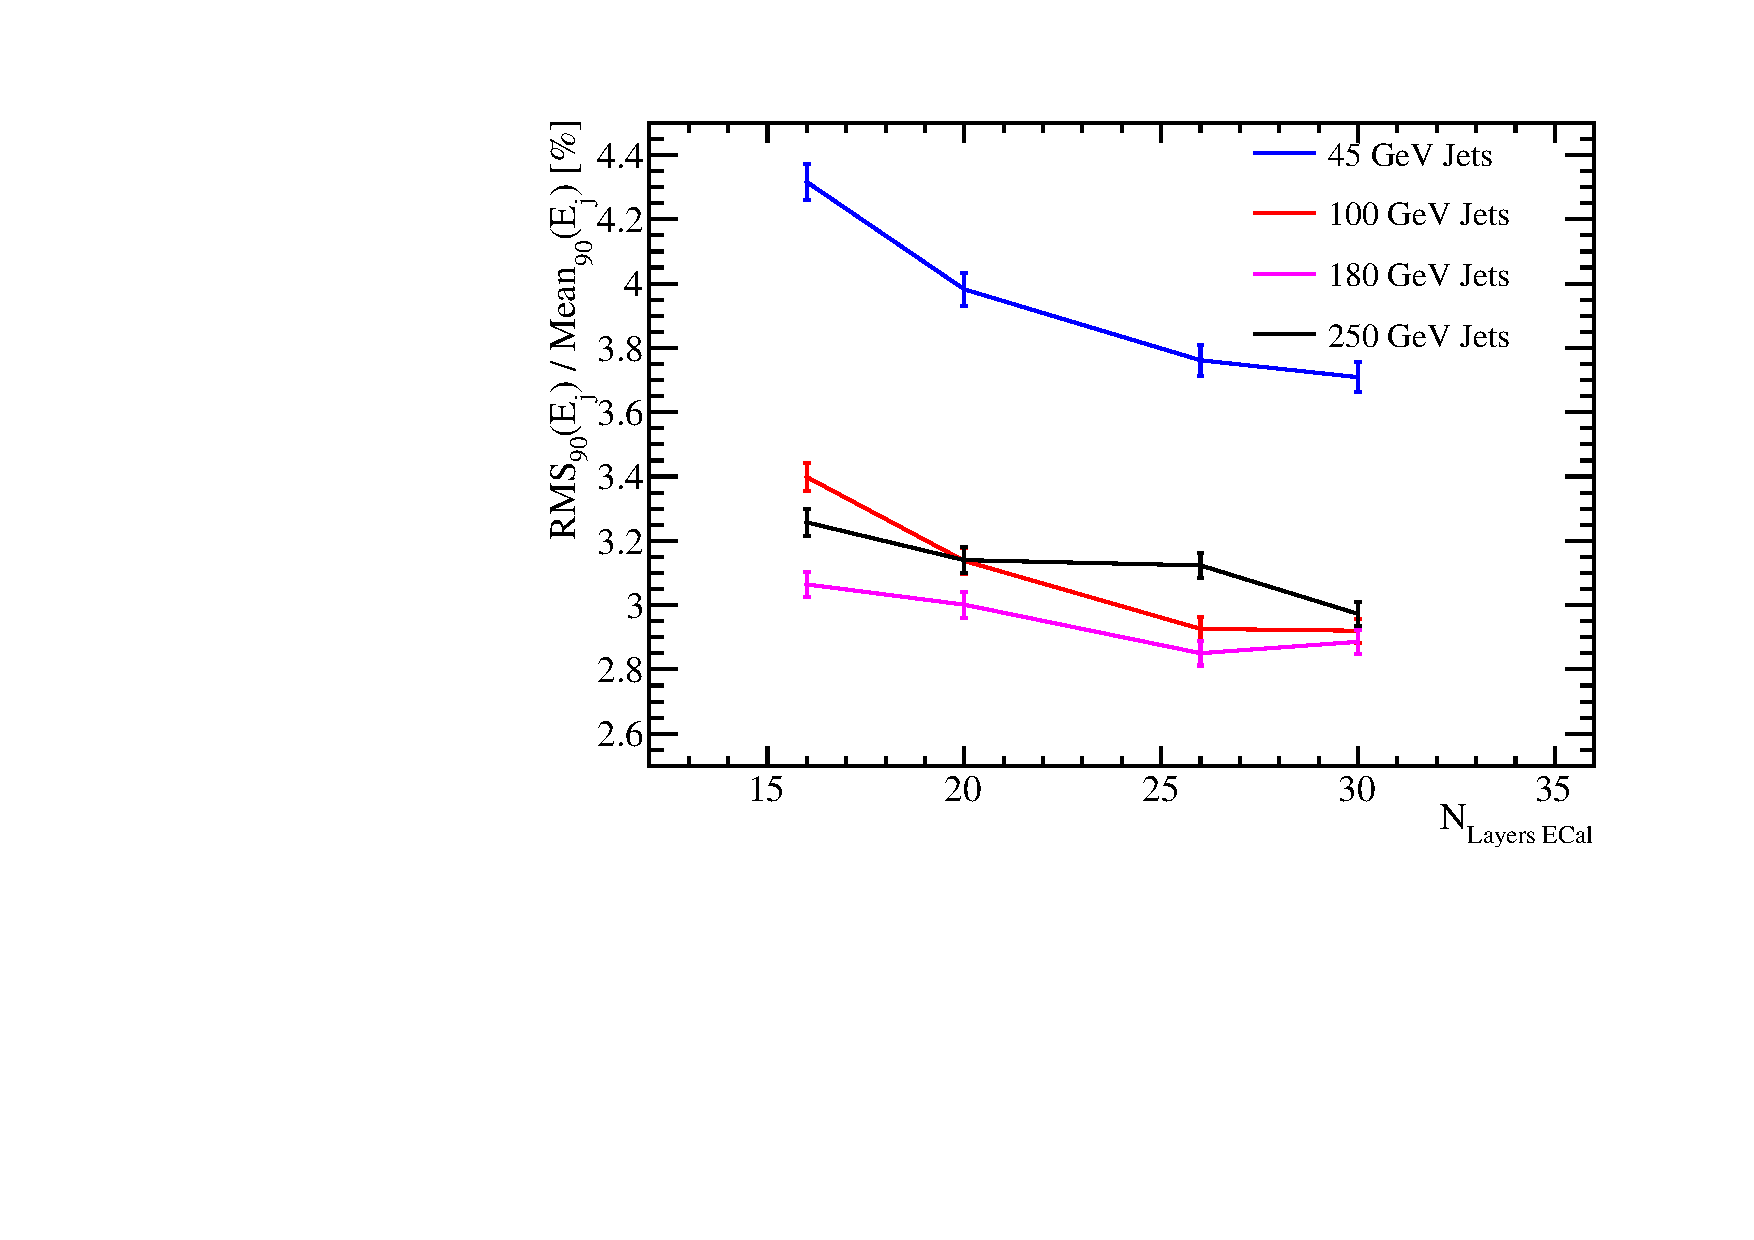
\includegraphics[width=0.5\textwidth]{OptimisationStudies/Plots/JetEnergyResolutions/JER_vs_SiliconECalNumberofLayers.pdf}}
\subfloat[]{\label{fig:ecalscnlayers}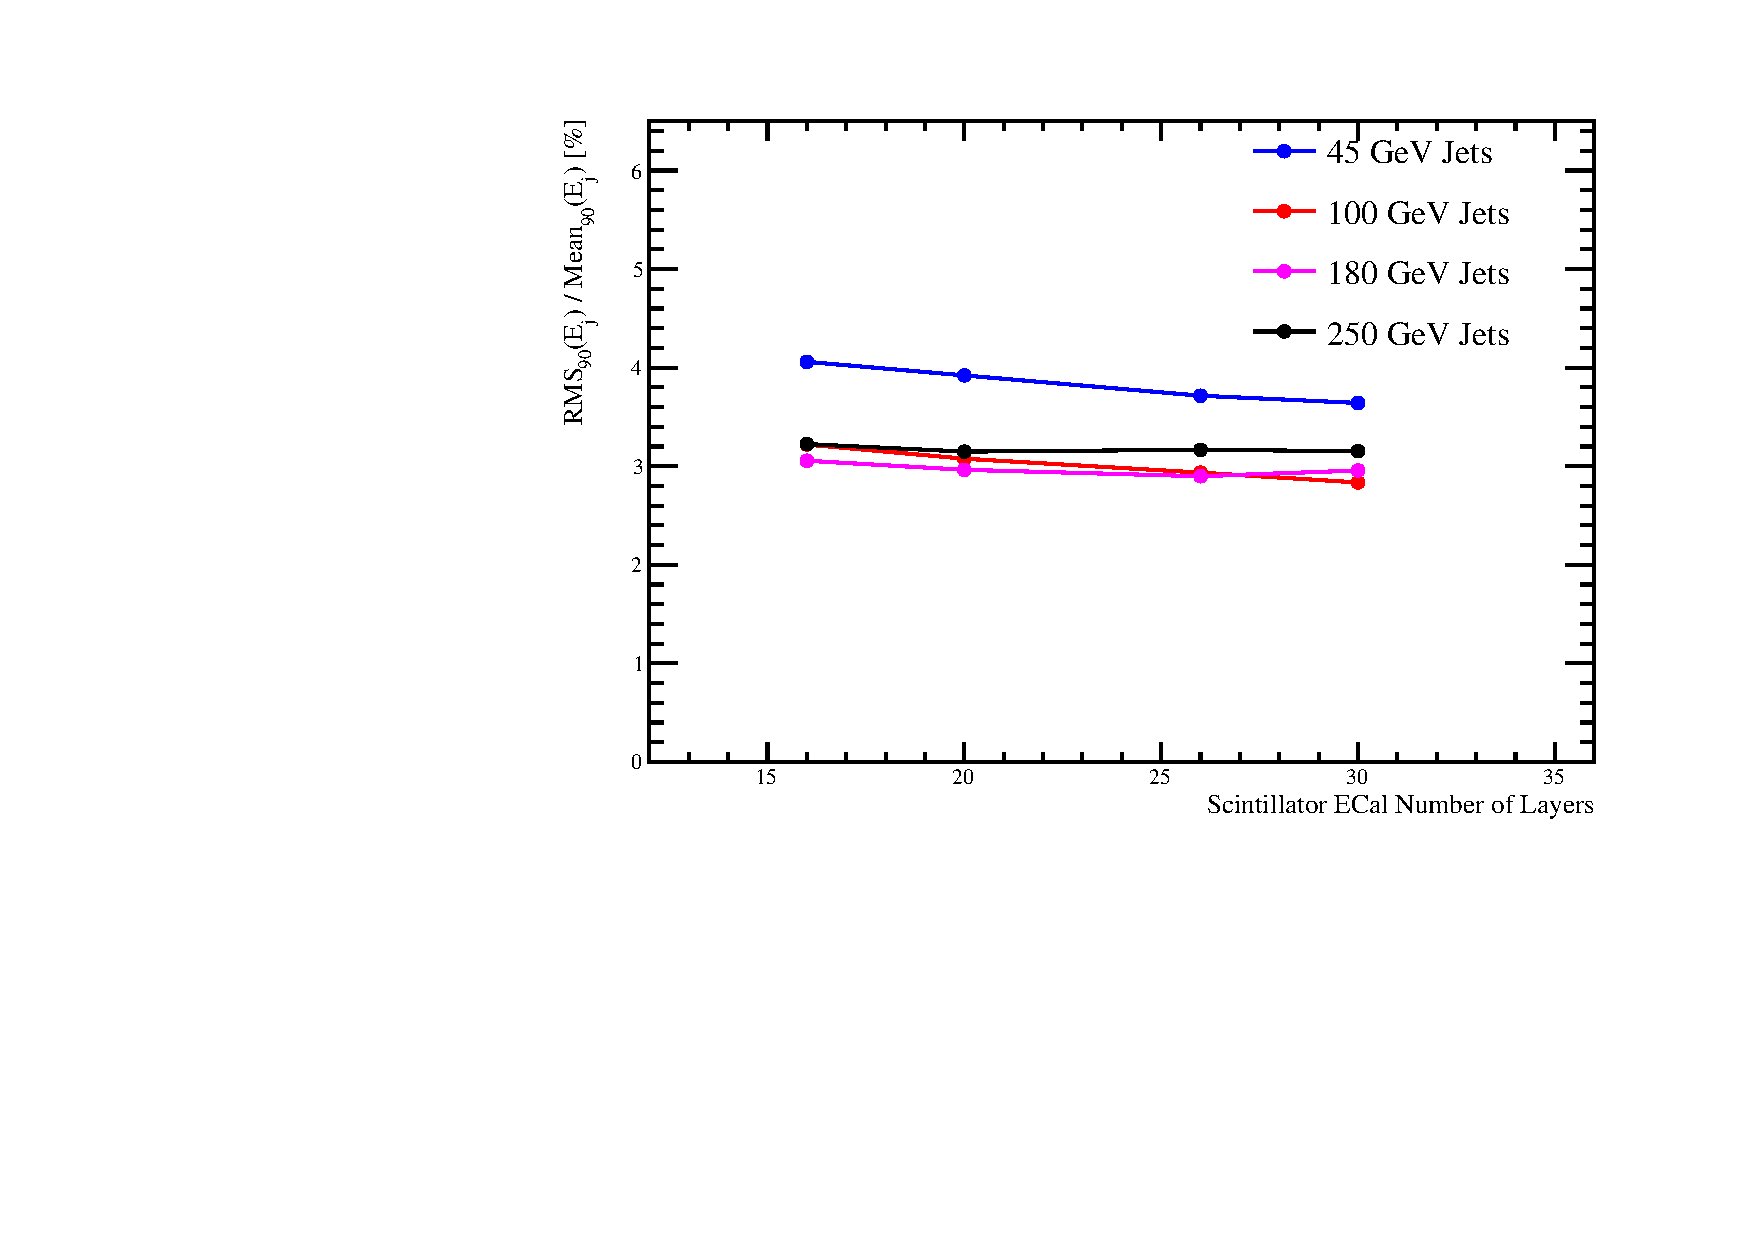
\includegraphics[width=0.5\textwidth]{OptimisationStudies/Plots/JetEnergyResolutions/JER_vs_ScintillatorECalNumberofLayers.pdf}} \hfill
\caption[The jet energy resolution as a function of number of layers in the ECal for various jet energies using the nominal ILD detector model with \protect\subref{fig:ecalsinlayers} the silicon and \protect\subref{fig:ecalscnlayers} the scintillator ECal option.]{The jet energy resolution as a function of number of layers in the ECal for various jet energies using the nominal ILD detector model with \protect\subref{fig:ecalsinlayers} the silicon and \protect\subref{fig:ecalscnlayers} the scintillator ECal option.}
\label{fig:ecalnlayers}
\end{figure}

% MAYBE REMOVE PHOTON CONFUSION
\begin{figure}[h!]
\centering
\subfloat[Silicon active material, 45 GeV Jets.]{\label{fig:ecalsinlayers45break}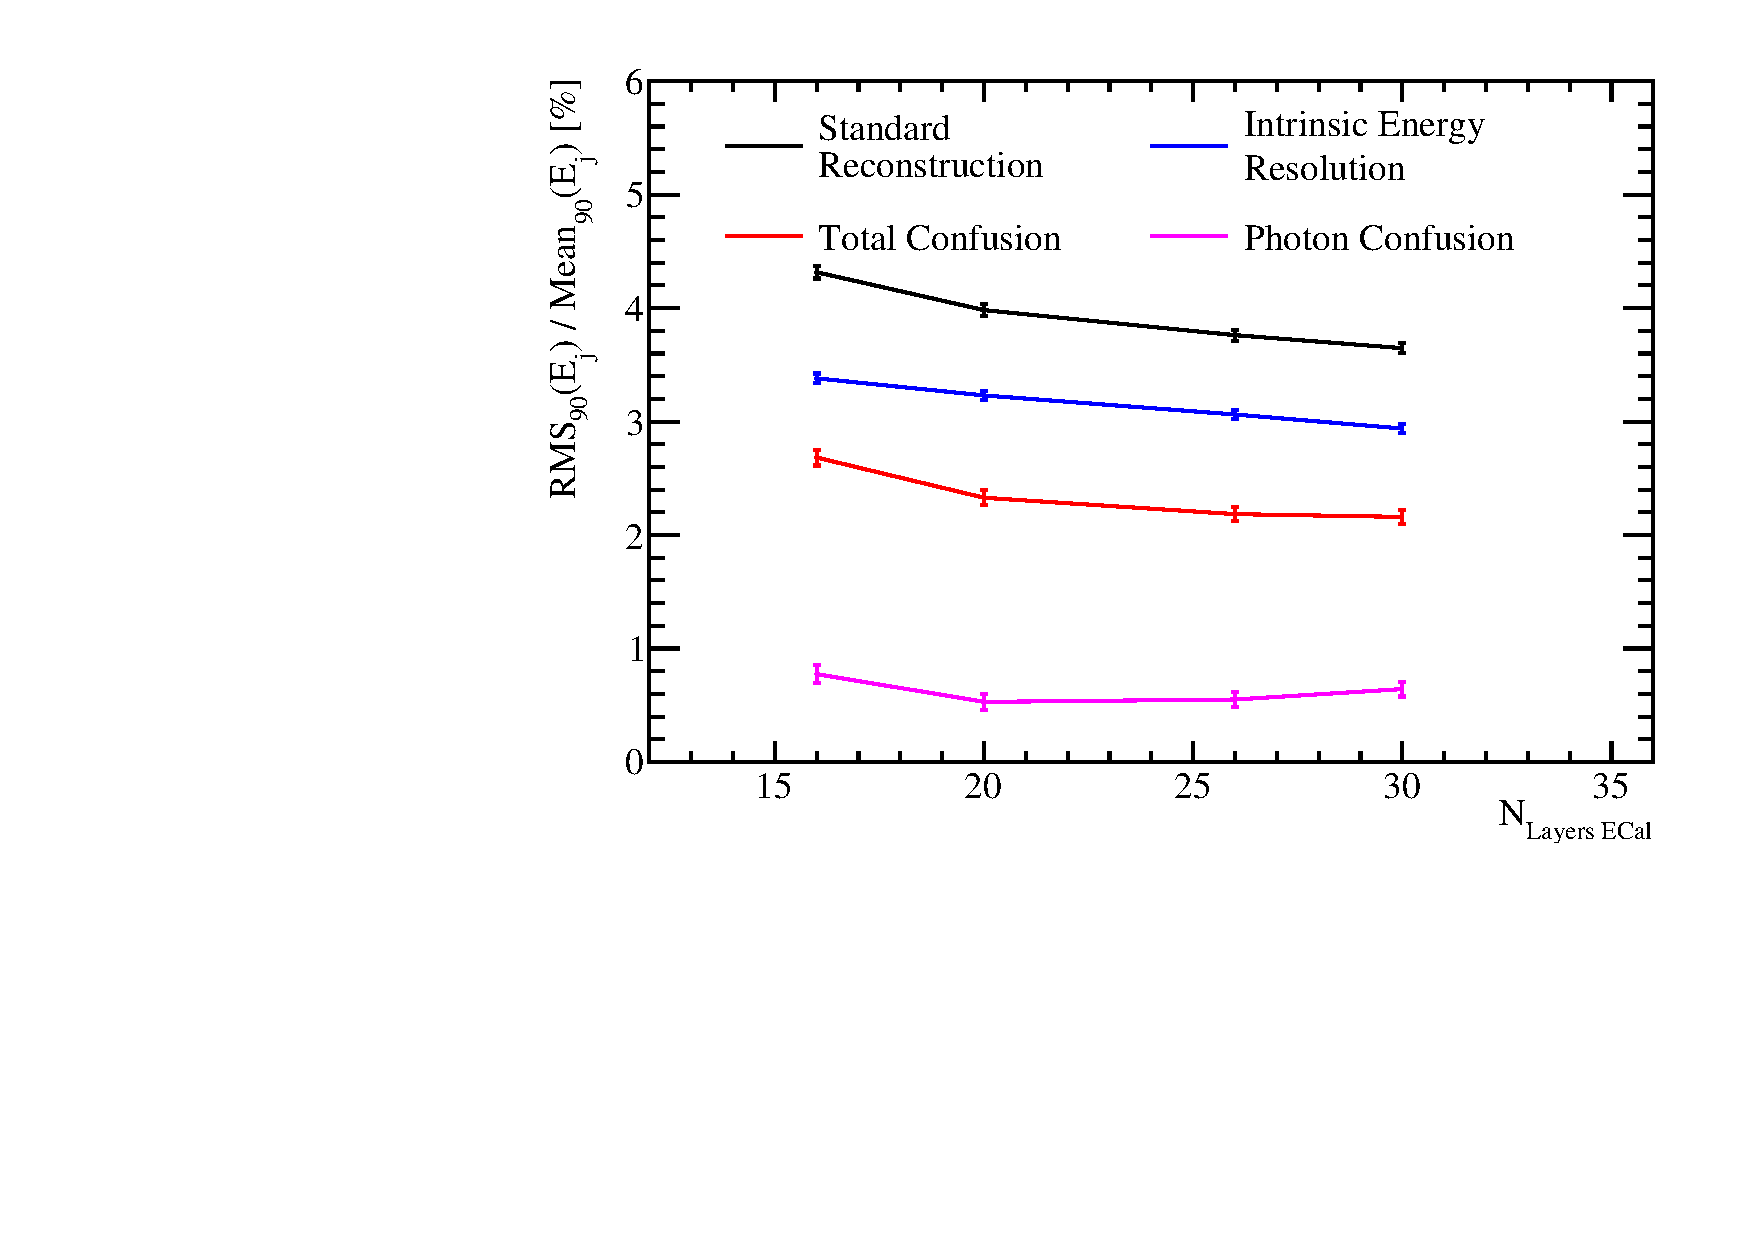
\includegraphics[width=0.5\textwidth]{OptimisationStudies/Plots/JetEnergyResolutions/JER_vs_SiliconECalNumberofLayers_91GeV_DiJet_Breakdown.pdf}}
\subfloat[Scintillator active material, 45 GeV Jets.]{\label{fig:ecalscnlayers45break}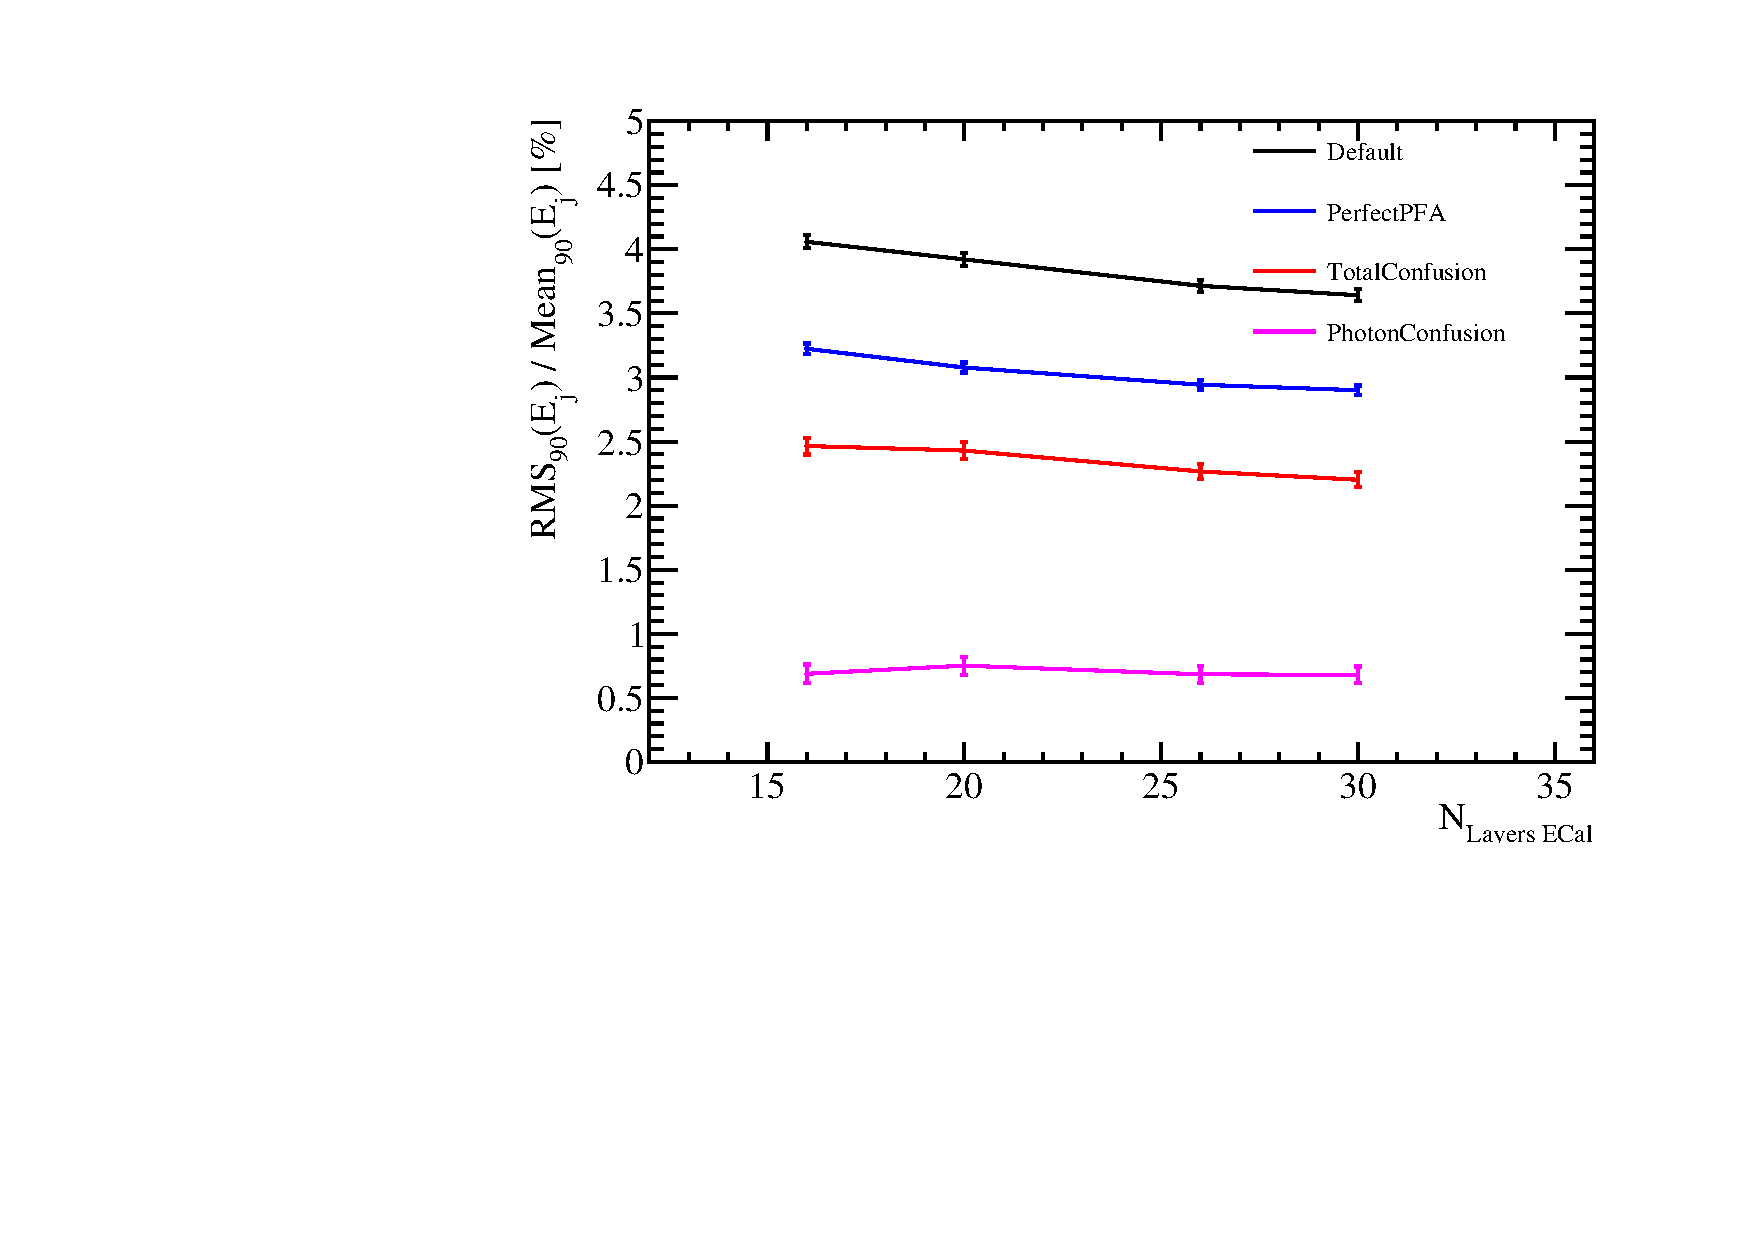
\includegraphics[width=0.5\textwidth]{OptimisationStudies/Plots/JetEnergyResolutions/JER_vs_ScintillatorECalNumberofLayers_91GeV_DiJet_Breakdown.pdf}} \hfill
\subfloat[Silicon active material, 250 GeV Jets.]{\label{fig:ecalsinlayers250break}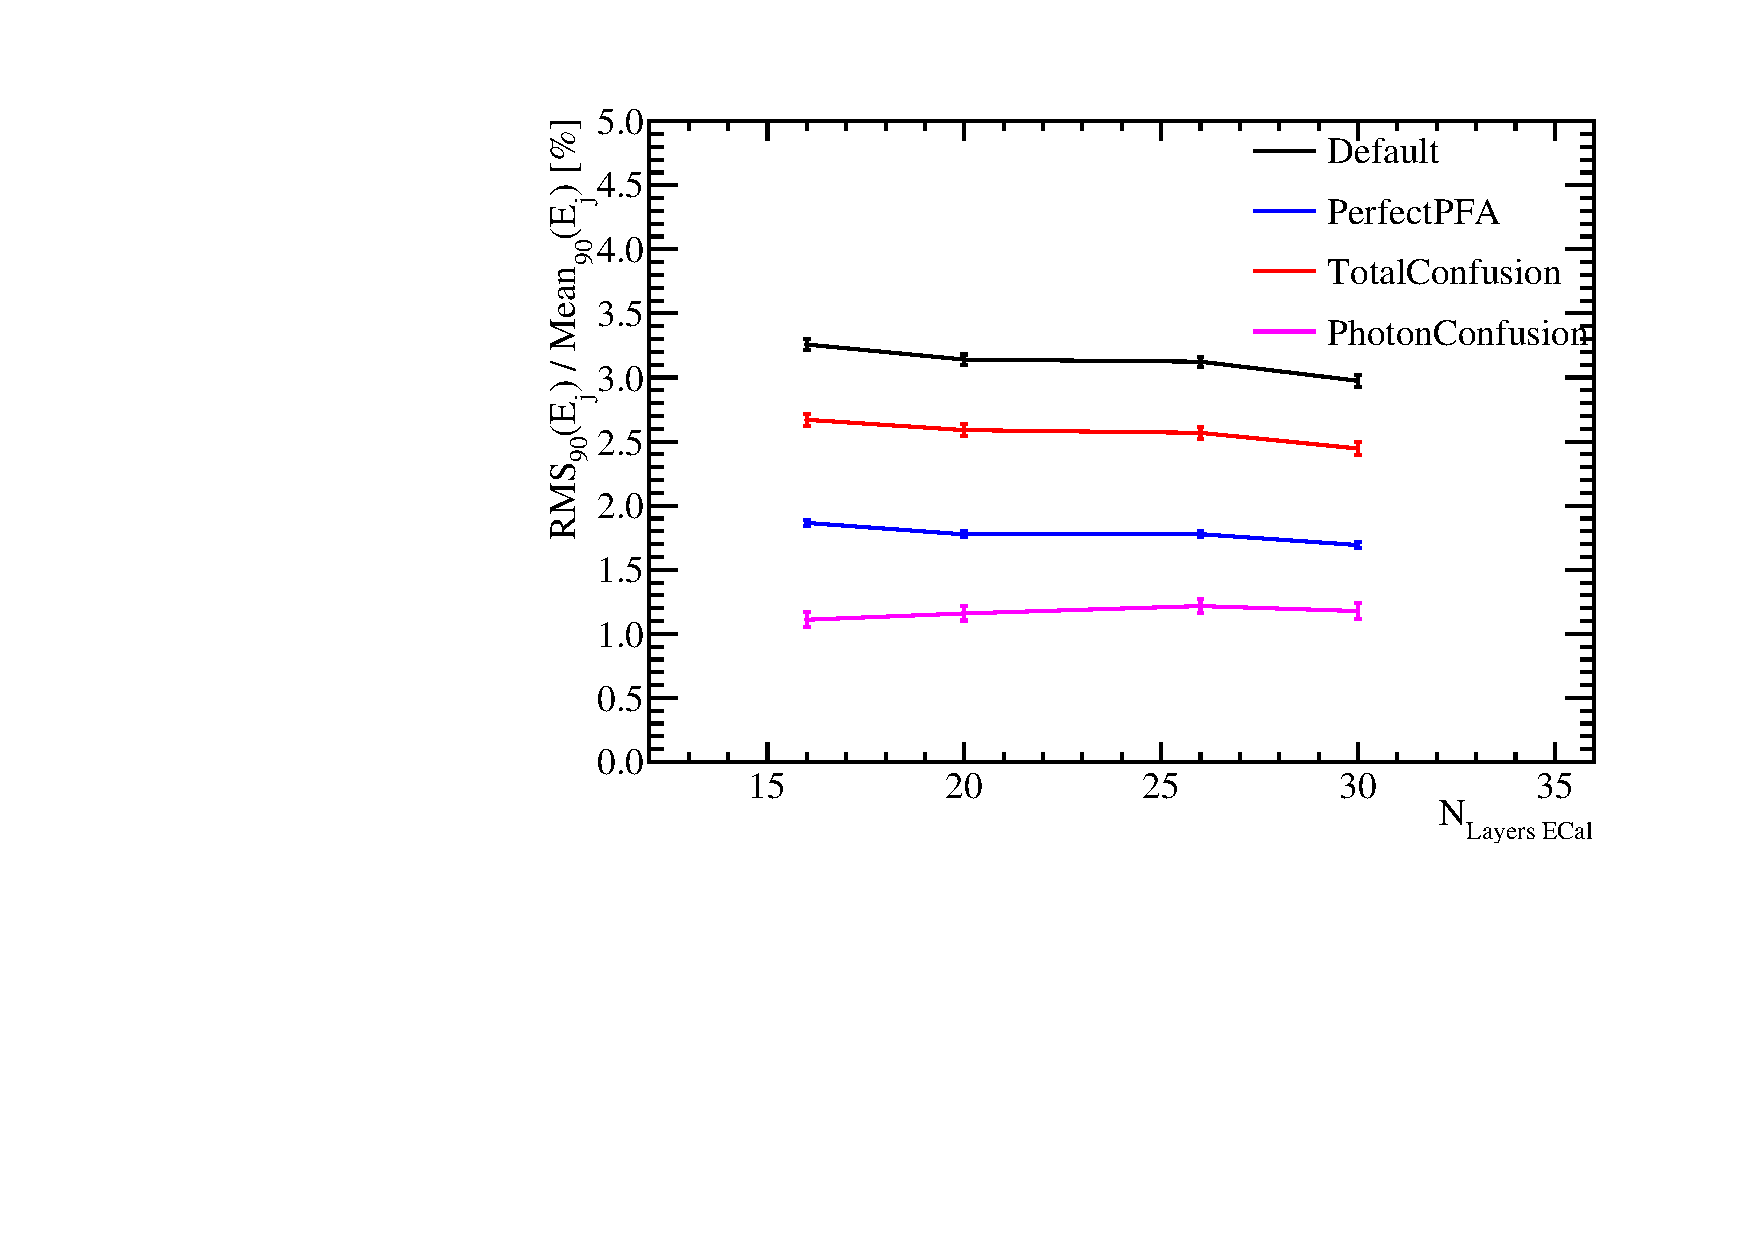
\includegraphics[width=0.5\textwidth]{OptimisationStudies/Plots/JetEnergyResolutions/JER_vs_SiliconECalNumberofLayers_500GeV_DiJet_Breakdown.pdf}}
\subfloat[Scintillator active material, 250 GeV Jets.]{\label{fig:ecalscnlayers250break}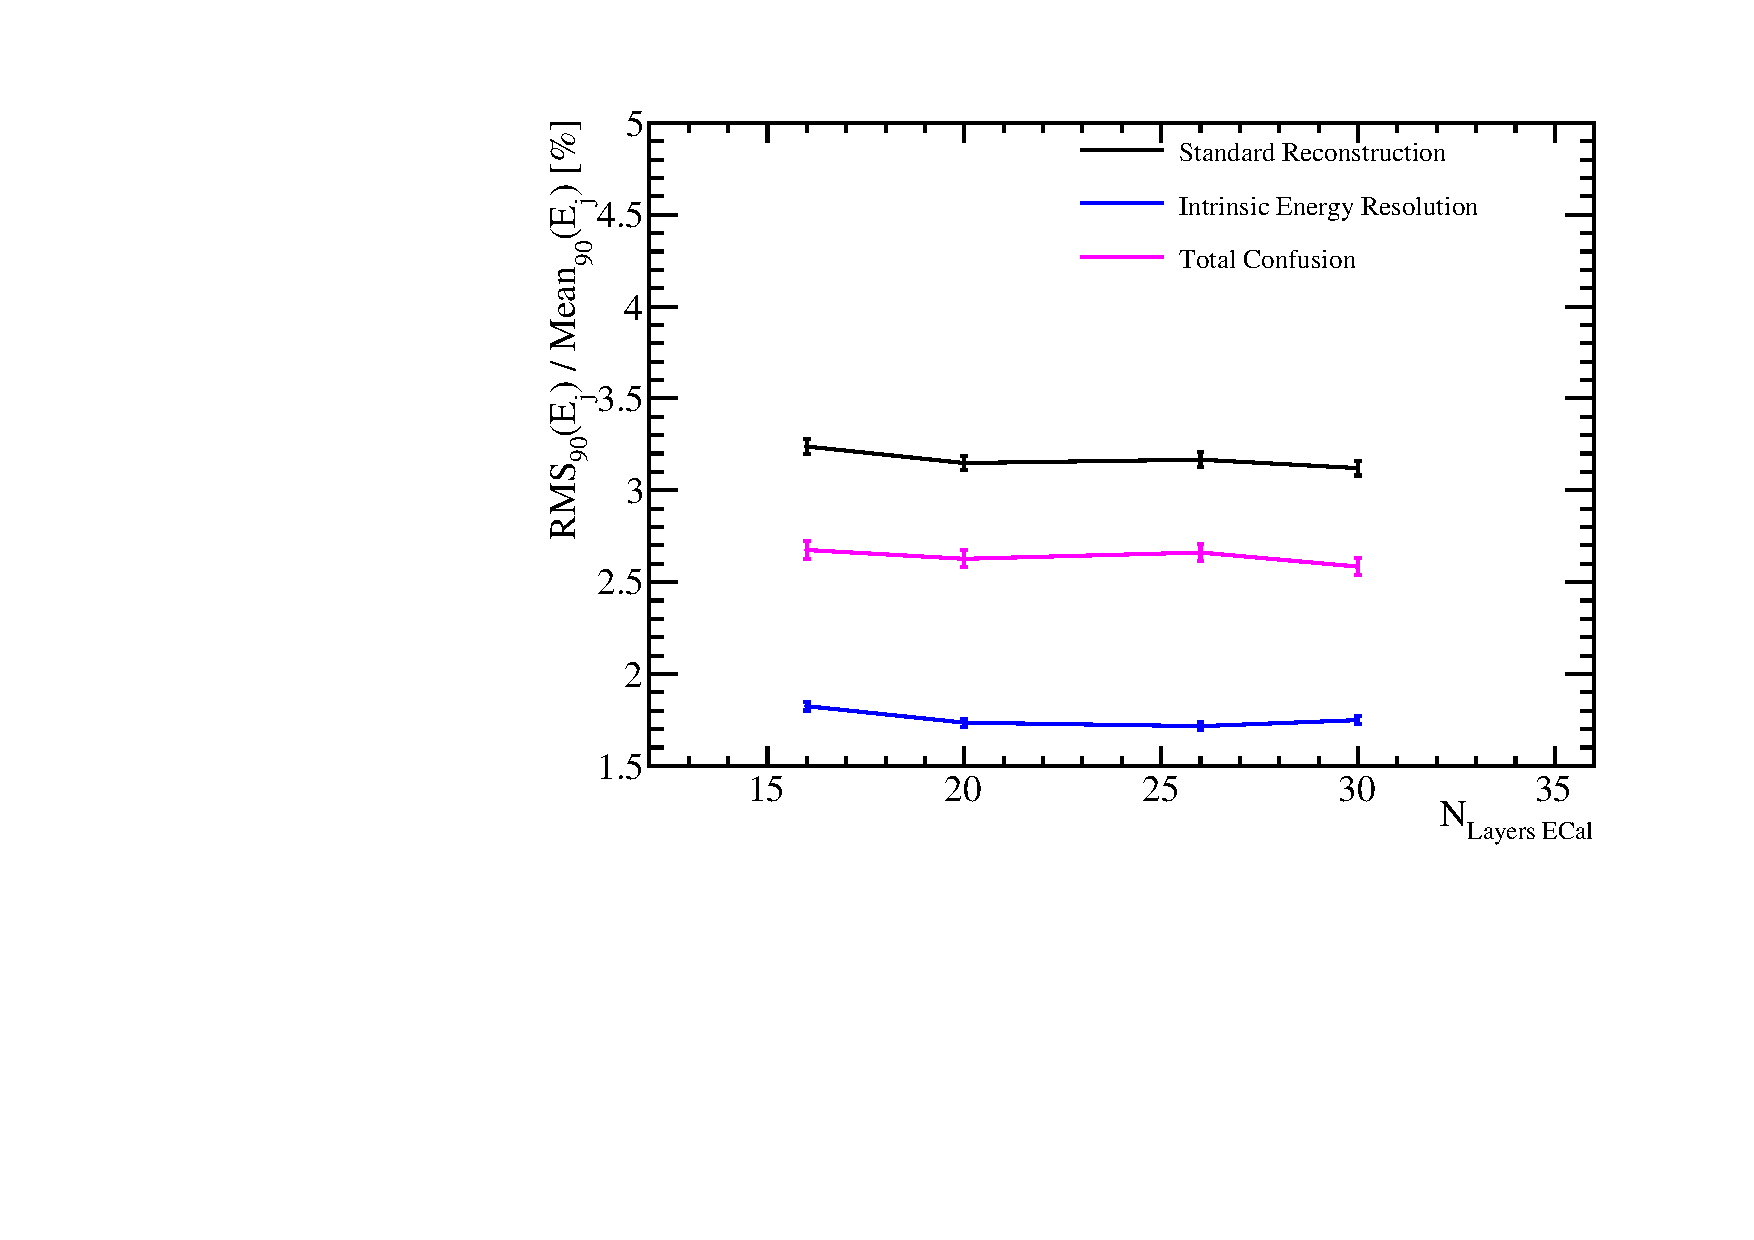
\includegraphics[width=0.5\textwidth]{OptimisationStudies/Plots/JetEnergyResolutions/JER_vs_ScintillatorECalNumberofLayers_500GeV_DiJet_Breakdown.pdf}}
\caption[The contributions to the jet energy resolution as a function of number of layers in the ECal using the nominal ILD detector model for \protect\subref{fig:ecalsinlayers45break} the silicon ECal option and 45 GeV jets, \protect\subref{fig:ecalscnlayers45break} the scintillator ECal option and 45 GeV jets, \protect\subref{fig:ecalsinlayers250break} the silicon ECal option and 250 GeV jets and \protect\subref{fig:ecalscnlayers250break} the scintillator ECal option and 250 GeV jets.  The black curves correspond to the standard reconstruction, the blue curves to the intrinsic energy resolution contribution to the jet energy resolution, the red curves to the confusion contribution to the jet energy resolution and the magenta curves to the confusion contribution to the jet energy resolution related solely to $\gamma$ reconstruction.]{The contributions to the jet energy resolution as a function of number of layers in the ECal using the nominal ILD detector model for \protect\subref{fig:ecalsinlayers45break} the silicon ECal option and 45 GeV jets, \protect\subref{fig:ecalscnlayers45break} the scintillator ECal option and 45 GeV jets, \protect\subref{fig:ecalsinlayers250break} the silicon ECal option and 250 GeV jets and \protect\subref{fig:ecalscnlayers250break} the scintillator ECal option and 250 GeV jets.  The black curves correspond to the standard reconstruction, the blue curves to the intrinsic energy resolution contribution to the jet energy resolution, the red curves to the confusion contribution to the jet energy resolution and the magenta curves to the confusion contribution to the jet energy resolution related solely to $\gamma$ reconstruction.}
\label{fig:ecalnlayersbreak}
\end{figure}

Increasing the number of layers in the ECal is beneficial to the intrinsic energy resolution of the ECal as well as the jet energy resolution, particularly for low jet energies.  Separation of the W and Z hadronic decays should be possible for ILC like energies given there are at least 26 layers in the ECal, however, it is desirable to have as large a number of layers as possible to benefit single $\gamma$ energy resolution also.  

%========================================================================================

\subsection{ECal Active Material}
In sections \ref{sec:ecalcells} and \ref{sec:ecalnlayers} the performance of the ECal was reported for both the silicon and scintillator options and to a large extent the performance of the two options was similar, but not identical:

\begin{itemize}
\item The intrinsic energy resolution of the silicon ECal option is better than that of a scintillator option for high energies, see figures \ref{fig:ecalsinominalres} and \ref{fig:ecalscnominalres}.  This is most likely due to the implementation of Birks' law \cite{BirksLaw} for scintillator active materials.  Birks' law states:
\begin{equation}
\frac{d\mathcal{L}}{dx} \propto \times \frac{dE/dx}{1+k_{B}dE/dx}\text{ ,}
\end{equation}
where $\frac{d\mathcal{L}}{dx}$ is the light yield per unit path length, $dE/dx$ is the energy deposited per unit path length and $k_{B}$ is a material property constant.  For large energy deposits per unit length, such as those found in high energy $\gamma$ events, the light yield saturates causing a degradation in the energy resolution.  Based on a comparison with the silicon ECal option performance, this effect starts to degrade the energy resolution for the scintillator option around ~50 GeV.  However, the degradation in energy resolution up to 100 GeV is relatively small.
\item The "dead" region due to the presence of the MPPC in the simulation of the scintillator ECal option degrades performance of the detector for small transverse granularities, see figure \ref{fig:ecalcellsizegamma}.
\end{itemize}

In summary, the performance of the two options in terms of energy and jet energy resolution are similar, meaning no clear option is preferred.  However, the silicon option is preferred when manufacture and implementation of the two models is compared.  While constructing silicon wafers to fit the $5 \times 5 \text{mm}^{2}$ square cell size of the ECal is achievable, this would be extremely challenging for scintillator tiles.  To resolve this in actuality, the scintillator ECal option would have to use $5 \times 45 \text{mm}^{2}$ scintillator strips that are arranged in alternating directions in each ECal layer.  By combining information from neighbouring layers it becomes possible to effectively achieve a $5 \times 5 \text{mm}^{2}$ square cell size.  This further challenge to the reconstruction make the silicon option is the more preferred ECal option.  

%========================================================================================
%========================================================================================

\section{Hadronic Calorimeter Optimisation}
The HCal primarily measures energy deposits from hadronic showers.  The HCal in the default ILD detector model, summarised in table \ref{table:defaultildhcal}, is approximately 6 nuclear interaction lengths ($\lambda_{I}$) deep.  The ECal contributes approximately one $\lambda_{I}$ giving a total of $\approx 7 \lambda_{I}$, which is sufficient to confine the bulk of jets up to 1 TeV events.  The longitudinal structure of this model consists of 48 readout layers each containing a 3 mm active layer of scintillator and a 20 mm absorber layer of iron.  

\begin{table}[h!]
\centering
\begin{tabular}{ l l}
\hline
Parameter & Default Value \\
\hline
Cell Size & $30 \times 30 \text{mm}^{2}$ square cells \\
Number of Layers & 48 readout layers \\
Active Material Choice & Scintillator \\
Active Material Thickness & 3 mm  \\
Absorber Material Choice & Steel \\
Absorber Material Thickness & 20 mm \\
\hline
\end{tabular}
\caption[The configuration of the HCal in the nominal ILD detector model.]{The configuration of the HCal in the nominal ILD detector model.}
\label{table:defaultildhcal}
\end{table}
% Nuclear interaction length iron 167.7mm
% Nuclear interaction length tungsten 99.46mm 
% Nuclear interaction length silicon 465.2mm 
% Nuclear interaction length polystyrene 770.7mm

There are several readout approaches under consideration for the HCal including fully analogue, fully digital and semi-digital.  The analogue readout measures the energy within each HCal cell using a continuous spectrum of measurements, while the digital readout only produces a response if the energy deposited within a calorimeter cell is above a given threshold.  The semi-digital approach mirrors that of the digital approach, but has three responses each with a different energy threshold.  While the energy resolution for digital calorimeters is not as good as that of analogue calorimeters, it is possible to construct smaller cell sizes using a digital readout.  In traditional calorimetry, a digital readout would lead to worsening jet energy resolution, however, that is not necessarily the case in particle flow calorimetry.  If a digital readout could be realised with significantly smaller cell sizes than the analogue equivalent, then the effect of confusion may be reduced enough to compensate for the reduced intrinsic energy resolution.  Therefore, in the following studies only the analogue HCal is considered.

The HCal performance for single hadrons and the overall jet energy resolution will depend on the details of the HCal design.  A number of options were simulated where the following parameters were varied:
\begin{itemize}
\item Cell size:  This is key to successful application of pattern recognition in the particle flow paradigm, but should not change the intrinsic energy resolution.   
\item Number of layers, keeping the absorber and active layers thicknesses constant:  This changes the total depth of the HCal and so will determine the effect of leakage of energy out of the back of the HCal.
\item The sampling frequency:  This involved changing the number of readout layers in the HCal while modifying the thicknesses of the active and absorber layers to keep the total number of nuclear interaction lengths constant.  As this modifies the sampling of particle showers in the HCal it will affect the intrinsic energy resolution.
\item Sampling fraction:  This is the ratio of the active medium thickness to the absorber medium thickness.  This controls how particle showers within the calorimeter are sampled.
\item Absorber material choice:  Two options have been considered: steel and tungsten.  This choice dictates the growth and propagation of hadronic showers and so plays a crucial role in calorimetry.  
\end{itemize}

%========================================================================================

\subsection{HCal Cell Size}
\label{sec:hcalcells}
The HCal cell size is an important detector parameter in the application of particle flow calorimetry.  

Smaller HCal cell sizes will lead to a finer spatial resolution that can be used to better separate charged and neutral particle calorimetric energy deposits.  On the other hand, this will also lead to an increase in the number of readout channels that will raise the cost of the calorimeter.  Therefore, it is highly desirable to achieve the optimal physics performance using the largest cell size possible.  The nominal ILD HCal has a 30 mm square cell size and in this study the following square cell sizes were considered; 10 mm, 20 mm, 30 mm, 40 mm, 50 mm and 100 mm.  

The energy resolution for 50 GeV $\text{K}^{0}_{L}$ events as a function of cell size in the HCal is shown in figure \ref{fig:hcalcellser}.  These $\text{K}^{0}_{L}$ samples will deposit energy primarily within the HCal, making them appropriate events to consider when determining the performance of the HCal.  However, a non-neglibile amount of energy will also be deposited within the ECal.  Therefore, these energy resolutions represent the intrinsic energy resolution of the ILD detector as a whole and not purely that of the HCal.  It is clear that there is no strong dependency on the energy resolution of the $\text{K}^{0}_{L}$ as a function of the HCal cell size.  There are small fluctuations in the energy resolution that are most likely due to variations in applying the calibration procedure and the tuning of the optimal HCal cell truncation, described in section \ref{sec:hcalcelltruncation}.  The precision on the optimal cell truncation is worse for large HCal cell sizes as the truncations considered in the optimisation are focused around the optimal truncation for the nominal ILD HCal.  

\begin{figure}[h!]
\centering
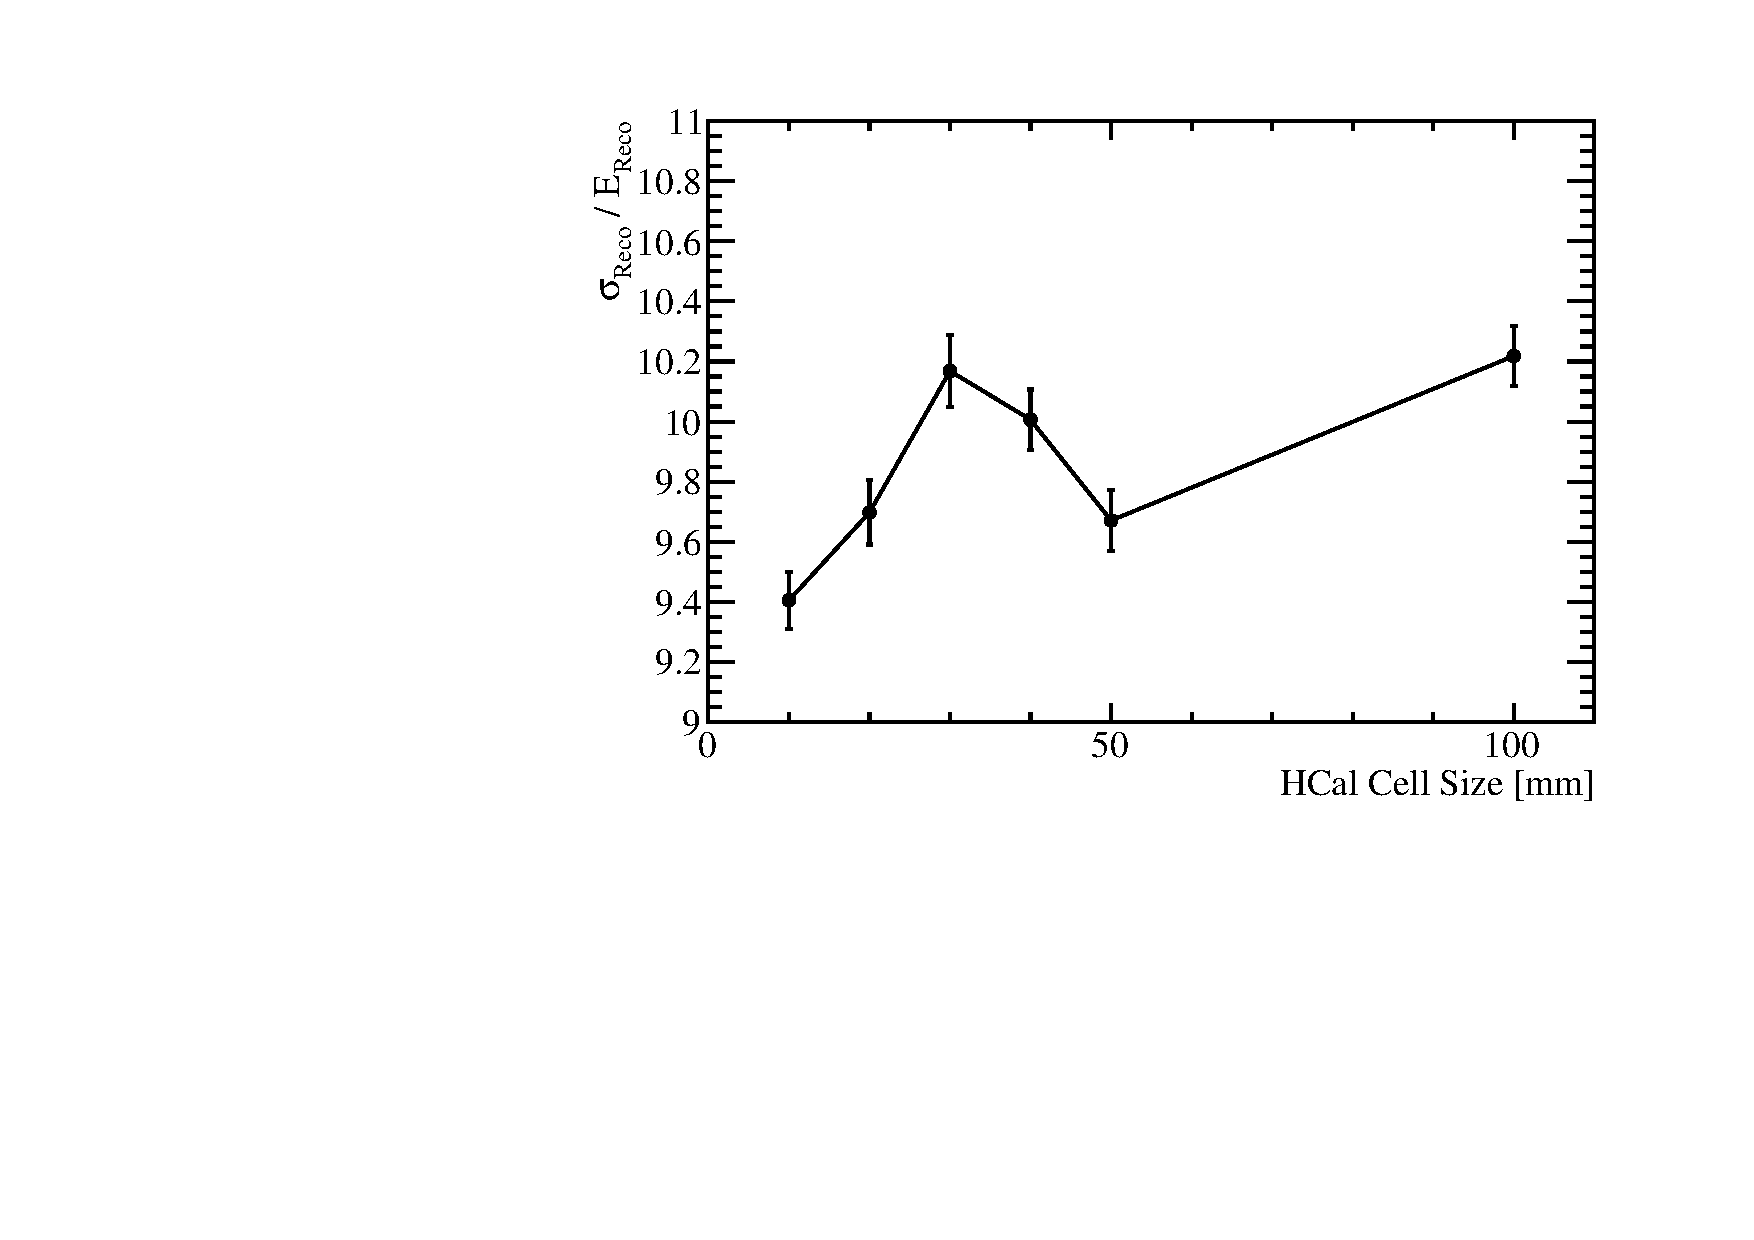
\includegraphics[width=0.5\textwidth]{OptimisationStudies/Plots/EnergyResolution/ER_vs_HCalCellSize_50GeVKaon0L.pdf}
\caption[The energy resolution as a function of HCal cell size for 50 GeV $\text{K}^{0}_{L}$ events using the nominal ILD detector model.]{The energy resolution as a function of HCal cell size for 50 GeV $\text{K}^{0}_{L}$ events using the nominal ILD detector model.}
\label{fig:hcalcellser}
\end{figure}

As a smaller HCal cell size will lead to better separation of charged and neutral hadron calorimetric energy deposits, it is expected that the confusion contribution to the jet energy resolution will be reduced by using smaller HCal cell sizes.  The jet energy resolution as a function of cell size in the HCal shown in figure \ref{fig:hcalcellsize}.  At low jet energies there is no strong dependency of the jet energy resolution on the HCal cell size, which is as expected from the $\text{K}^{0}_{L}$ energy resolution study.  For high energy jets there is a clear dependence, with lower HCal cell sizes leading to better jet energy resolutions.  Examining the different contributions to the jet energy resolution, shown in figure \ref{fig:hcalcellsizebreak} it can be seen that the intrinsic energy resolution contribution is largely invariant to changes in the HCal cell size.  Instead it is the confusion contribution that drives the overall trend in the jet energy resolution.  This is particularly clear at high jet energies where the confusion contribution to the jet energy resolution dominates that of the intrinsic energy resolution contribution.  The confusion contribution does fluctuate for small HCal cell sizes when considering low jet energies, but this will be due to tuning of the PandoraPFA algorithms to the nominal ILD HCal cell size.  As the confusion contribution is not dominant at low energies, this effect is masked when considering the jet energy resolution metric.  Furthermore, as the photon confusion is largely invariant to changes in the HCal cell size it indicates that the confusion contribution is changing due to pattern recognition improvements related to charged and neutral hadrons.

\begin{figure}[h!]
\centering
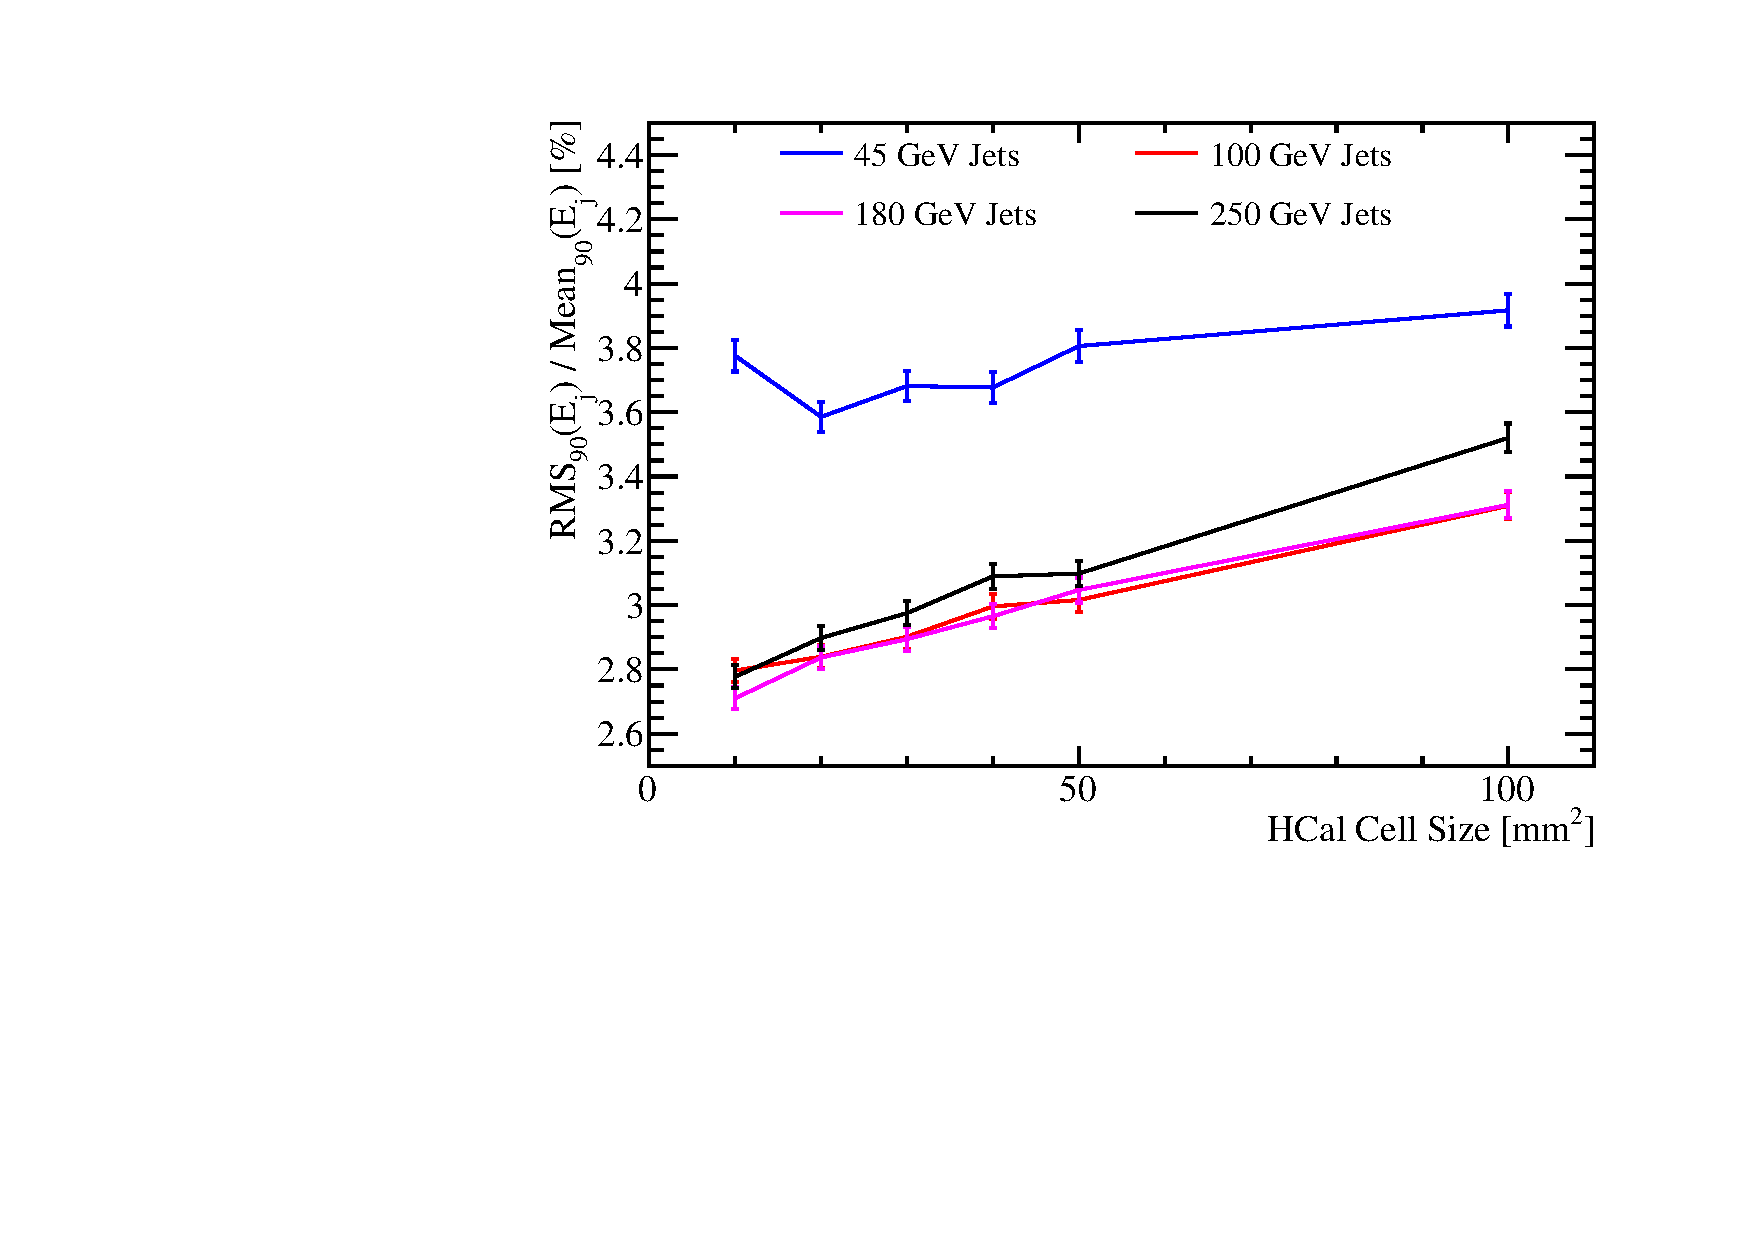
\includegraphics[width=0.5\textwidth]{OptimisationStudies/Plots/JetEnergyResolutions/JER_vs_HCalCellSize.pdf}
\caption[The jet energy resolution as a function of HCal cell size for various jet energies using the nominal ILD detector model.]{The jet energy resolution as a function of HCal cell size for various jet energies using the nominal ILD detector model.}
\label{fig:hcalcellsize}
\end{figure}

\begin{figure}[h!]
\centering
\subfloat[]{\label{fig:hcalcellsize45break}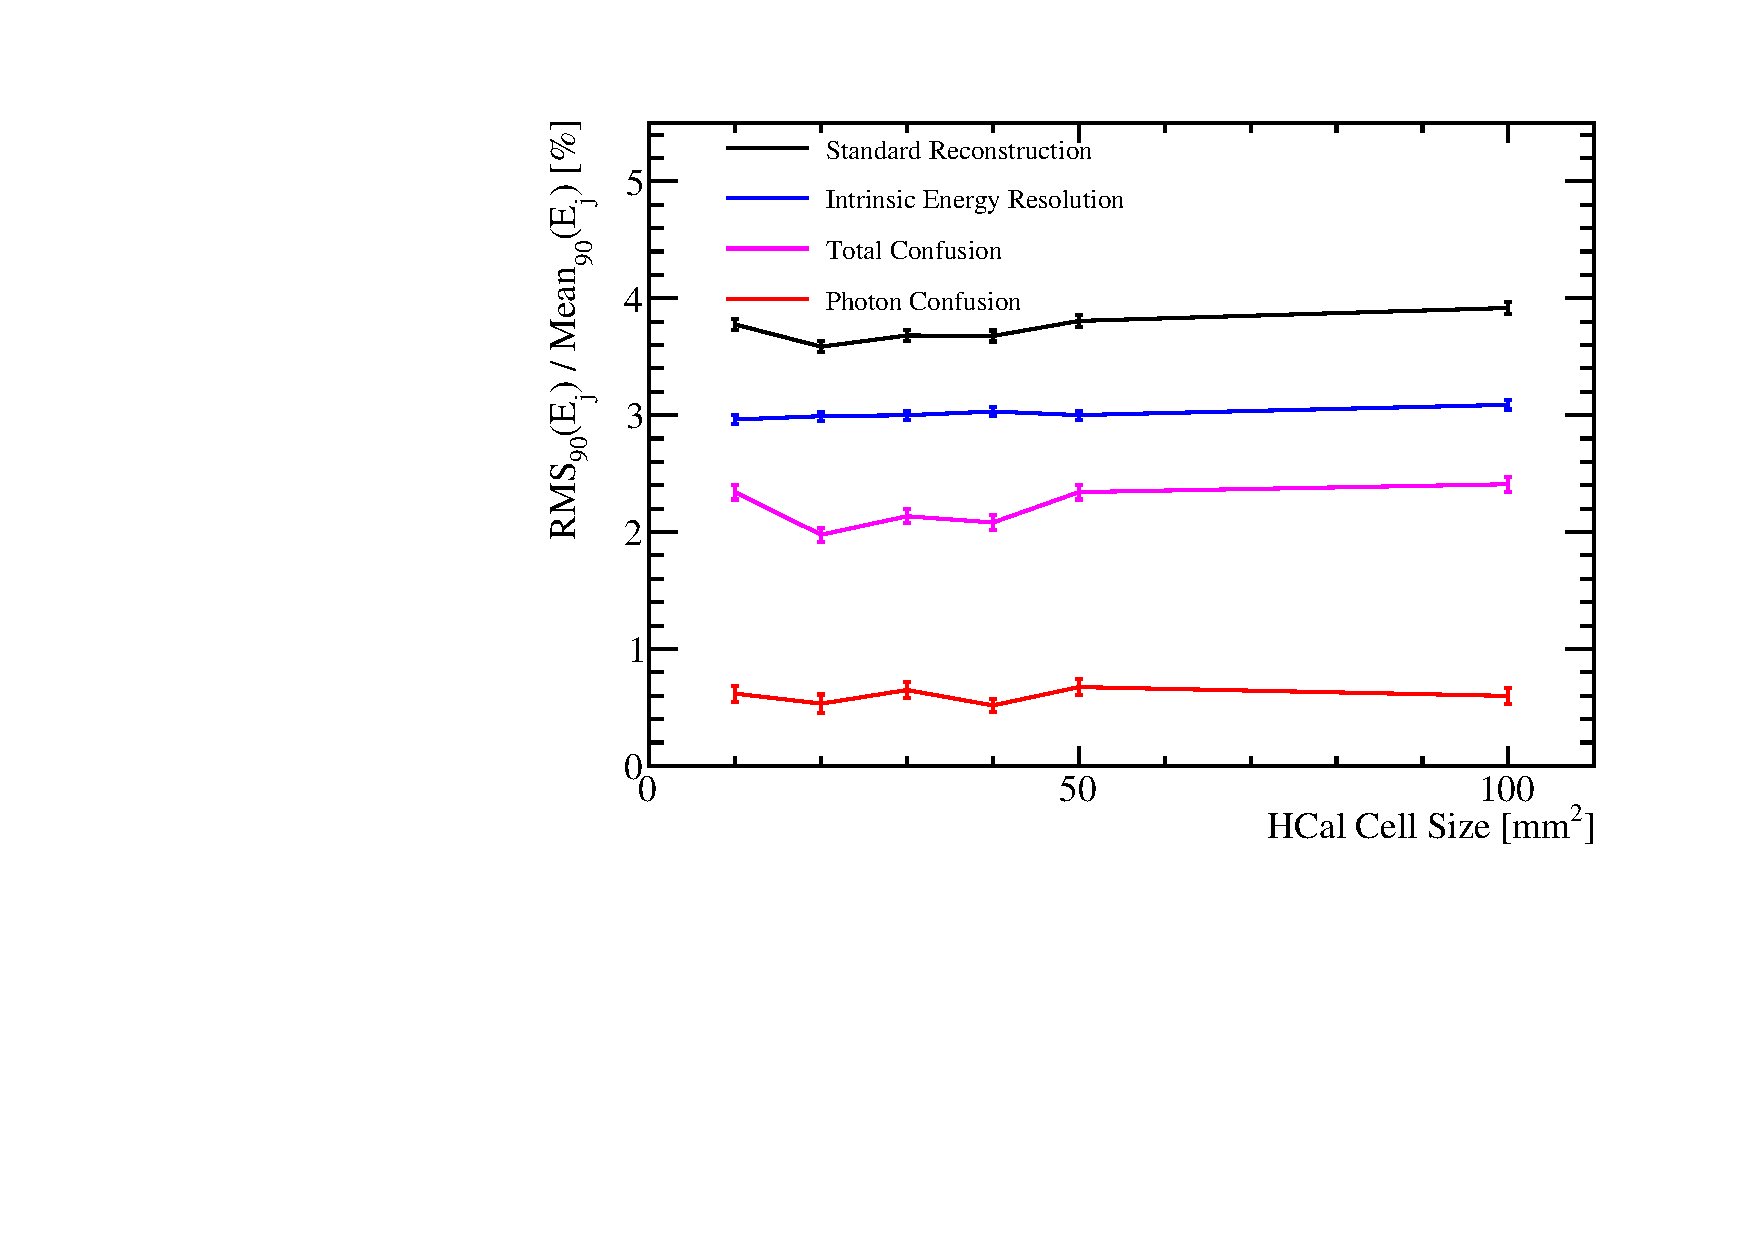
\includegraphics[width=0.5\textwidth]{OptimisationStudies/Plots/JetEnergyResolutions/JER_vs_HCalCellSize_91GeV_DiJet_Breakdown.pdf}}
\subfloat[]{\label{fig:hcalcellsize250break}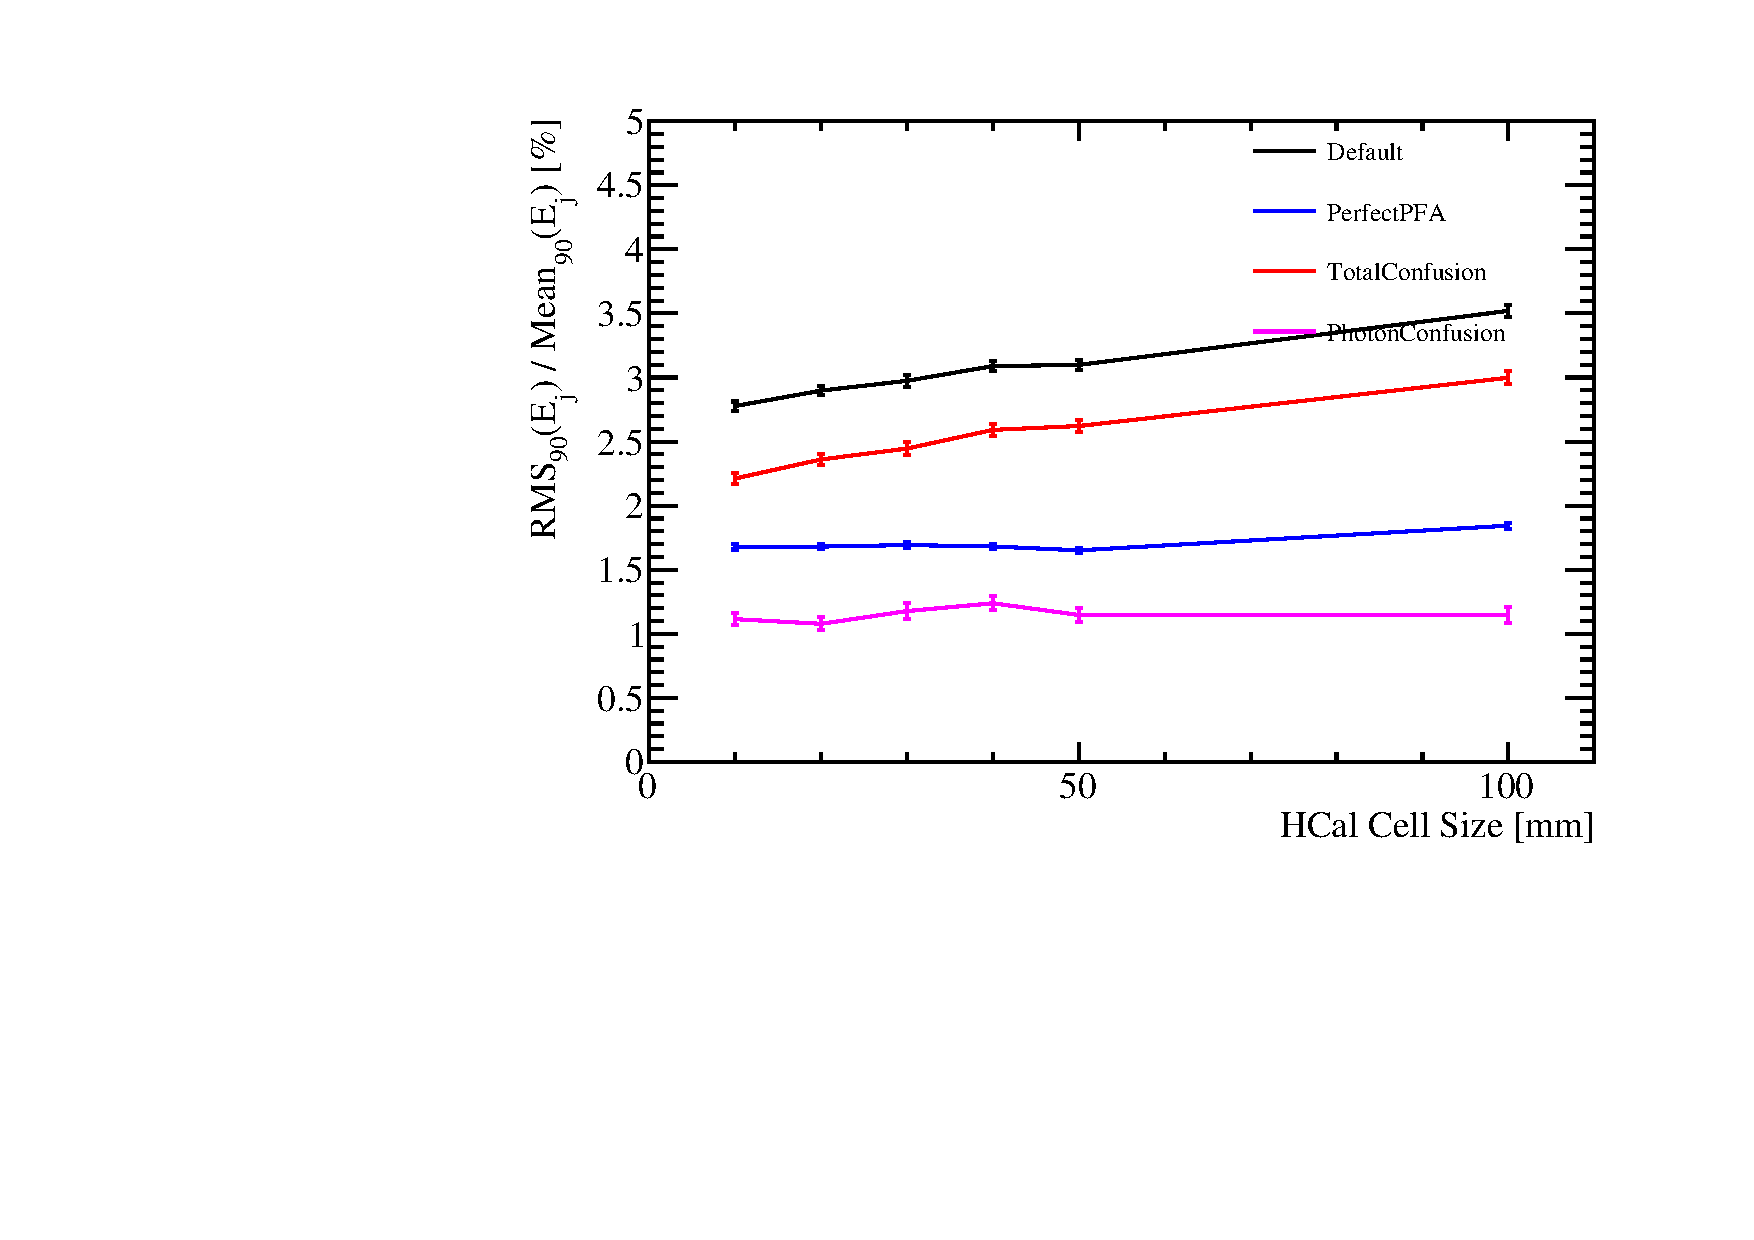
\includegraphics[width=0.5\textwidth]{OptimisationStudies/Plots/JetEnergyResolutions/JER_vs_HCalCellSize_500GeV_DiJet_Breakdown.pdf}}
\caption[The contributions to the jet energy resolution as a function of HCal cell size using the nominal ILD detector model for \protect\subref{fig:hcalcellsize45break} 45 GeV jets and \protect\subref{fig:hcalcellsize250break} 250 GeV jets.  The black curves correspond to the standard reconstruction, the blue curves to the intrinsic energy resolution contribution to the jet energy resolution, the red curves to the confusion contribution to the jet energy resolution and the magenta curves to the confusion contribution to the jet energy resolution related solely to $\gamma$ reconstruction.]{The contributions to the jet energy resolution as a function of HCal cell size using the nominal ILD detector model for \protect\subref{fig:hcalcellsize45break} 45 GeV jets and \protect\subref{fig:hcalcellsize250break} 250 GeV jets.  The black curves correspond to the standard reconstruction, the blue curves to the intrinsic energy resolution contribution to the jet energy resolution, the red curves to the confusion contribution to the jet energy resolution and the magenta curves to the confusion contribution to the jet energy resolution related solely to $\gamma$ reconstruction.}
\label{fig:hcalcellsizebreak}
\end{figure}

The jet energy resolution dependence on the HCal cell size is less strong than that observed in the ECal cell size, but that is to be expected as the ECal cell size determines the position of the start of showering particles in the calorimeters.  If the start of a particle shower is well reconstructed in the ECal it becomes easier to associate the relevant calorimetric energy deposits in the HCal to it and vice verse.  Therefore, a comparison of these studies indicates that ECal cell size is more crucial in the successful application of particle flow calorimetry than the HCal cell size is.

The confusion contribution to the jet energy resolution decreases by reducing the HCal cell size, while the intrinsic energy resolution of the detector is largely invariant to changes in the HCal cell size.  As this dependancy is relatively weak, even the use of 100 mm square HCal cell sizes would be enough to allow for separation of the hadronic decays of W and Z bosons at ILC like energies.  However, as jet energy resolution does improve with decreasing cell sizes it is desirable to have as small a HCal cell size as possible.

%========================================================================================

\subsection{HCal Number of Layers}
\label{sec:hcalnlayers}
The total number of layers in the HCal was varied while leaving the active and absorber layer thicknesses unchanged.  This leads to a change in the total thickness of the calorimeter, but not the sampling frequency of particle showers within it.  It is expected that this study will determine the effects of leakage of energy out of the back of the calorimeter, with a larger number of layers giving a smaller effect from leakage.  The cost of the HCal is proportional to the number of readout channels, which is proportional to the number of layers used in the HCal.  Therefore, minimising the number of layers, while retaining excellent physics performance it vital.  For this study detector models were simulated with a HCal containing 36, 42, 48 (nominal), 54 and 60 layers. 

It is expected that the energy resolution of the detector will improve with an increasing number of layers in the HCal as fewer events will suffer from the effects of leakage in a HCal with more layers.  The improvement is only expected up to a point, as beyond a given point almost all hadronic showers will be fully contained and so additional layers do not impact the energy measurements.  The energy resolution as a function of number of layers in the HCal for 50 GeV $\text{K}^{0}_{L}$ is shown in figure \ref{fig:hcalnfixedlayerser}.  As expected, the energy resolution degrades when the number of layers is reduced below 48 layers, while above this, additional layers do not yield better energy resolutions.  However, even reducing the number of layers to 36 only causes a degradation in the energy resolution of the order of $1\%$.  

\begin{figure}[h!]
\centering
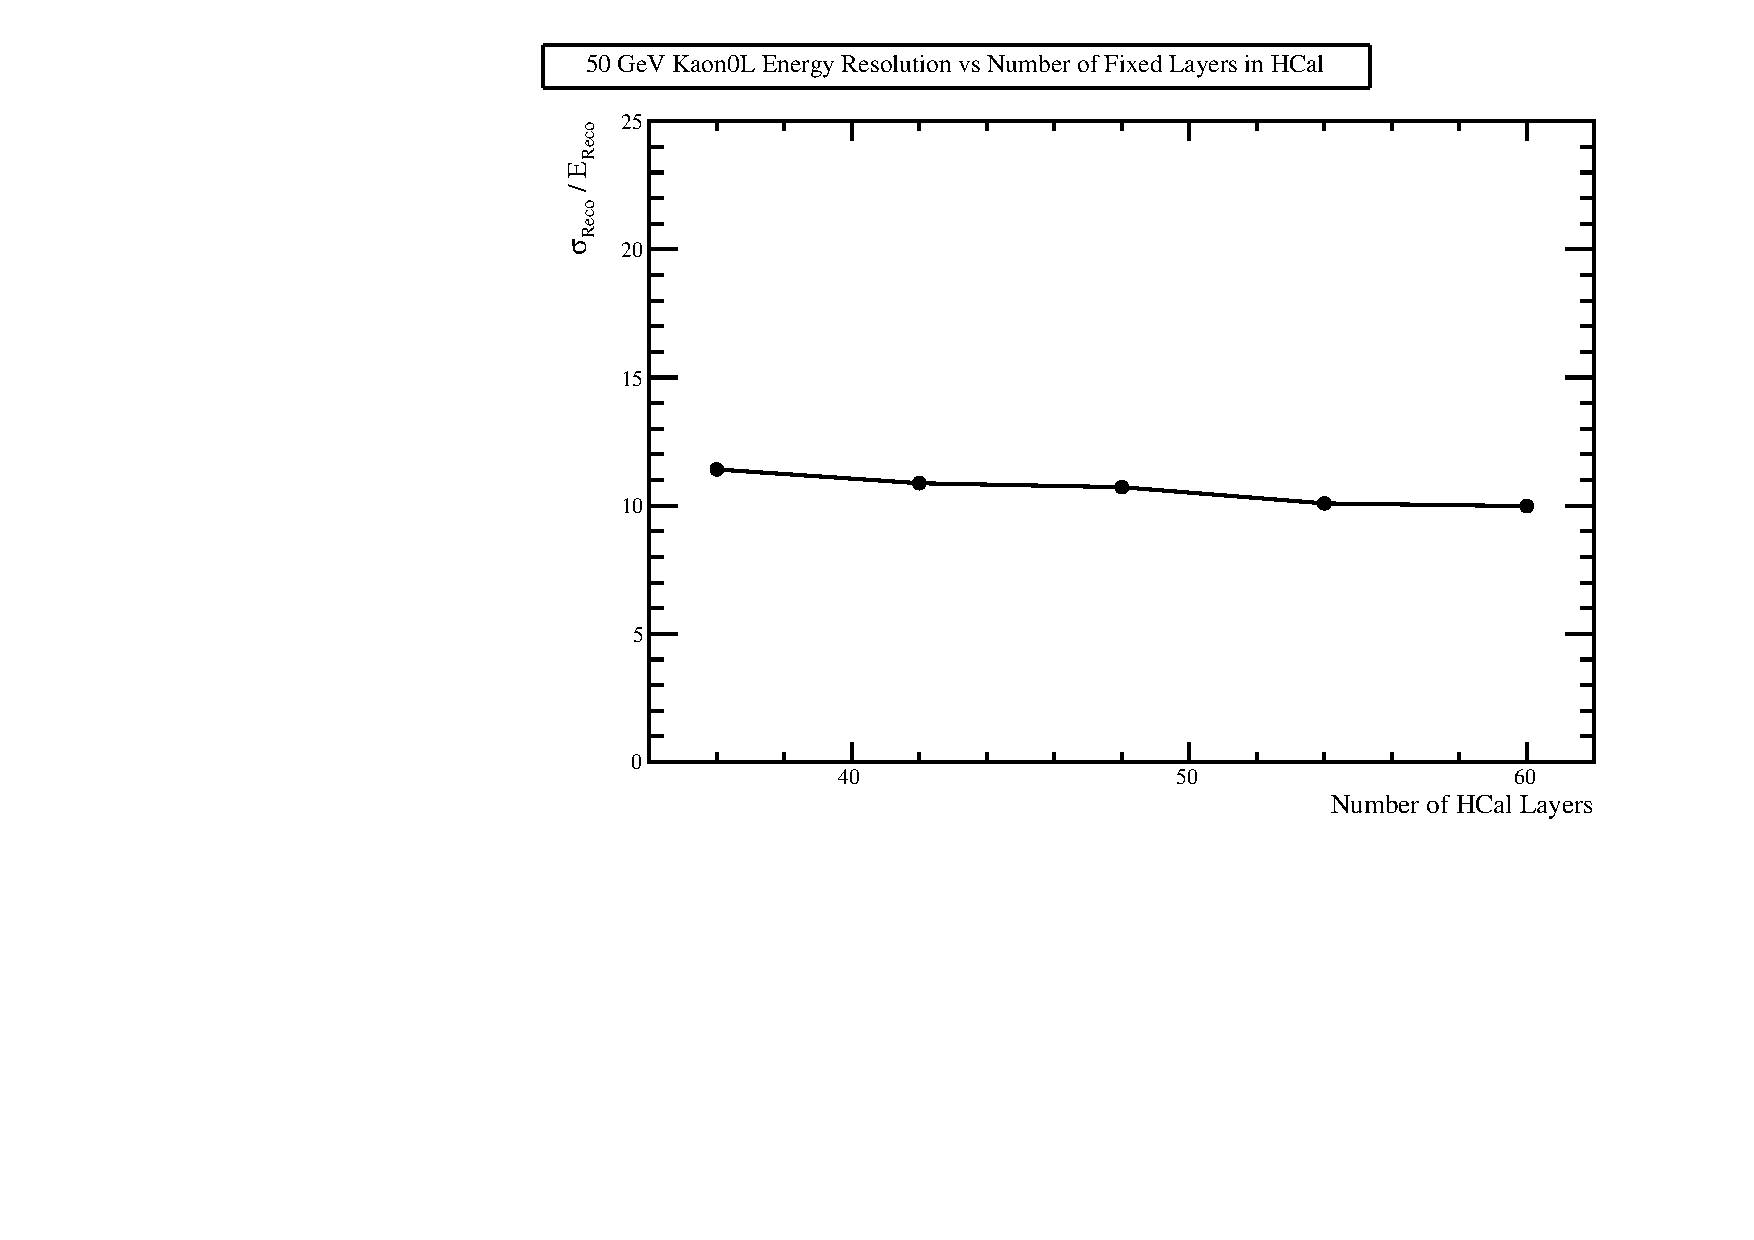
\includegraphics[width=0.5\textwidth]{OptimisationStudies/Plots/EnergyResolution/ER_vs_HCalNFixedLayers_50GeVKaon0L.pdf}
\caption[The energy resolution as a function of number of layers in the HCal for 50 GeV $\text{K}^{0}_{L}$ events using the nominal ILD detector model.]{The energy resolution as a function of number of layers in the HCal for 50 GeV $\text{K}^{0}_{L}$ events using the nominal ILD detector model.}
\label{fig:hcalnfixedlayerser}
\end{figure}

The trend in the 50 GeV $\text{K}^{0}_{L}$ energy resolution when varying the number of layers in the HCal is unlikely to be seen in the jet energy resolution as it is a weak trend and only a small fraction of jet energy is measured within the HCal.  However, the confusion contribution to the jet energy resolution is expected to change as, during the charged particle track to calorimeter cell cluster association, errors will be introduced if energy has leaked from the back of the calorimeter.  For example, if a particle shower from a charged particle suffers heavily from leakage there will be a large disparity between the track momentum and the energy it deposits within the calorimeter.  In that case, PandoraPFA will be overly aggressive in associating other calorimeter energy deposits to this track to account for the energy that has leaked out of the calorimeter, which will introduce errors.  The jet energy resolution as a function of the number of layers in the HCal is shown in figure \ref{fig:hcalnfixedlayers}.  As expected for low energy jets, where intrinsic energy resolution dominates, the jet energy resolution is invariant to the number of layers, while for high jet energies, where confusion dominates, a larger number of layers benefits the jet energy resolution.  When examining the different contributions to the jet energy resolution, shown in figure \ref{fig:hcalnfixedlayersbreak}, it becomes clear that the confusion contribution that drives the observed trends.  On the other hand, the intrinsic energy resolution is largely invariant to changes to the number of HCal layers as only a small fraction of jet energy is recorded in the HCal.  Furthermore, the photon confusion is invariant to changes in the number of HCal layers, indicating that the change in the confusion contribution are originating from pattern recognition involving hadrons.

\begin{figure}[h!]
\centering
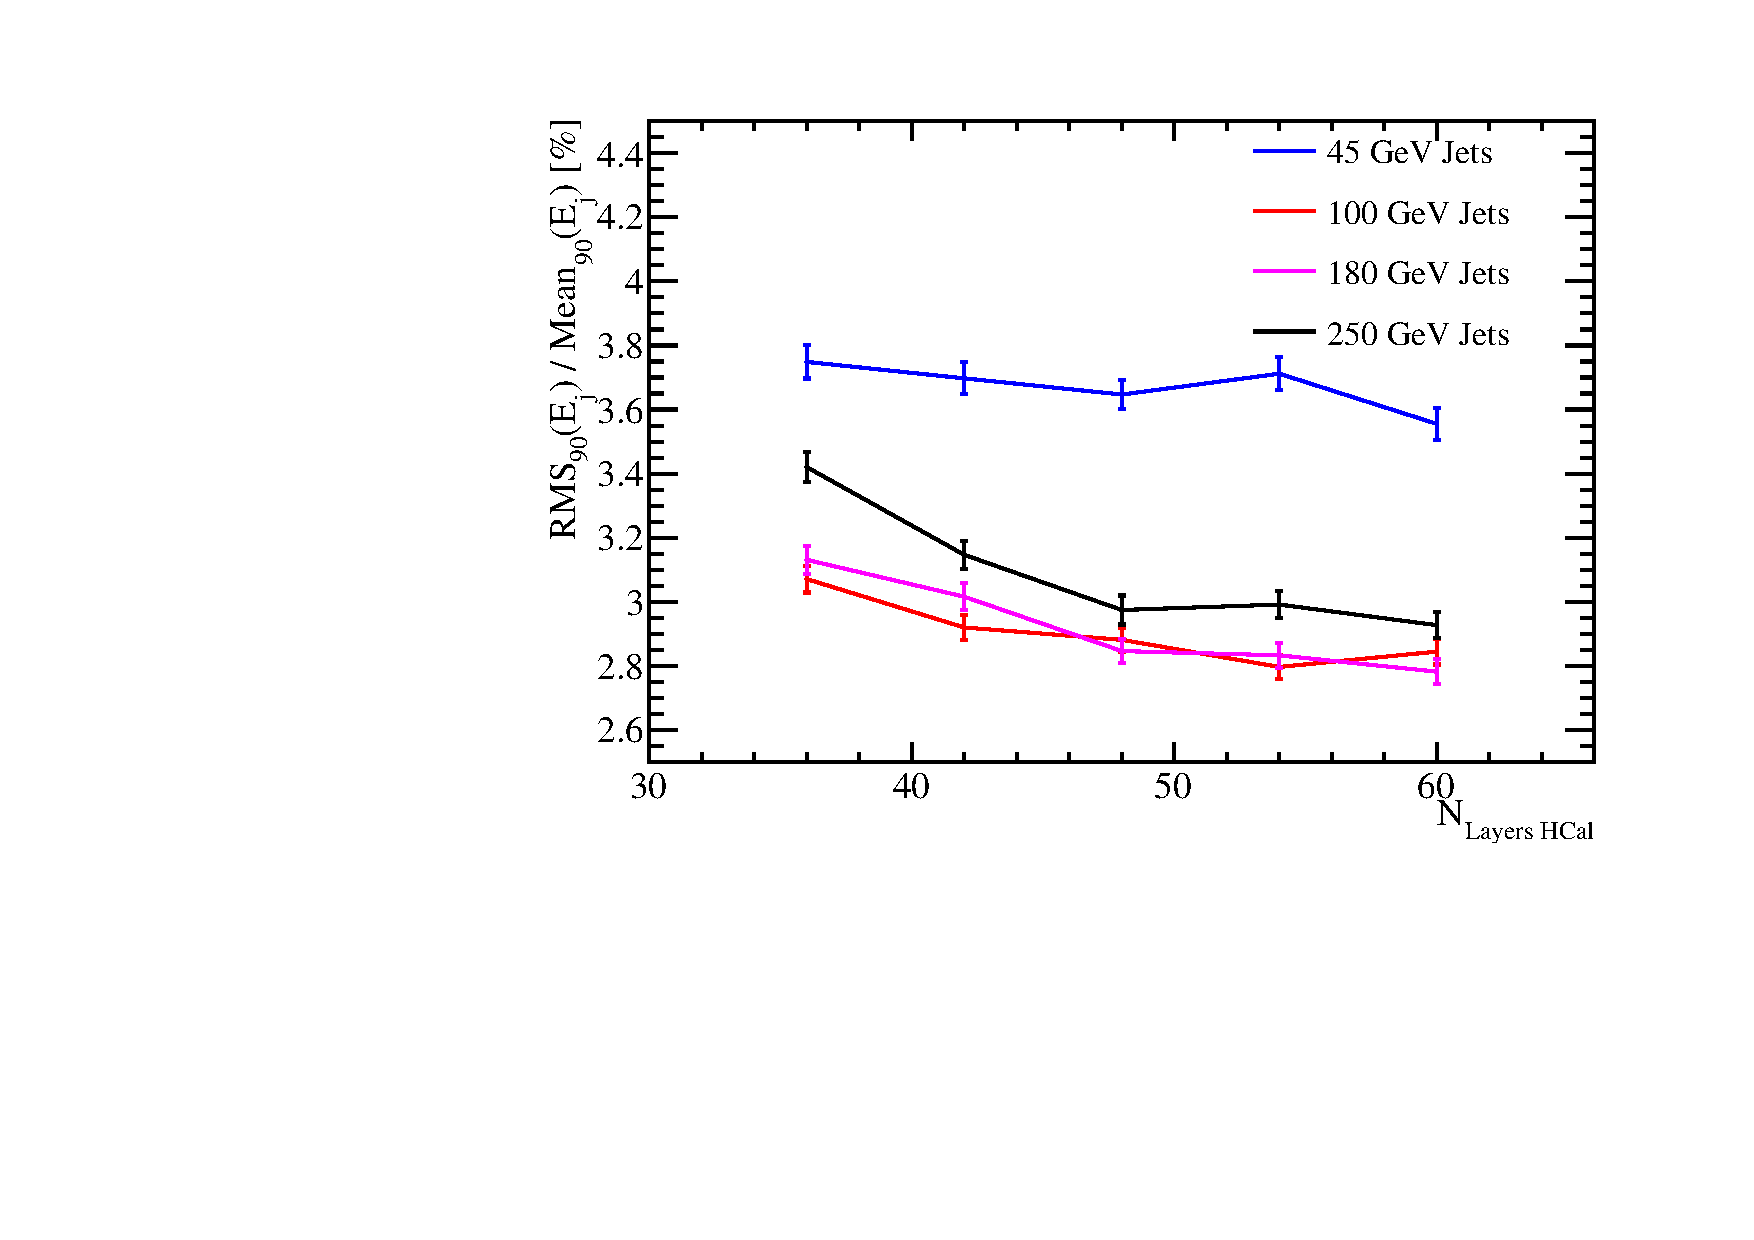
\includegraphics[width=0.5\textwidth]{OptimisationStudies/Plots/JetEnergyResolutions/JER_vs_NumberOfHCalLayersOfFixedDepth.pdf}
\caption[The jet energy resolution as a function of number of layers in the HCal for various jet energies using the nominal ILD detector model.]{The jet energy resolution as a function of number of layers in the HCal for various jet energies using the nominal ILD detector model.}
\label{fig:hcalnfixedlayers}
\end{figure}

\begin{figure}[h!]
\centering
\subfloat[]{\label{fig:hcalnfixedlayers45break}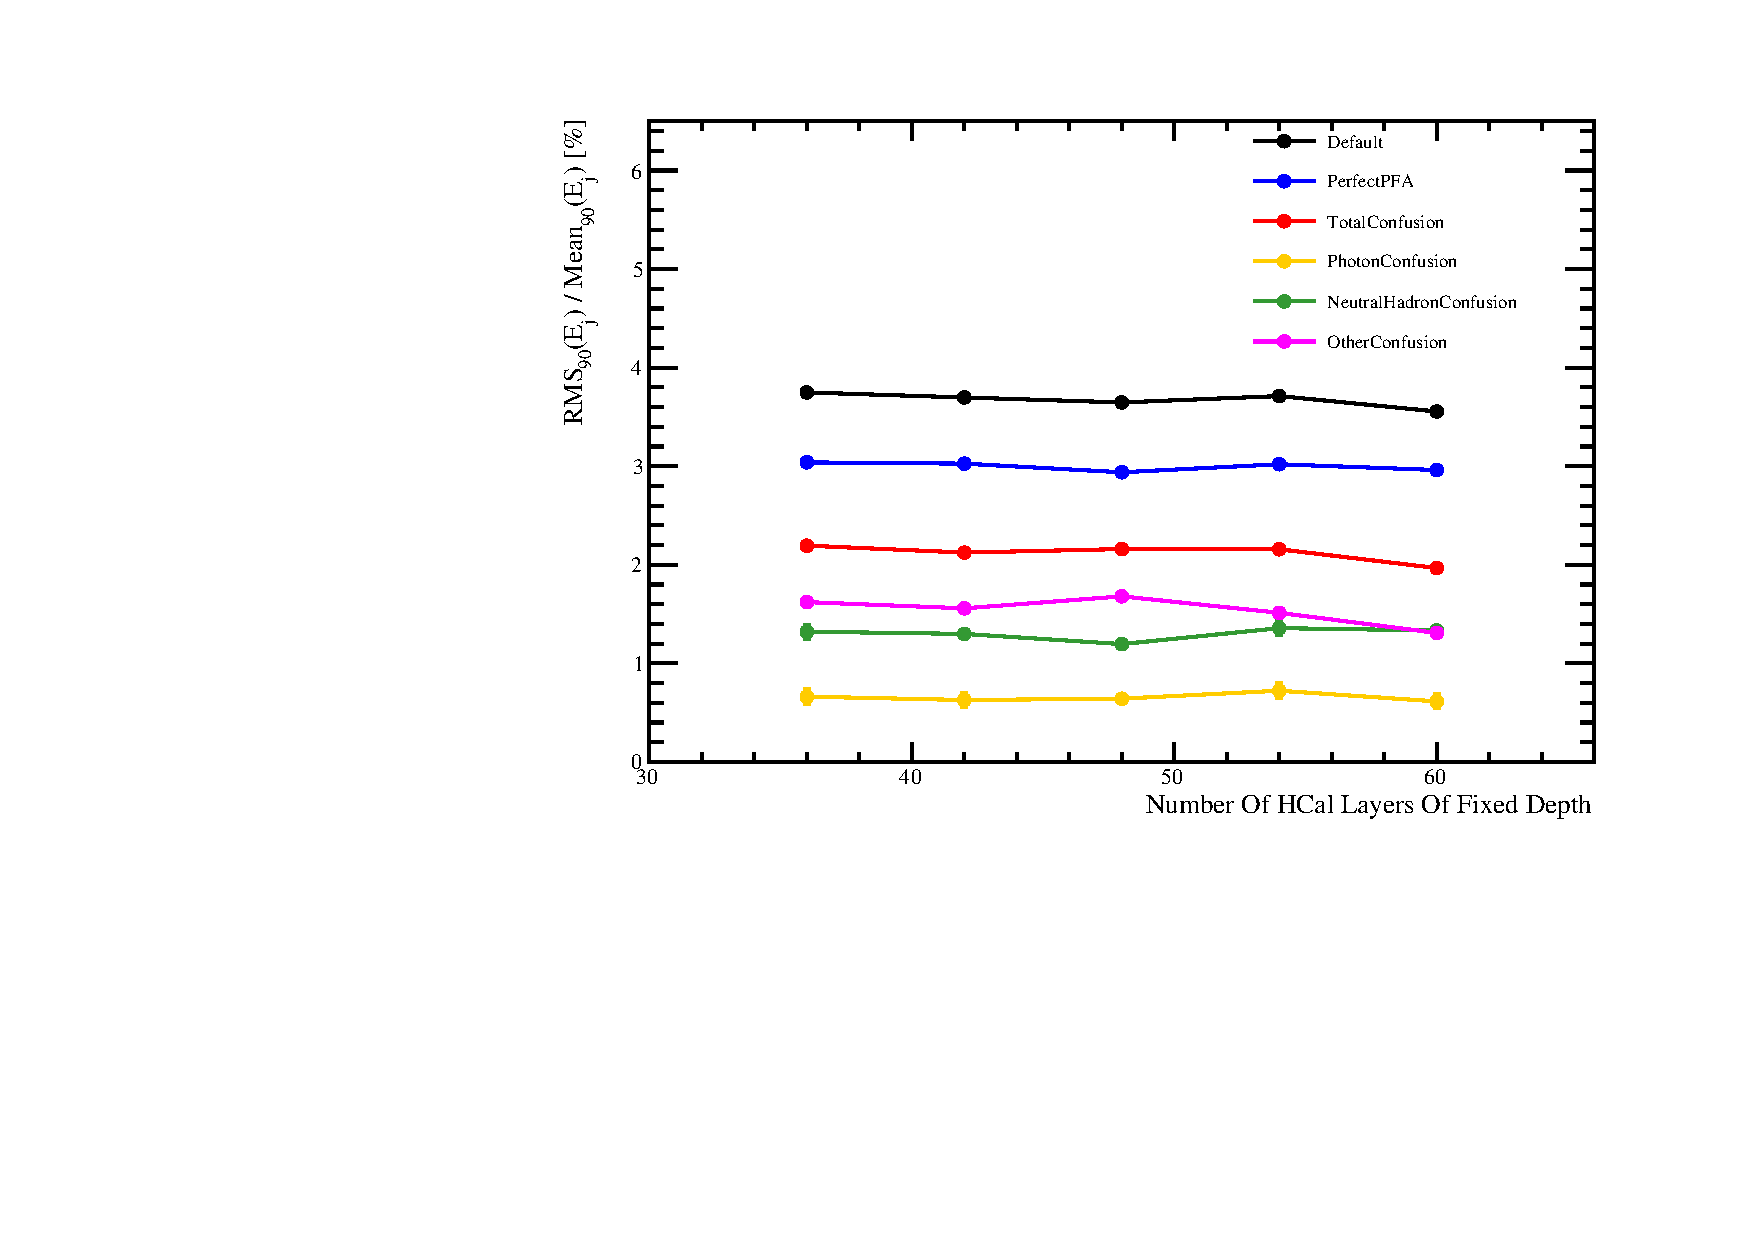
\includegraphics[width=0.5\textwidth]{OptimisationStudies/Plots/JetEnergyResolutions/JER_vs_NumberOfHCalLayersOfFixedDepth_91GeV_DiJet_Breakdown.pdf}}
\subfloat[]{\label{fig:hcalnfixedlayers250break}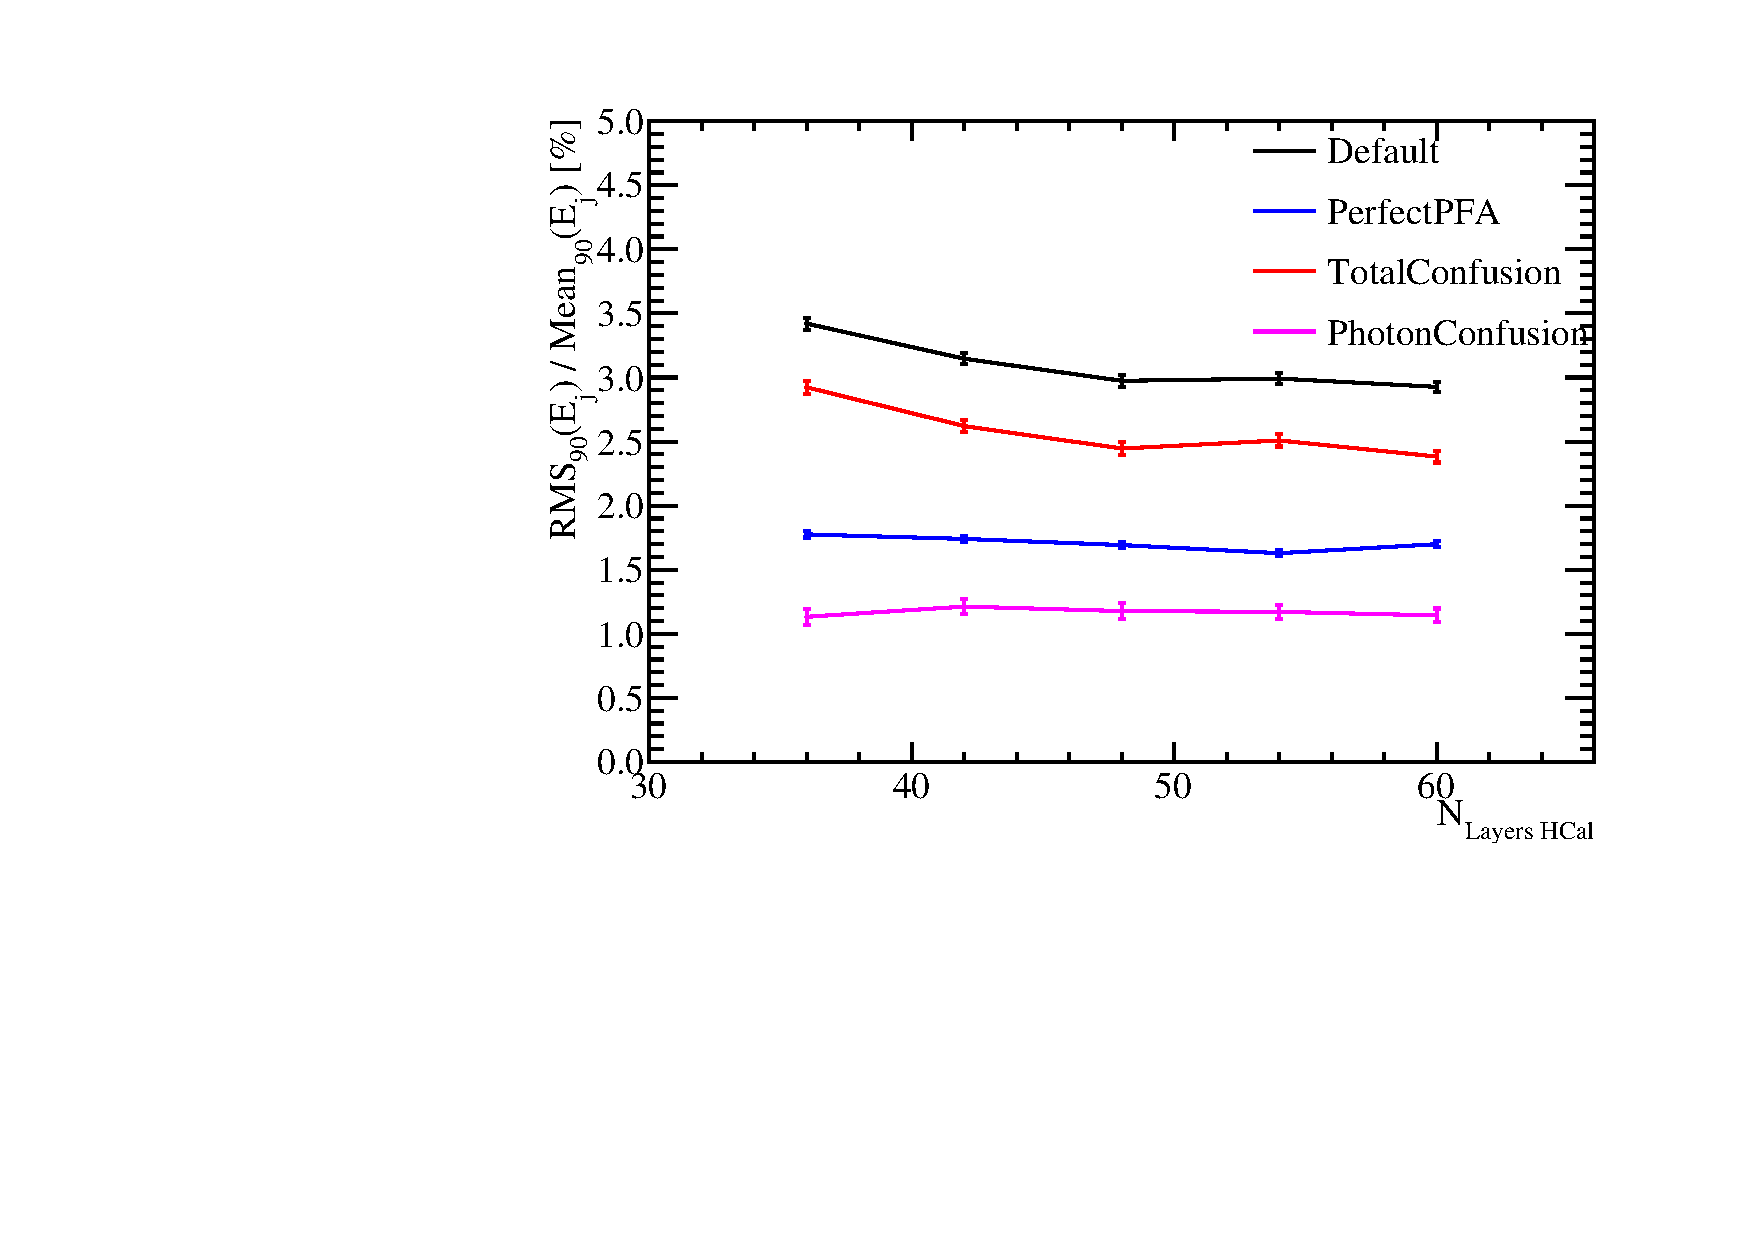
\includegraphics[width=0.5\textwidth]{OptimisationStudies/Plots/JetEnergyResolutions/JER_vs_NumberOfHCalLayersOfFixedDepth_500GeV_DiJet_Breakdown.pdf}}
\caption[The contributions to the jet energy resolution as a function of number of layers in the HCal using the nominal ILD detector model for \protect\subref{fig:hcalnfixedlayers45break} 45 GeV jets and \protect\subref{fig:hcalnfixedlayers250break} 250 GeV jets.  The black curves correspond to the standard reconstruction, the blue curves to the intrinsic energy resolution contribution to the jet energy resolution, the red curves to the confusion contribution to the jet energy resolution and the magenta curves to the confusion contribution to the jet energy resolution related solely to $\gamma$ reconstruction.]{The contributions to the jet energy resolution as a function of number of layers in the HCal using the nominal ILD detector model for \protect\subref{fig:hcalnfixedlayers45break} 45 GeV jets and \protect\subref{fig:hcalnfixedlayers250break} 250 GeV jets.  The black curves correspond to the standard reconstruction, the blue curves to the intrinsic energy resolution contribution to the jet energy resolution, the red curves to the confusion contribution to the jet energy resolution and the magenta curves to the confusion contribution to the jet energy resolution related solely to $\gamma$ reconstruction.}
\label{fig:hcalnfixedlayersbreak}
\end{figure}

In summary, even if the number of layers in the HCal were reduced by a factor of 25\% the jet energy resolution would be sufficient for separating the hadronic decays of the W and Z bosons at ILC energies.  However, it is clear that leakage of energy from the back of the HCal would negatively affect events at ILC like energies should the number of layers be reduced from the nominal value of 48 layers, therefore it is desirable to have a minimum of 48 layers in the HCal.
  
%========================================================================================

\subsection{HCal Sampling Frequency}
\label{sec:hcalsamplingfrequency}
The sampling frequency in the HCal was by varying the number of readout layers in the HCal, while simultaneously varying the active and absorber layer thicknesses such that the total number of nuclear interaction lengths in the HCal is constant.  For each model considered, the absorber material was steel, containing a total of 5.72 $\lambda_{I}$, while the active material was scintillator, containing a total of 0.19 $\lambda_{I}$.  Furthermore, the ratio of the active to absorber layers thicknesses (the sampling fraction) was not changed.  A summary of the detector models considered in this study can be found in table \ref{table:nlayershcaloption}.  

\begin{table}[h!]
\centering
\begin{tabular}{ l l l }
\hline
Number $N_{\text{Layers HCal}}$& Absorber Thickness & Active Thickness \\
 & [mm] & [mm] \\
\hline
60 & 16.00 & 2.40 \\ 
54 & 17.78 & 2.67 \\
48 & 20.00 & 3.00 \\
42 & 22.86 & 3.43 \\
36 & 26.67 & 4.00 \\
30 & 32.00 & 4.80 \\
24 & 40.00 & 6.00 \\
18 & 53.33 & 8.00 \\
\hline
\end{tabular}
\caption[Cell size layout of various HCal models considered.]{Cell size layout of various HCal models considered.}
\label{table:nlayershcaloption}
\end{table}

Increasing the number of layers in the HCal will increase the number of times a showering particle is sampled, which in turn will reduce the stochastic term in the energy resolution for a sampling calorimeter.  Therefore, it is expected that the energy resolution will improve with increasing number of layers in the HCal.  This is shown for 50 GeV $\text{K}^{0}_{L}$ in figure \ref{fig:hcalnlayerser}.  Although there are fluctuations in the energy resolution, due to both fitting the Gaussian to extract the energy resolution and in the calibration of the detector, there is a clear trend showing that the energy resolution of the calorimeter is strongly dependent upon the sampling frequency in the HCal.   The trend in the energy resolution does not exactly follow a $\frac{1}{\sqrt{N_{\text{Readout Layers HCal}}}}$ relationship, but this is to be expected as this relationship only holds for the energy resolution of the HCal.  On the other hand, these results are for the whole ILD detector, including the $\approx 1 \lambda_{I}$ in the ECal.  Furthermore, this functional form neglects the constant term in the energy resolution described in section \ref{sec:nominaldetectorperformance}.  

\begin{figure}[h!]
\centering
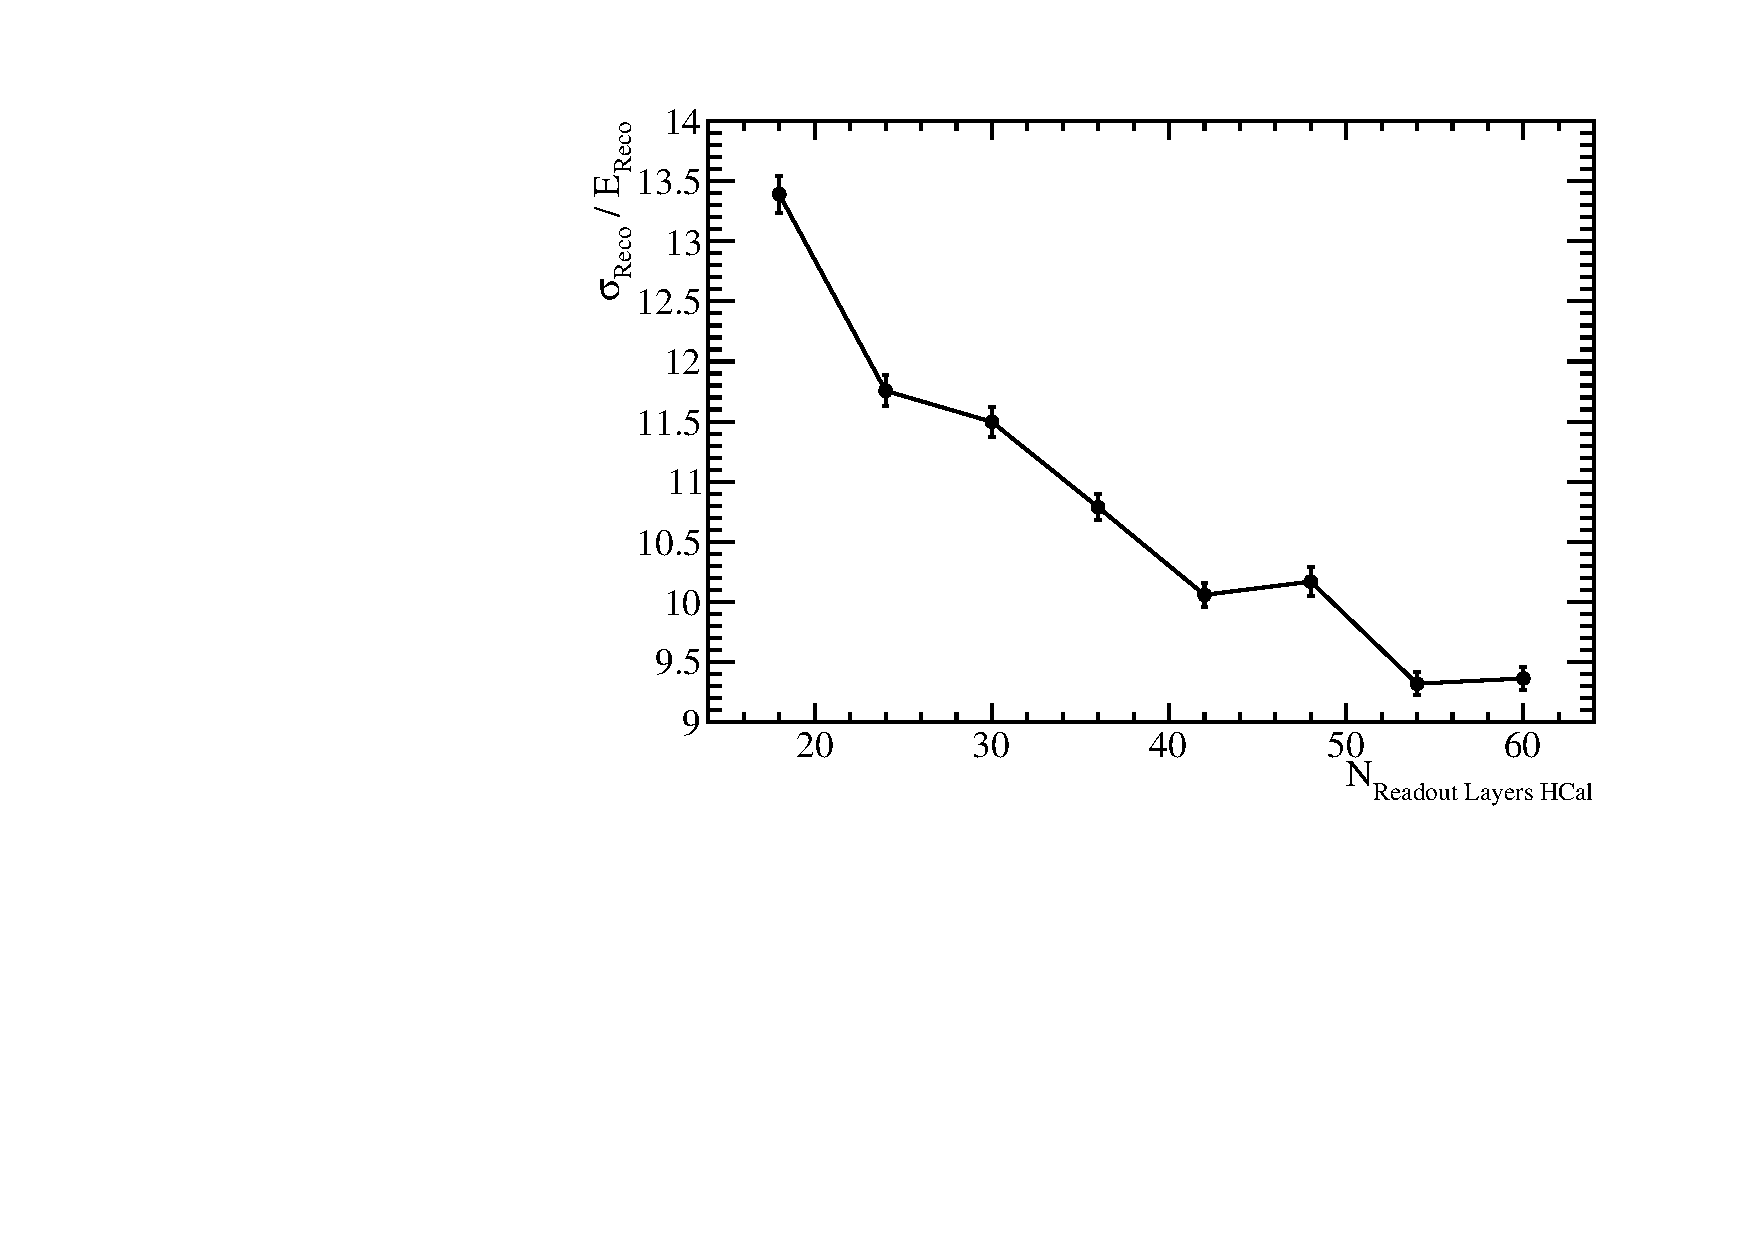
\includegraphics[width=0.5\textwidth]{OptimisationStudies/Plots/EnergyResolution/ER_vs_NHCalVariableLayers_50GeVKaon0L.pdf}
\caption[The energy resolution as a function of sampling frequency in the HCal for 50 GeV $\text{K}^{0}_{L}$ events using the nominal ILD detector model.]{The energy resolution as a function of sampling frequency in the HCal for 50 GeV $\text{K}^{0}_{L}$ events using the nominal ILD detector model.}
\label{fig:hcalnlayerser}
\end{figure}

As changing the sampling frequency of a calorimeter alters the intrinsic energy resolution, it is expected that this will produce a twofold effect on the jet energy resolution whereby the intrinsic energy improvements have the knock on effect of lowering confusion, as described in section \ref{sec:ecalnlayers}, for changes to the number of layers in the ECal.  The jet energy resolution as a function of sampling frequency in the HCal is shown in figure \ref{ig:hcalnlayers}.  As expected there is an improvement in jet energy resolution at all energies due as both the intrinsic energy resolution and confusion are reduced with increasing sampling frequency, which can be seen when examining the different contributions to the jet energy resolution, shown in figure \ref{fig:hcalnlayersbreak}.  

\begin{figure}[h!]
\centering
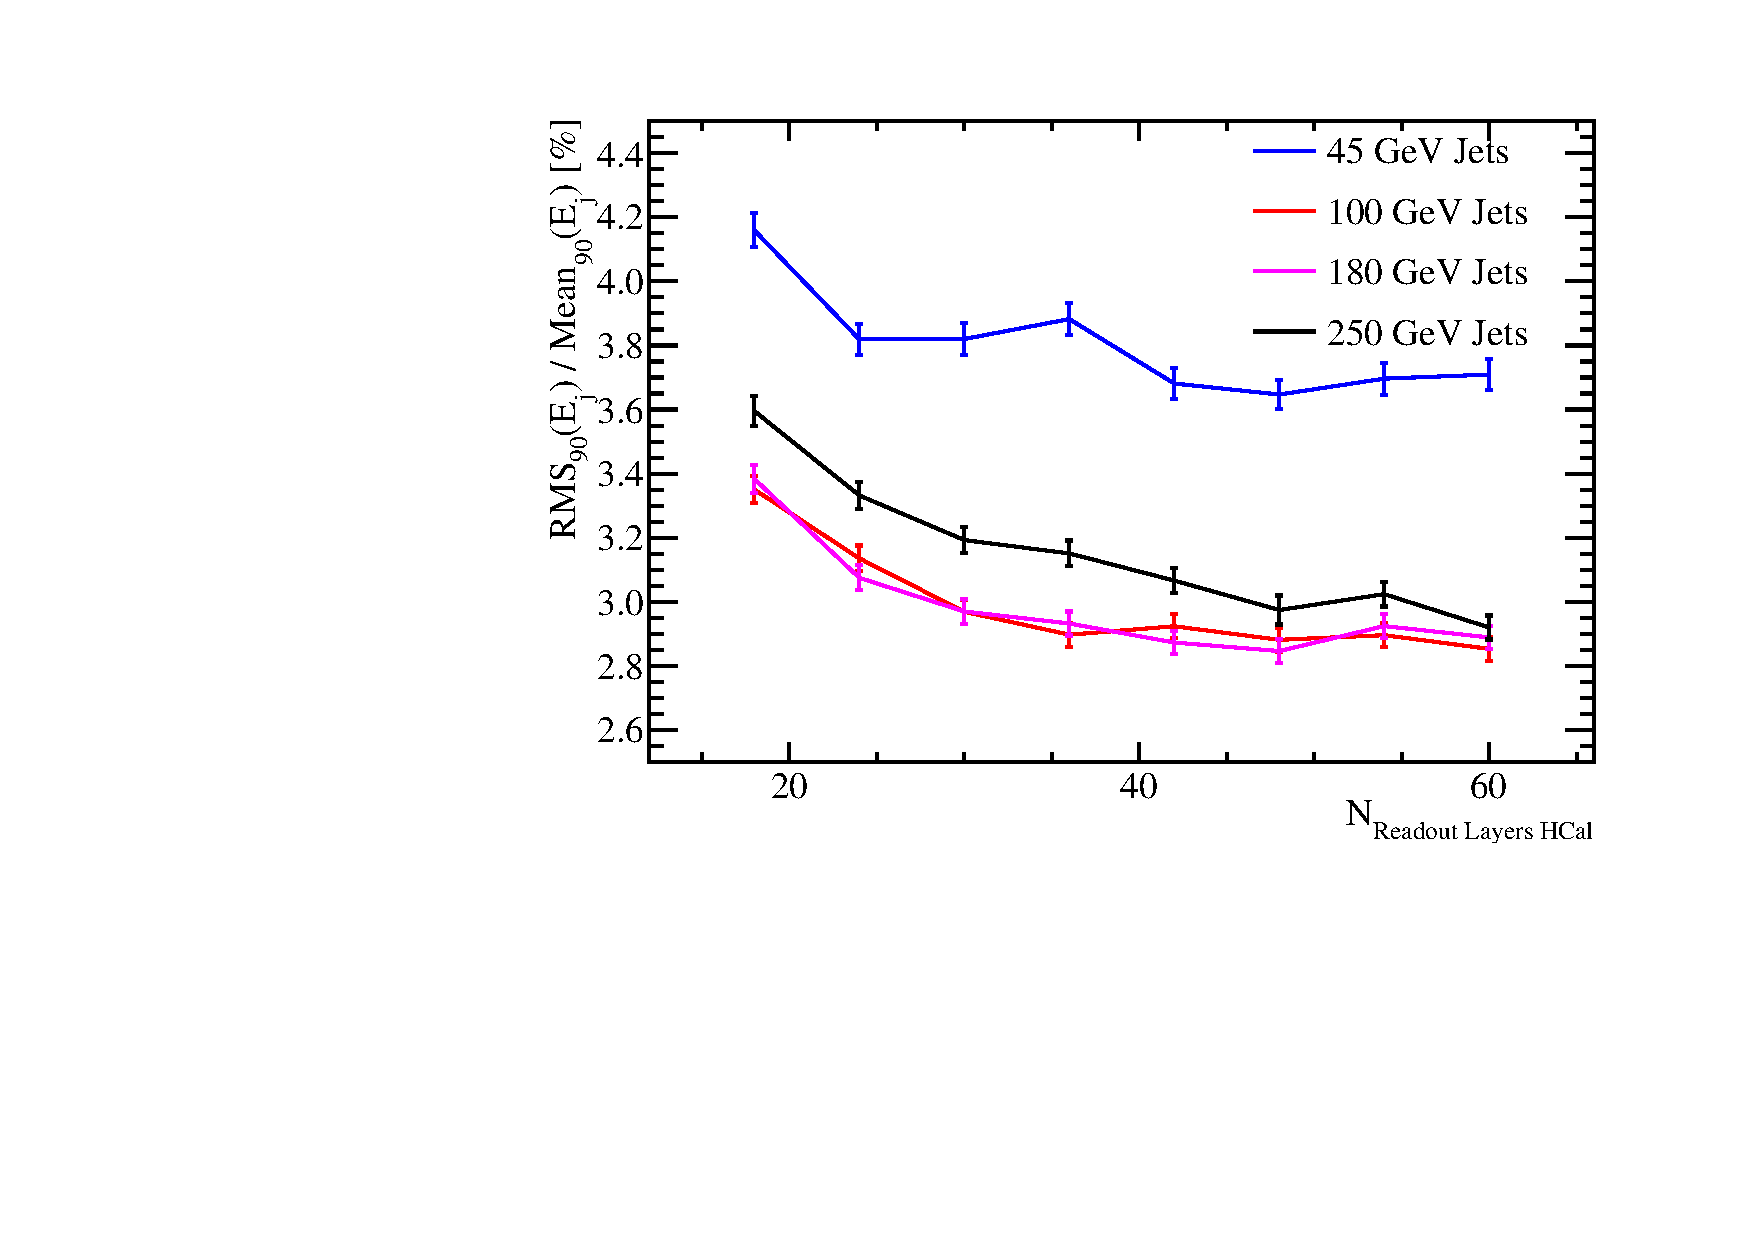
\includegraphics[width=0.5\textwidth]{OptimisationStudies/Plots/JetEnergyResolutions/JER_vs_NumberOfLayersInTheHCal.pdf}
\caption[The jet energy resolution as a function of sampling frequency in the HCal for various jet energies using the nominal ILD detector model.]{The jet energy resolution as a function of sampling frequency in the HCal for various jet energies using the nominal ILD detector model.}
\label{fig:hcalnlayers}
\end{figure}

\begin{figure}[h!]
\centering
\subfloat[]{\label{fig:hcalnlayers45break}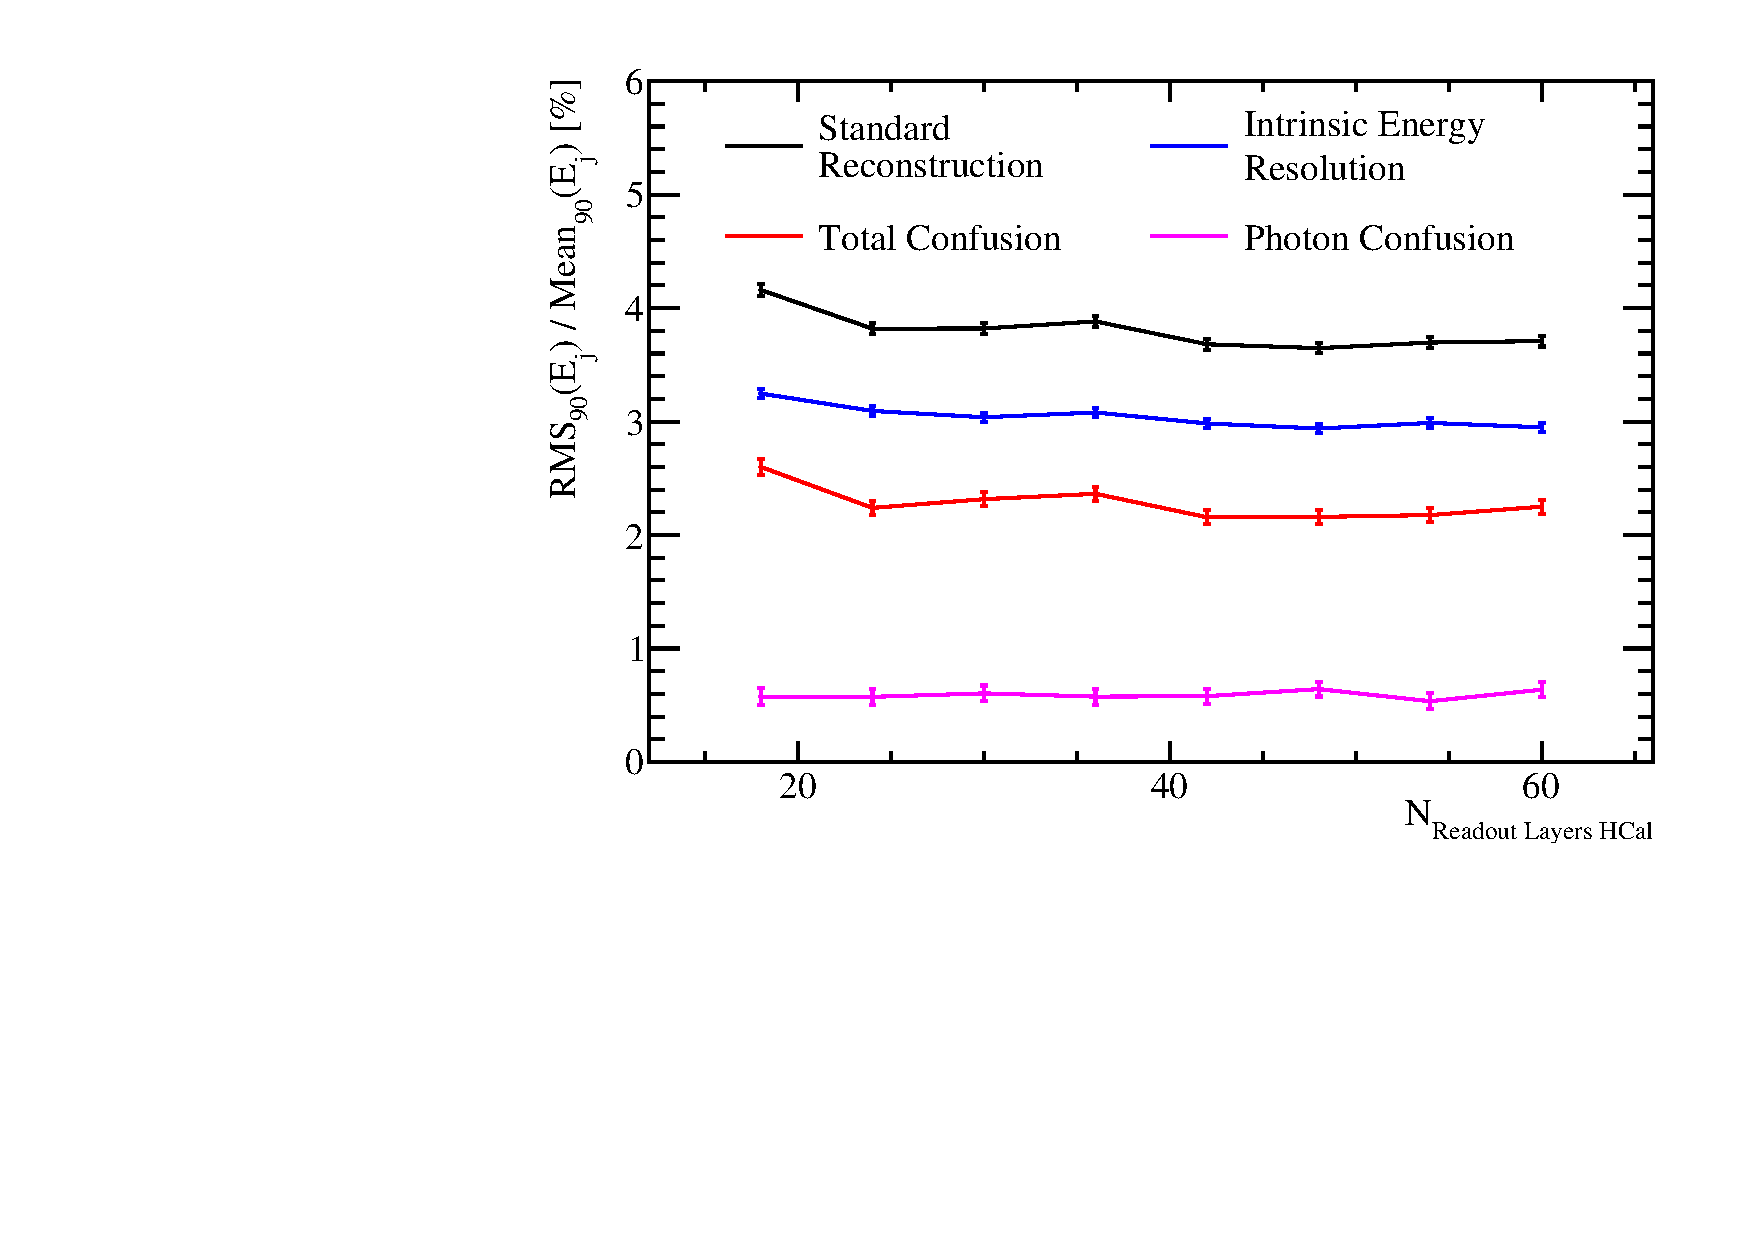
\includegraphics[width=0.5\textwidth]{OptimisationStudies/Plots/JetEnergyResolutions/JER_vs_NumberOfLayersInTheHCal_91GeV_DiJet_Breakdown.pdf}}
\subfloat[]{\label{fig:hcalnlayers250break}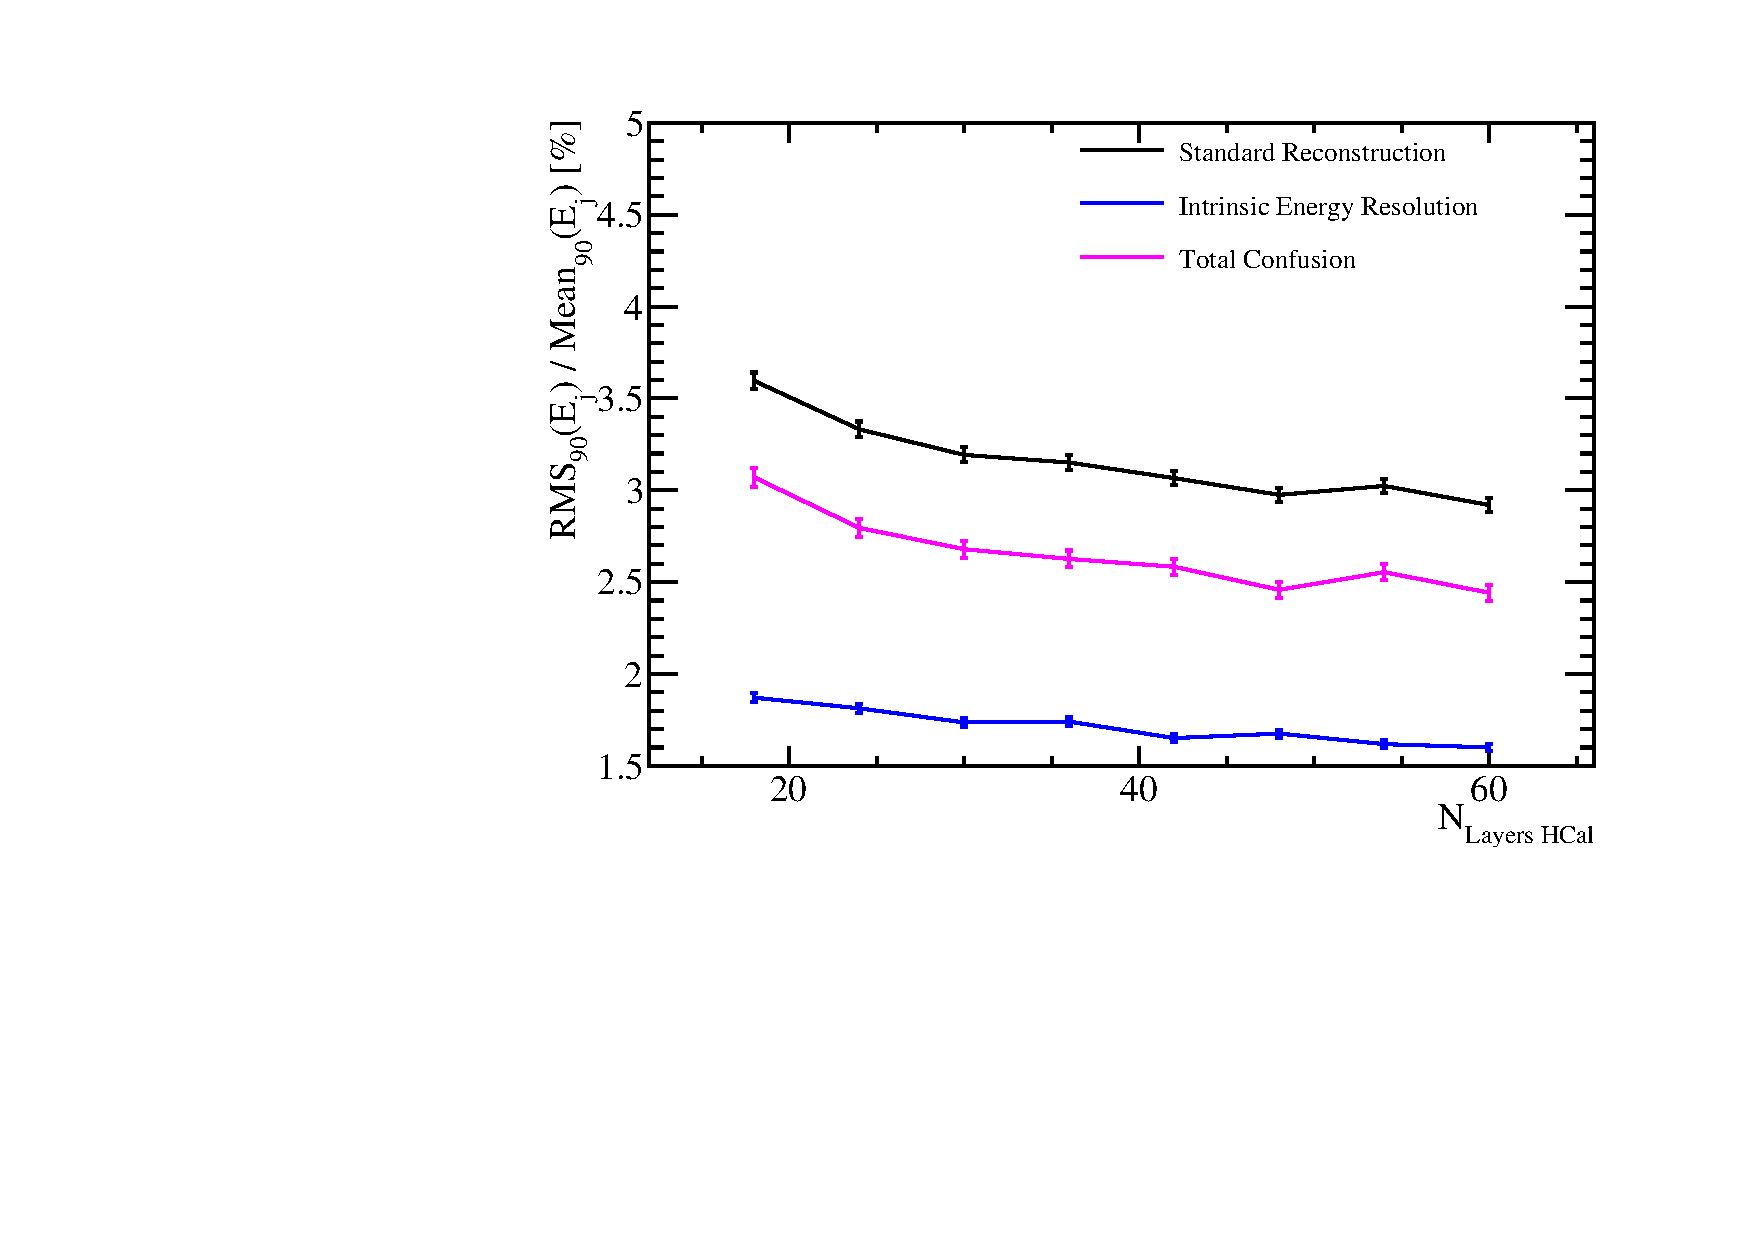
\includegraphics[width=0.5\textwidth]{OptimisationStudies/Plots/JetEnergyResolutions/JER_vs_NumberOfLayersInTheHCal_500GeV_DiJet_Breakdown.pdf}}
\caption[The contributions to the jet energy resolution as a function of sampling frequency in the HCal using the nominal ILD detector model for \protect\subref{fig:hcalnlayers45break} 45 GeV jets and \protect\subref{fig:hcalnlayers250break} 250 GeV jets.  The black curves correspond to the standard reconstruction, the blue curves to the intrinsic energy resolution contribution to the jet energy resolution, the red curves to the confusion contribution to the jet energy resolution and the magenta curves to the confusion contribution to the jet energy resolution related solely to $\gamma$ reconstruction.]{The contributions to the jet energy resolution as a function of sampling frequency in the HCal using the nominal ILD detector model for \protect\subref{fig:hcalnlayers45break} 45 GeV jets and \protect\subref{fig:hcalnlayers250break} 250 GeV jets.  The black curves correspond to the standard reconstruction, the blue curves to the intrinsic energy resolution contribution to the jet energy resolution, the red curves to the confusion contribution to the jet energy resolution and the magenta curves to the confusion contribution to the jet energy resolution related solely to $\gamma$ reconstruction.}
\label{fig:hcalnlayersbreak}
\end{figure}

It is clear that a larger number of layers in the HCal benefits both the intrinsic energy resolution of the ILD detector as well as reducing the confusion contribution to the jet energy resolution.  As there are few physics analyses that rely on the identification and categorisation of individual neutral hadrons, but there are many that rely on identification and categorisation of $\gamma$s, the intrinsic energy resolution of the HCal is less crucial from a physics perspective than that of the ECal.  However, these studies show the HCal still has a crucial role to play in jet reconstruction in the particle flow paradigm and therefore cannot be neglected.  To achieve a jet energy resolution of $\frac{\sigma_{E}}{E} \lesssim 3.8\%$, which is required to separate the W and Z hadronic decays, the ILD detector will require a minimum of 42 layers in the HCal.  This sampling frequency is required in particular for lower energy jets where the energy resolution is dominated by the intrinsic energy resolution of the detector, while at higher energies the resolution is more than good enough to achieve the separation of the decay channels.  

%========================================================================================

\subsection{HCal Sampling Fraction}
\label{sec:hcalsamplingfraction}
The ILD detector performance was simulated where the ratio of the active to absorber layer thicknesses in the HCal were varied.  In the nominal detector model the active scintillator layer thickness is 3 mm, while the absorber layer thickness is 20 mm giving a sampling fraction of 0.15.  HCal models were simulated where this ratio was changed from 0.05 to 0.25 in steps of 0.05, while retaining the same number of interaction lengths in the absorber and active layers as is found in the nominal HCal model.  If the active layer thickness becomes excessively small then it is possible that any signal produced in that layer would be insufficient to accurately estimate the energy deposited within the surrounding absorber layers.  However, no performance differences were observed for any of these detector models when considering the energy resolution for 50 GeV $\text{K}^{0}_{L}$ events or the jet energy resolution for the 91, 200, 360 and 500 GeV Z$\rightarrow$uds di-jet events.  This indicates the particle showers are sufficiently well sampled in all detector models considered and that thinning the active layer of the ILD HCal down to $\sim1$~mm would not harm the detector performance.  

%========================================================================================

\subsection{HCal Absorber Material}
\label{sec:hcalabsorbermaterial}

The nominal choice of absorber material is steel wiht tungsten providing a feasible alternative.  Although tungsten is more expensive than steel, it contains a larger number of nuclear interaction lengths per unit length.  Therefore, using tungsten as opposed to steel as the absorber material would reduce the size of the HCal, while retaining the same number of nuclear interaction lengths.  Reducing the depth of the calorimeter would decrease the size of the solenoid required, which would offset some of the additional cost if tungsten were used as the absorber material. 

\begin{table}[h!]
\centering
\begin{tabular}{ l l l }
\hline
Parameter & Steel HCal Option & Tungsten HCal Option \\
\hline
Cell Size & $30 \times 30 \text{mm}^{2}$ square cells & $30 \times 30 \text{mm}^{2}$ square cells\\
Number of Layers & 48 readout layers & 48 readout layers\\
Absorber Material Thickness [mm] & 20.0 & 12.0 \\
Active Material Choice & Scintillator & Scintillator \\
Active Material Thickness [mm] & 3.0 & 1.8 \\
\hline
\end{tabular}
\caption[The configuration of the stainless steel and tungsten HCal options.]{The configuration of the stainless steel and tungsten HCal options.}
\label{table:hcalabsmaterial}
\end{table}

The configuration for the stainless steel and tungsten HCal options that were used in the full ILD simulation can be found in table \ref{table:hcalabsmaterial}.  To isolate the effects of changing the absorber material, the total depth, in nuclear interaction lengths, was kept constant when comparing these two options.  Furthermore, the sampling fraction was also held constant.  The interaction of hadrons with the absorber material within the detector is simulated by GEANT4.  A number of different physics lists exist within GEANT4 for the modelling of hadronic showers.  The default model for high energy physics calorimetry is the QGSP\_BERT physics list, which uses the quark-gluon string model \cite{Folger:2003sb} with the precompound model of nuclear evaporation \cite{geantStringModel} (QGSP) for high energy interactions and the Bertini (BERT) cascade model \cite{Guthrie:1968ue} for intermediate energy interactions.  For this study both the QGSP\_BERT and the QGSP\_BERT\_HP physics lists were used.  The QGSP\_BERT\_HP list uses the high precision neutron package (NeutronHP) to deal with the transportation of neutrons from below 20 MeV to thermal energies.  This added detail was thought to be necessary for a study involving tungsten due to the expected increase in shower development.    

One of the dominant processes governing the energy deposition of hadronic showers in calorimeters is spallation \cite{Wigmans:2000vf}.  Spallation begins with the collision of a high energy incident particle with an atomic nuclei from the calorimeter absorbing material.  This collision creates an internuclear cascade where a shower of high energy hadronic particles, e.g. protons, neutrons and pions, are produced within the nucleus.  If these energies are large enough, some of these particles may escape the nucleus and form secondary particles in the hadronic shower.  After this initial collision, the nuclei of the absorbing material are left in an excited state.  Assuming the excited nuclei are sufficiently stable that they will not undergo fission, they will return to a stable state by ejecting energy in the form of particles in a process called evaporation.  Evaporation of neutrons, which is the dominant form of evaporation, significantly delays the growth of hadronic showers as some of these neutrons undergo neutron capture \cite{Adloff:2014rya}.  Neutron capture involves an absorber nuclei capturing a neutron and then emitting a $\gamma$ as it returns to a stable state.  Therefore, the time it take for the neutron capture mechanism to proceed is limited by the lifetime of the unstable nuclei.  This makes neutron capture one of the slowest mechanisms by which hadronic showers can propagate.  As absorber materials with a large atomic number, Z, have a larger number of neutrons, it is expected that there will be an increase in the number of evaporation neutrons within hadronic showers developing in such materials.  In turn this will lead to more neutron capture processes and a longer development time for the hadronic showers.  This is what is observed when considering the shower development times using the tungsten (Z=74) and steel (iron, Z=26) HCal options as seen in figure \ref{fig:hcalabsmaterialtiming}. 

\begin{figure}[h!]
\centering
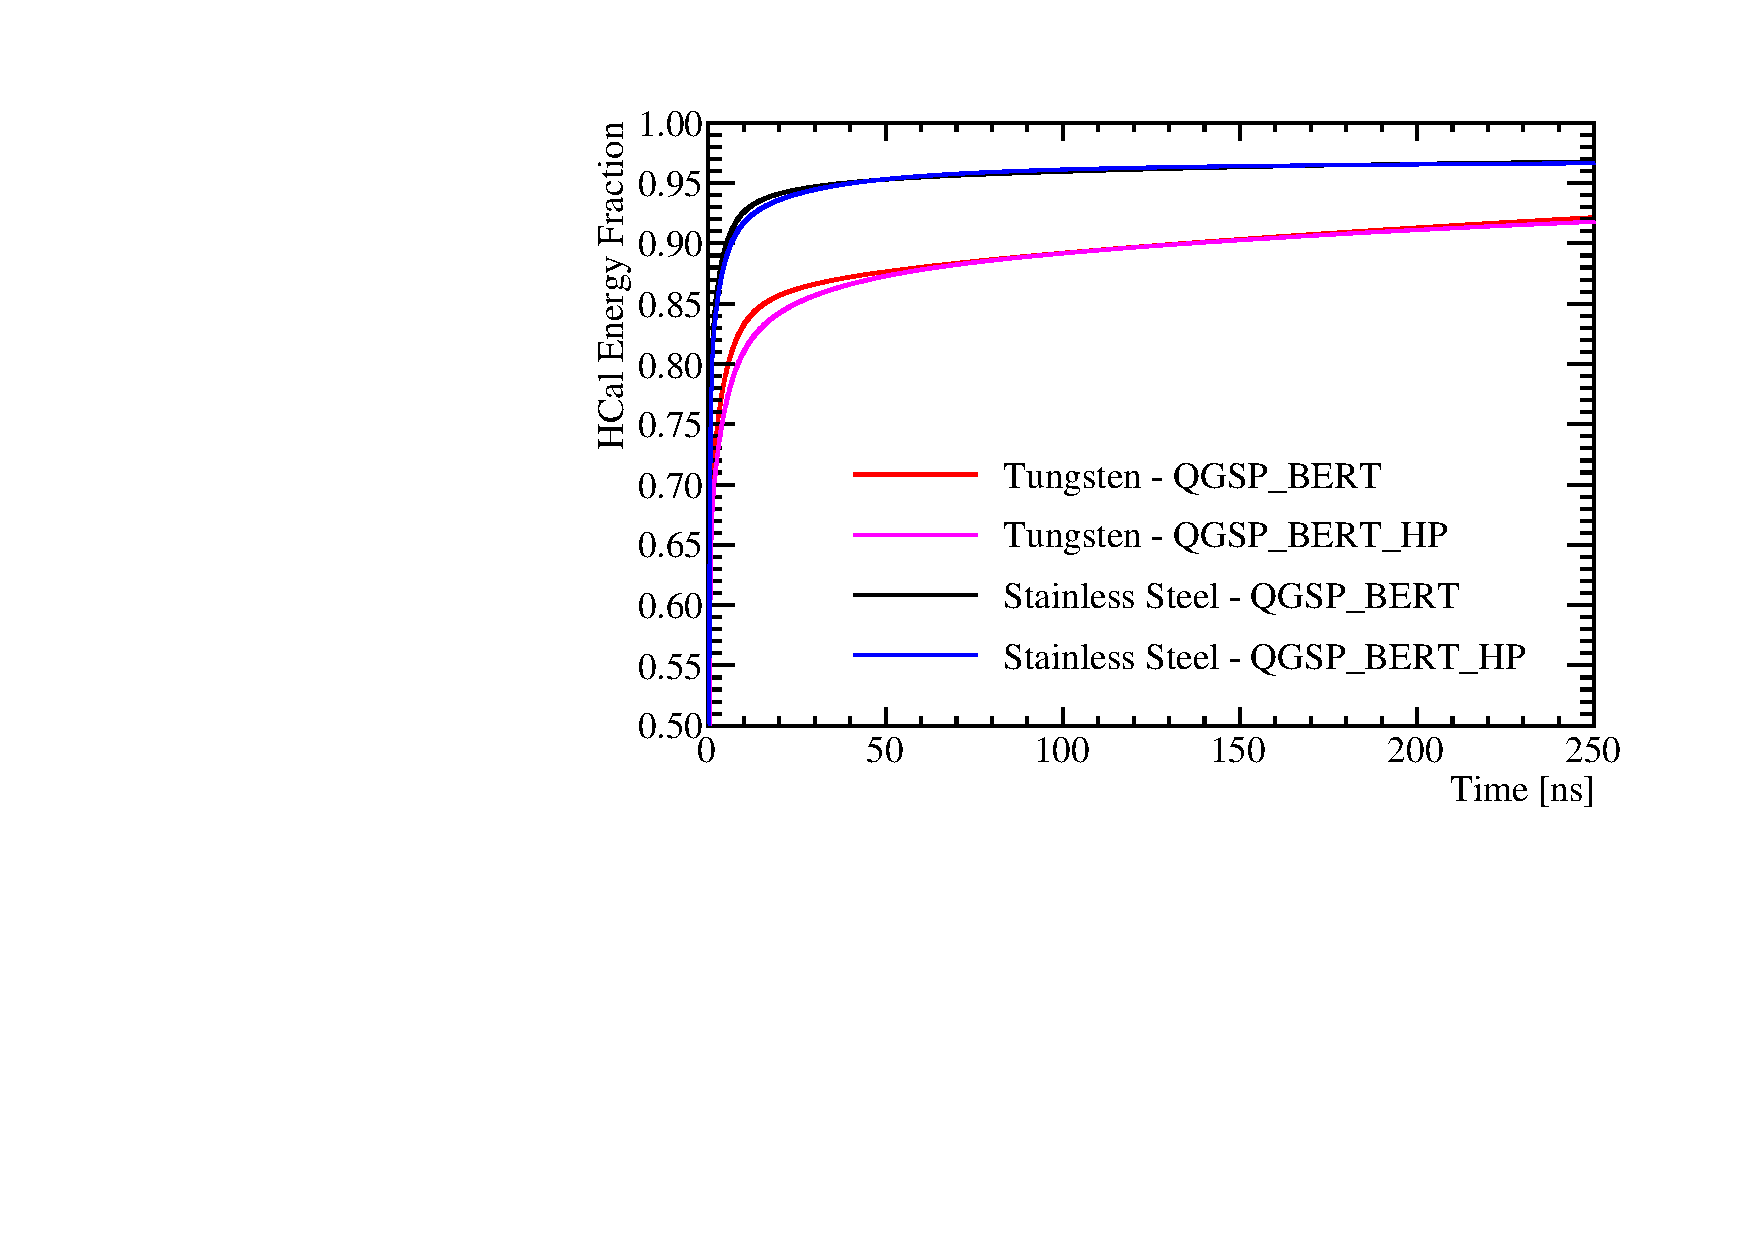
\includegraphics[width=0.5\textwidth]{OptimisationStudies/Plots/Description/HCalAbsorberMaterialTimings.pdf}
\caption[The fraction of the total calorimetric energy deposited in the HCal as a function of time for 25 GeV $\text{K}^{0}_{L}$ events using the steel and tungsten HCal options.  Results are shown for both the QGSP\_BERT and QGSP\_BERT\_HP physics lists.  The calorimeter hit times have been corrected for straight line time of flight to the impact point.]{The fraction of the total calorimetric energy deposited in the HCal as a function of time for 25 GeV $\text{K}^{0}_{L}$ events using the steel and tungsten HCal options.  Results are shown for both the QGSP\_BERT and QGSP\_BERT\_HP physics lists.  The calorimeter hit times have been corrected for straight line time of flight to the impact point.}
\label{fig:hcalabsmaterialtiming}
\end{figure} 

The energy resolution for 50 GeV $\text{K}^{0}_{L}$ events using the nominal ILD detector model with a stainless steel and tungsten HCal absorber material can be found in table \ref{table:erhcalabsmaterial}.  The tungsten HCal option offers a slight improvement over steel in the energy resolution for these samples.  This will be caused by differences in the atomic structure of the two materials, which will lead to different developments of the hadronic showers within them.  One example of this would be that energy losses to nuclear binding energies will be smaller in tungsten than steel (iron) as the atomic nuclei for tungsten is less stable and so less energy is needed to liberate nucleons in the shower development.  This will lead to a larger signal in the tungsten calorimeter and a reduction in the energy resolution in comparison to steel.  These results also indicated that the addition of the high precision neutron package did not alter the detector performance significantly for either option.  

\begin{table}[h!]
\centering
\begin{tabular}{ l l l }
\hline
HCal Option & Energy Resolution [\%] \\
\hline
Stainless Steel, QGSP\_BERT & $8.8\pm0.2$ \\
Stainless Steel, QGSP\_BERT\_HP & $9.0\pm0.3$ \\
Tungsten, QGSP\_BERT & $8.3\pm0.2$ \\
Tungsten, QGSP\_BERT\_HP & $8.3\pm0.2$ \\
\hline
\end{tabular}
\caption[The energy resolution using the nominal ILD detector with various HCal options determined using 50 GeV $\text{K}^{0}_{L}$ events.]{The energy resolution using the nominal ILD detector with various HCal options determined using 50 GeV $\text{K}^{0}_{L}$ events.}
\label{table:erhcalabsmaterial}
\end{table}

It should be emphasised that in determining these results, the HCal cell truncation, as described in chapter \ref{chap:energyestimators}, was separately tuned for the tungsten option.  This had to be done as the average cell energy is greater when using tungsten, as opposed to steel, for the HCal absorber material because tungsten has a larger number of radiation lengths per unit length than steel does.  As the HCal primarily measures hadronic showers one may naively expect the number of radiation lengths in the HCal to be irrelevant to performance, given both options have the same number of nuclear interaction lengths, but this is not the case as all hadronic showers have an electromagnetic component, from the decays of $\pi^{0}\rightarrow \gamma \gamma$.  Therefore, these shower components deposit more energy per unit length in the HCal, which raises the average cell energy.  

The jet energy resolutions for various jet energies are shown in table \ref{table:jerhcalabsmaterial} for the various HCal options considered.  These results indicate that steel outperforms tungsten as the absorber material for the HCal.  Furthermore, as the jet energy increases, the magnitude of the difference in jet energy resolutions between the two options grows.  This indicates the differences in jet energy resolution between the two options is driven by the confusion contribution since this contribution grows with increasing jet energy.  Furthermore, as the $\text{K}^{0}_{L}$ energy resolution was only slightly better for the tungsten option it is expected that the intrinsic energy resolution contribution to the jet energy resolution will not vary significantly between the two as only a small fraction of jet energy is measured in the HCal.  The intrinsic energy resolution and confusion contributions to the jet energy resolution for 45 and 250 GeV jets are shown in table \ref{table:jerbdhcalabsmaterial}.  As expected, the intrinsic energy resolution contribution to the jet energy resolution is nearly identical between the various options.  The confusion contribution to the jet energy resolution is larger for the tungsten HCal option than for the steel HCal option.  This will be due to the PandoraPFA algorithms being tuned for HCal cell dimensions for the steel HCal option, while the cells for the tungsten option are thinner by a factor of approximately $\frac{\lambda_{I}^{Steel}}{\lambda_{I}^{Tungsten}} \approx 1.7$, where $\lambda_{I}^{x}$ is the distance of one radiation length in material $x$.  It is unfeasible to tune all of the PandoraPFA algorithms to each detector geometry, however, the breakdowns of the jet energy resolution indicate that even if it were possible to obtain the same confusion contributions for both options, the tungsten option would offer no advantage to the steel option in terms of the intrinsic jet energy resolution.  Once again, it was noted that the use of the QGSP\_BERT\_HP physics list, as opposed to QGSP\_BERT, made a minimal impact on these results.

\begin{table}[h!]
\centering
\begin{tabular}{ l l l l l }
\hline
HCal Option & Jet Energy & & & \\
 & Resolution & & & \\
 & [\%] & & & \\
 & 45 GeV & 100 GeV & 180 GeV & 250 GeV \\
\hline
Stainless Steel, QGSP\_BERT & $3.65 \pm 0.05$ &$2.88 \pm 0.04$ &$2.85 \pm 0.04$ &$2.97 \pm 0.05$ \\
Stainless Steel, QGSP\_BERT\_HP & $3.67 \pm 0.05$ &$2.92 \pm 0.04$ &$2.86 \pm 0.04$ &$3.03 \pm 0.04$ \\
Tungsten, QGSP\_BERT & $3.78 \pm 0.05$ & $3.12 \pm 0.04$ & $3.15 \pm 0.04$ & $3.43 \pm 0.04 |$ \\
Tungsten, QGSP\_BERT\_HP & $3.80 \pm 0.05$ & $3.08 \pm 0.04$ & $3.24 \pm 0.04$ & $3.41 \pm 0.04$ \\
%Tungsten, QGSP\_BERT & $3.67 \pm 0.05$ &$3.12 \pm 0.04$ &$3.36 \pm 0.04$ &$3.76 \pm 0.05$ \\ 1 GeV Truncation 
%Tungsten, QGSP\_BERT\_HP & $3.69 \pm 0.05$ &$3.03 \pm 0.04$ &$3.38 \pm 0.04$ &$3.80 \pm 0.05$ \\ 1 GeV Truncation
\hline
\end{tabular}
\caption[The jet energy resolution using the nominal ILD detector with various HCal options for various jet energies.]{The jet energy resolution using the nominal ILD detector with various HCal options for various jet energies.}
\label{table:jerhcalabsmaterial}
\end{table}

\begin{table}[h!]
\centering
\begin{tabular}{ l l l l l }
\hline
HCal Option & Jet Energy & & & \\
 & Resolution & & & \\
 & [\%] & & & \\
 & 45 GeV & & 250 GeV & \\
 & Intrinsic & Confusion & Intrinsic & Confusion \\
\hline
Stainless Steel, QGSP\_BERT & $2.93 \pm 0.04$ & $2.16 \pm 0.06$ & $1.69 \pm 0.02$ &$2.45 \pm 0.05$ \\
Stainless Steel, QGSP\_BERT\_HP & $2.98 \pm 0.04$ &$2.15 \pm 0.06$ &$1.65 \pm 0.02$ &$2.53 \pm 0.04$ \\
Tungsten, QGSP\_BERT & $2.97 \pm 0.04$ & $2.34 \pm 0.06$ & $1.65 \pm 0.02$ & $3.01 \pm 0.05$ \\
Tungsten, QGSP\_BERT\_HP & $2.92 \pm 0.04$ & $2.42 \pm 0.06$ & $1.65 \pm 0.02$ & $2.99 \pm 0.05$ \\
\hline
\end{tabular}
\caption[The contributions to the jet energy resolution using the nominal ILD detector with various HCal options for 45 and 250 GeV jet energies.]{The contributions to the jet energy resolution using the nominal ILD detector with various HCal options for 45 and 250 GeV jet energies.}
\label{table:jerbdhcalabsmaterial}
\end{table}

In conclusion, there are no large differences in the intrinsic energy resolution of the ILD detector simulation, for either neutral hadrons or jets, when changing the HCal absorber material from steel to tungsten.  The steel option HCal outperforms the tungsten option in terms of pattern recognition confusion, when using the default PandoraPFA settings, although this could be addressed should it become clear that tungsten were a preferred option.  However, when examining the mechanical properties of steel and tungsten, it is clear that steel has a significant advantage over tungsten in terms of rigidity \cite{Linssen:2012hp}.  This means that fewer support structures would be required for the calorimeter leading to less dead material and better performance, which makes steel the more preferred option of the two.

%========================================================================================
%========================================================================================

\section{Global Detector Parameters}
The detector geometry and the magnetic field strength are major cost drivers for the detector.  Both will affect the jet energy resolution and, for completeness, are considered here.  

%========================================================================================

\subsection{The Magnetic Field Strength}
\label{sec:bfield}
In the particle flow paradigm the momentum of charged particles is obtained through the curvature of the track they traverse as they bend in the magnetic field.  Therefore, the magnetic field is an integral element for the successful application of particle flow calorimetry.  Furthermore, the magnetic field deflects charged particles away from neutral ones in jets.  The stronger the magnetic field, the larger the separation between the calorimetric energy deposits made by charged and neutral particles from jets.  This, in turn, makes it easier to associate charged particle tracks to the correct calorimetric energy deposits.  Therefore, it is expected that a stronger magnetic field will lead to better jet energy resolutions through a reduction of the confusion contribution to the jet energy resolution.  

Detector models were simulated where the magnetic field was varied from 1 to 5~T in steps of 0.5~T and the jet energy resolutions for these detectors is shown in figure \ref{fig:bfield}.  For high energy jets there is a strong trend whereby a stronger magnetic field lead to a better jet energy resolution.  On the other hand, at low jet energies the jet energy resolution is almost invariant to changes in the magnetic field.  

The jet energy resolution breakdowns into the various contributions are shown in figure \ref{fig:bfieldbreak} and as expected there is clear reduction in the confusion contribution to the jet energy resolution with increasing magnetic field strength.  Furthermore, there is a reduction in intrinsic energy resolution with increasing magnetic field strength for low energy jets.  At low energies, the radius of curvature of the helix charged particles traverse will be small.  If the radius for a given particle is small enough, it will not make it into the calorimeters.  In this case, only if the track produced from this particle passes tight selection cuts, designed to ensure the track originates from the IP, will the track be used in the reconstruction.  Therefore, energy can and will be lost from events where particles are stuck within the tracker.  Given the radii of curvature is inversely proportional to the magnetic field strength, the larger the magnetic field strength the more tracks will be confined to the tracker as is shown by figure \ref{fig:bfieldchargedparticles}.  The more tracks that are confined to the tracker, the worse the intrinsic energy resolution becomes as inevitably some tracks fail the quality cuts.  At high jet energies, low transverse momentum charged particles will still get trapped within the tracker, however, these contribute fractionally little energy to the total reconstructed energy.  Therefore, the trend of worsening intrinsic energy resolution with increasing magnetic field strength is less pronounced as the jet energy grows.  At very low magnetic field strengths and high jet energies, the intrinsic energy resolution actually degrades, due to an artefact in the determination of the intrinsic energy resolution.  The intrinsic energy resolution is determined by associating a single MC particle to each calorimeter cell.  At low magnetic field strengths and high jet energies, many of the MC particles will have overlapping energy deposits wihtin the calorimeter cells and so associating a single MC particle per cell is inaccurate.  This leads to imperfect association of charged particle tracks to calorimetric energy deposits, which worsens the intrinsic energy resolution.  However, as this effect is second order small in comparison to changes in the confusion contribution the overall dependancy of detector performance on the magnetic field strength can be confidently quantified.  

\begin{figure}[h!]
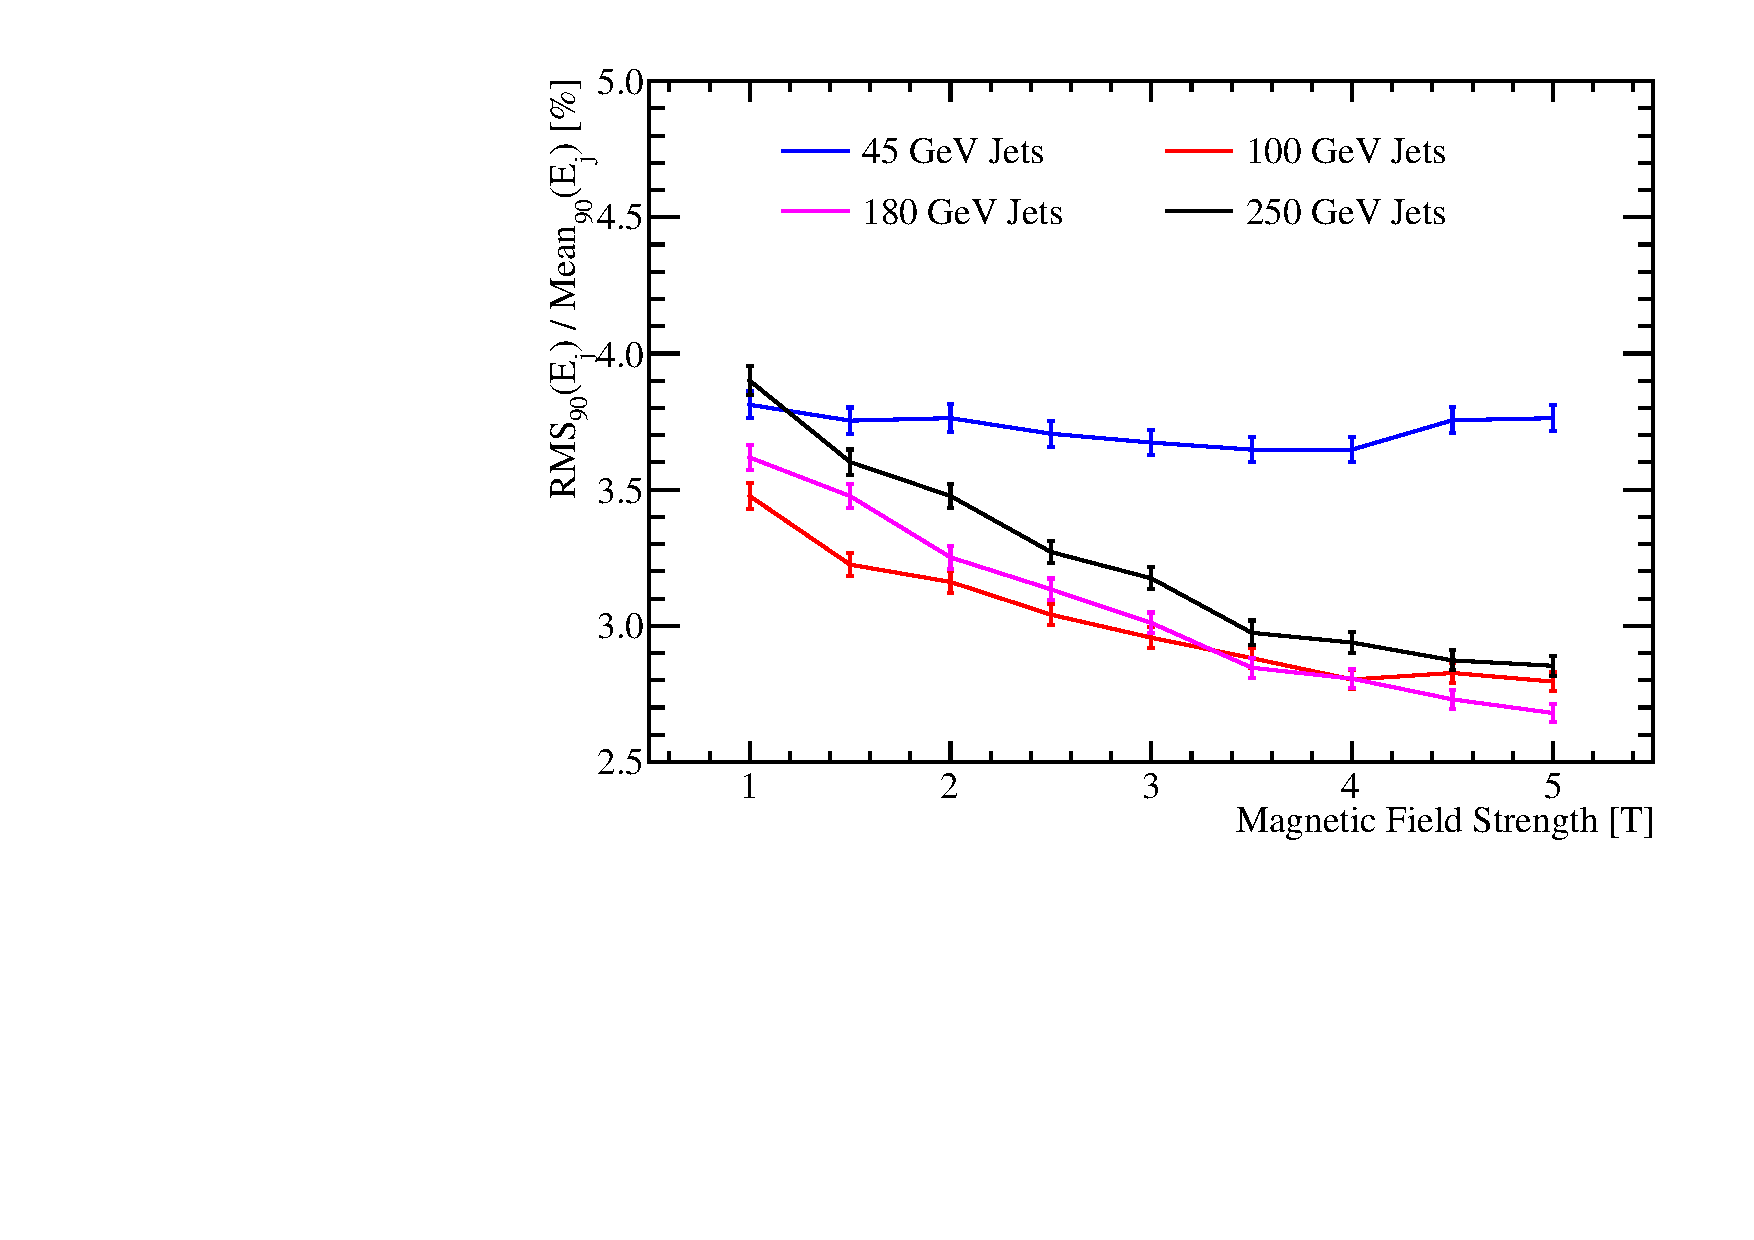
\includegraphics[width=0.5\textwidth]{OptimisationStudies/Plots/JetEnergyResolutions/JER_vs_MagneticFieldStrength.pdf}
\caption[The jet energy resolution using the nominal ILD detector as a function of the magnetic field strength for various jet energies.]{The jet energy resolution using the nominal ILD detector as a function of the magnetic field strength for various jet energies.}
\label{fig:bfield}
\end{figure}

\begin{figure}[h!]
\subfloat[]{\label{fig:bfield45break}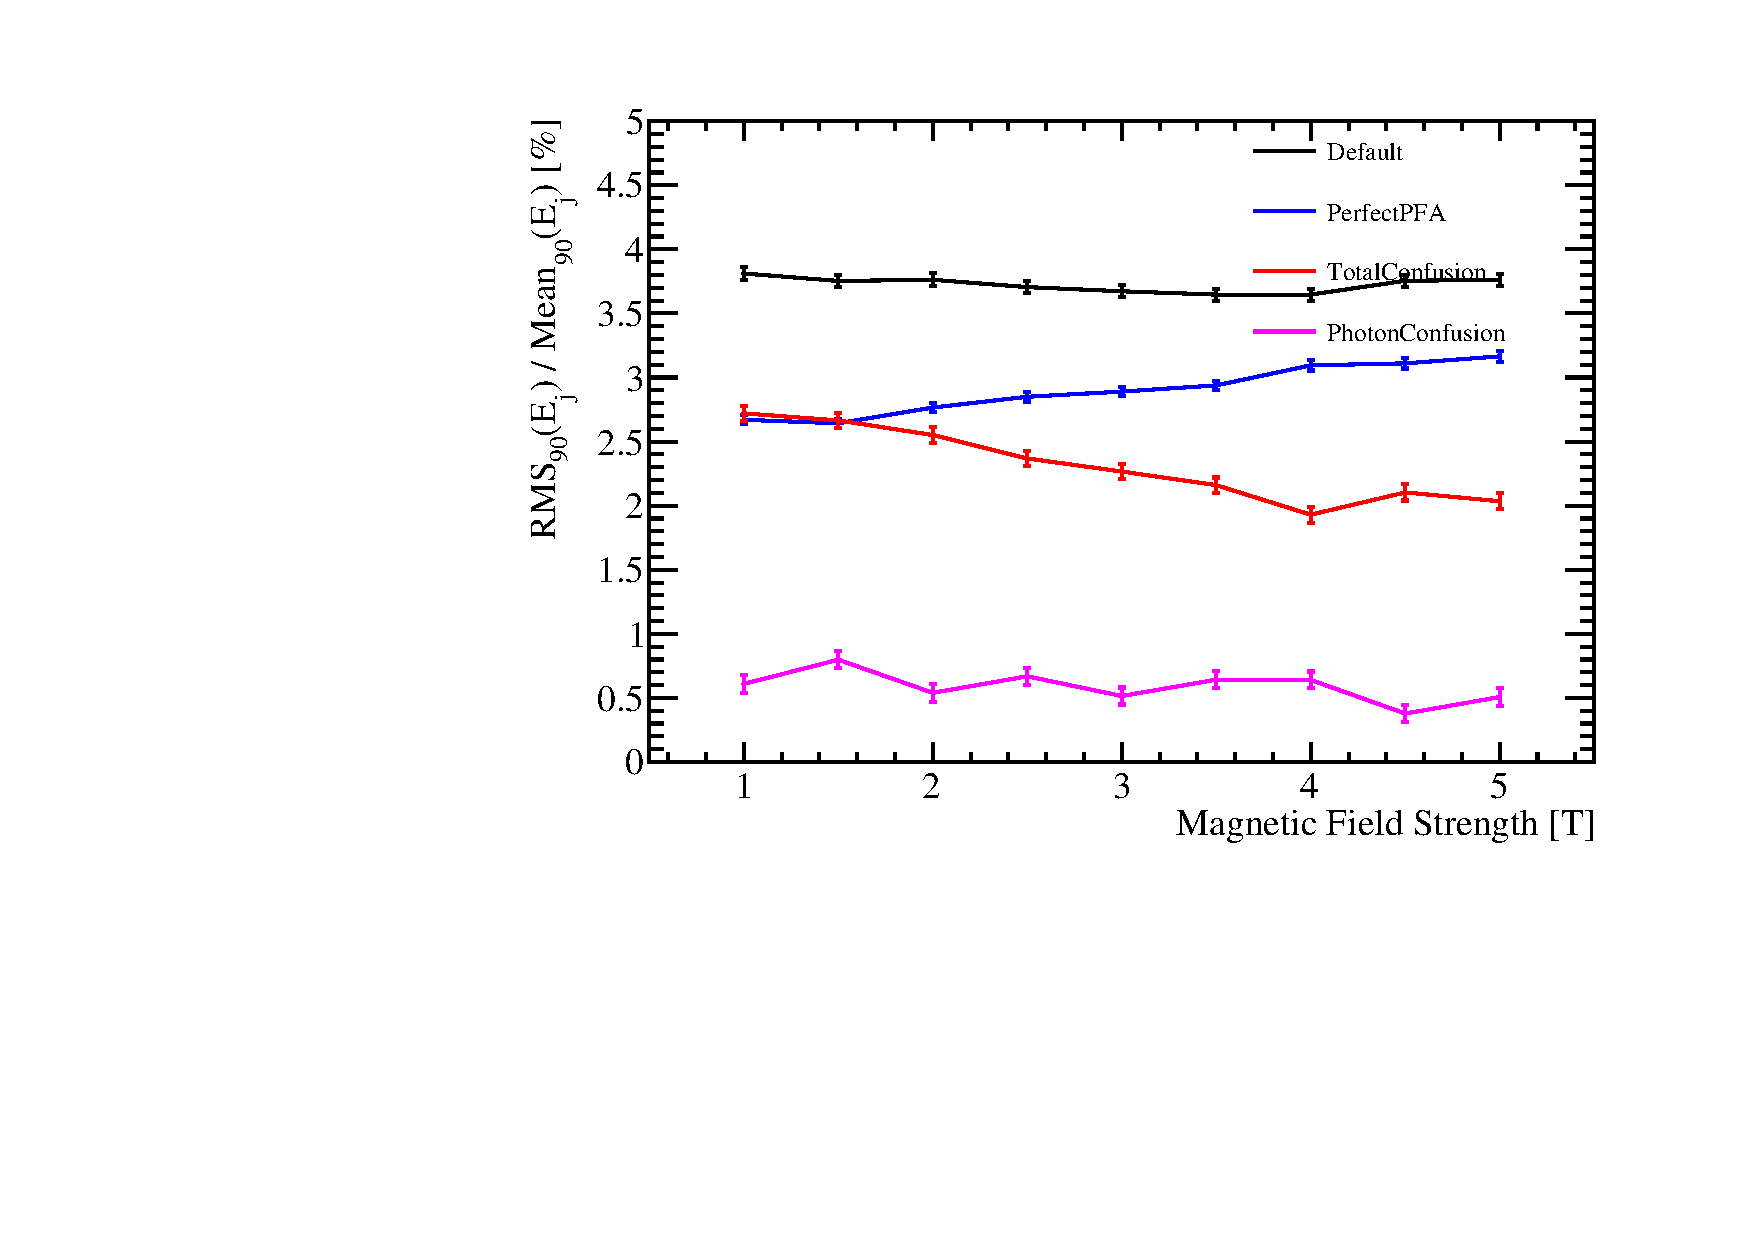
\includegraphics[width=0.5\textwidth]{OptimisationStudies/Plots/JetEnergyResolutions/JER_vs_MagneticFieldStrength_91GeV_DiJet_Breakdown.pdf}}
\subfloat[]{\label{fig:bfield250break}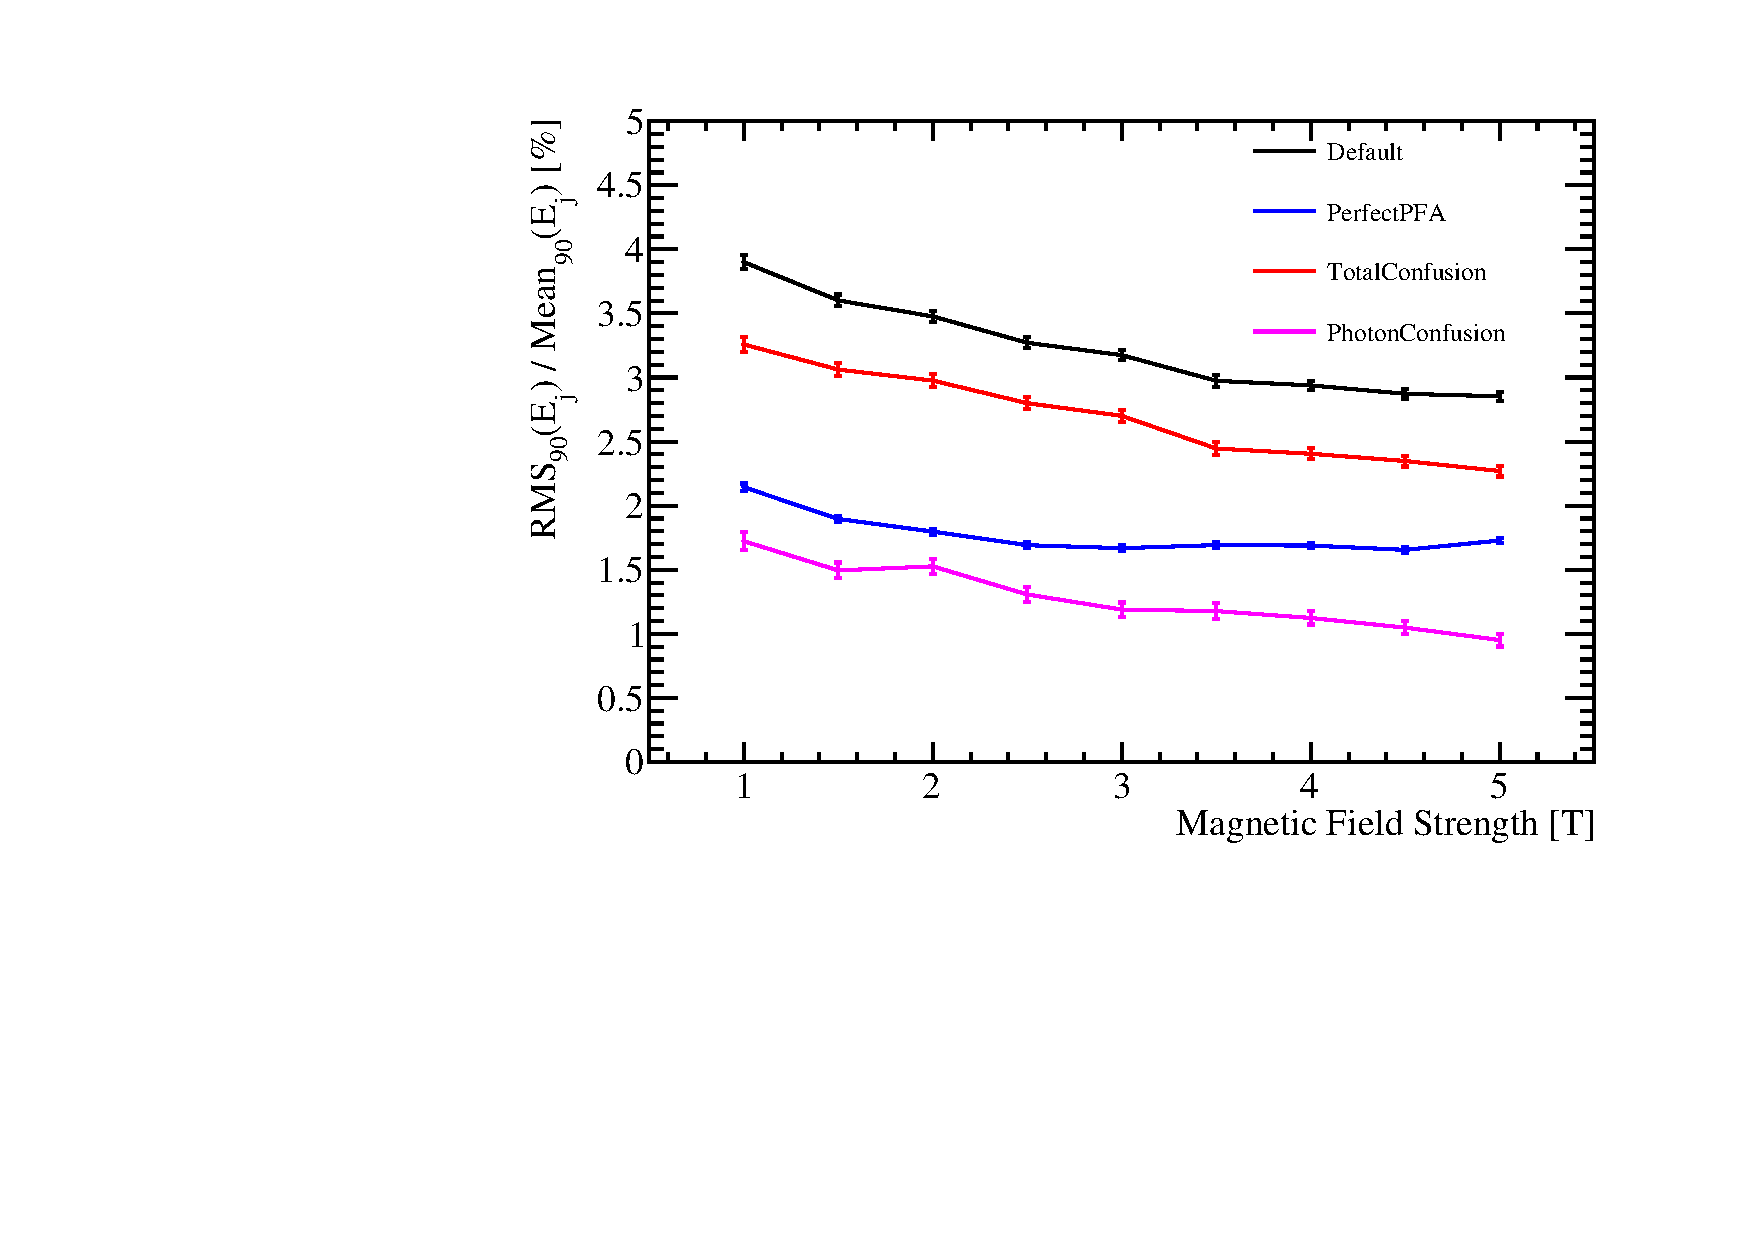
\includegraphics[width=0.5\textwidth]{OptimisationStudies/Plots/JetEnergyResolutions/JER_vs_MagneticFieldStrength_500GeV_DiJet_Breakdown.pdf}}
\caption[The contributions to the jet energy resolution as a function of the magnetic field strength using the nominal ILD detector model for \protect\subref{fig:bfield45break} 45 GeV jets and \protect\subref{fig:bfield250break} 250 GeV jets.  The black curves correspond to the standard reconstruction, the blue curves to the intrinsic energy resolution contribution to the jet energy resolution, the red curves to the confusion contribution to the jet energy resolution and the magenta curves to the confusion contribution to the jet energy resolution related solely to $\gamma$ reconstruction.]{The contributions to the jet energy resolution as a function of the magnetic field strength using the nominal ILD detector model for \protect\subref{fig:bfield45break} 45 GeV jets and \protect\subref{fig:bfield250break} 250 GeV jets.  The black curves correspond to the standard reconstruction, the blue curves to the intrinsic energy resolution contribution to the jet energy resolution, the red curves to the confusion contribution to the jet energy resolution and the magenta curves to the confusion contribution to the jet energy resolution related solely to $\gamma$ reconstruction.}
\label{fig:bfieldbreak}
\end{figure}

\begin{figure}[h!]
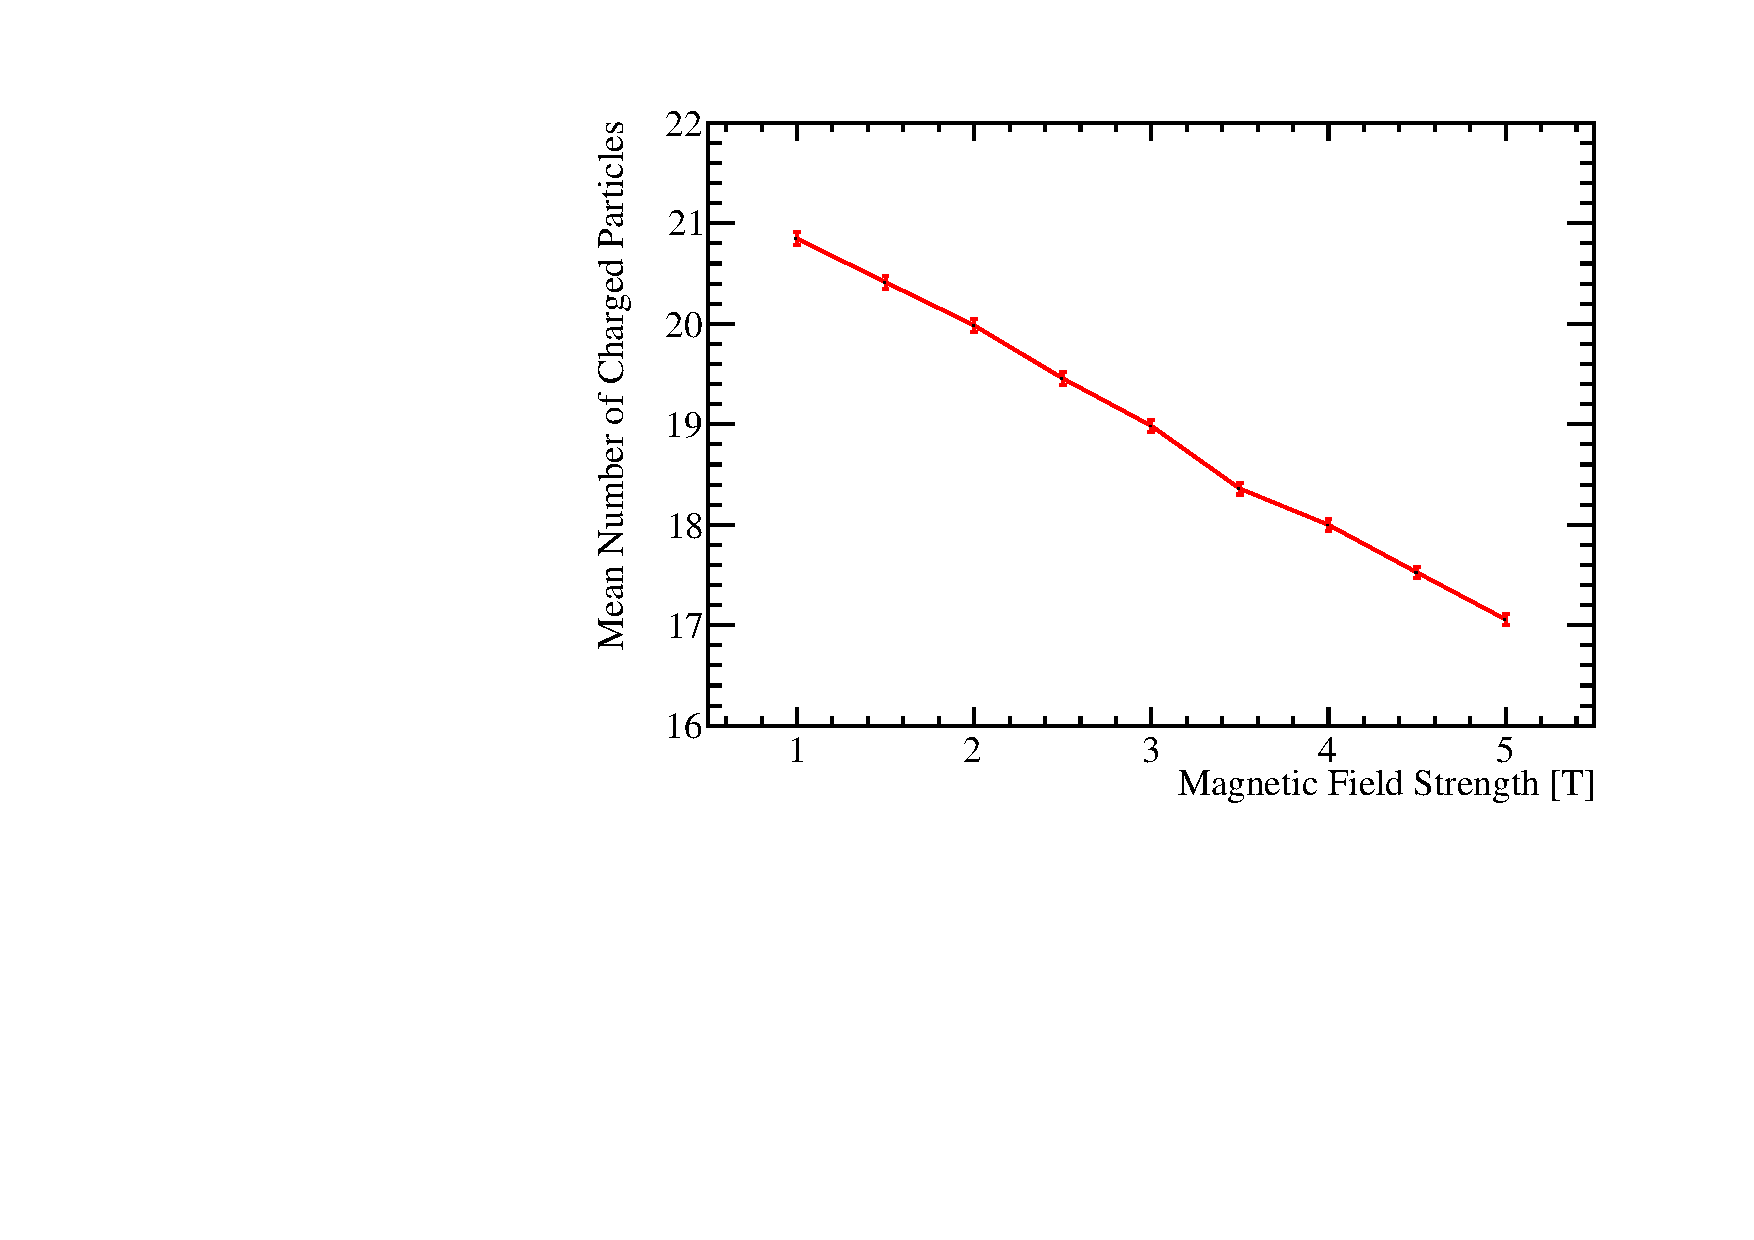
\includegraphics[width=0.5\textwidth]{OptimisationStudies/Plots/Description/BField/BFieldNumbers_91GeV_Z_uds.pdf}
\caption[The mean number of reconstructed charged particles as a function of the magnetic field strength for 91 GeV Z$\rightarrow$uds di-jet events.  The nominal ILD detector model was used and the pattern recognition has been fully cheated using the MC information.]{The mean number of reconstructed charged particles as a function of the magnetic field strength for 91 GeV Z$\rightarrow$uds di-jet events.  The nominal ILD detector model was used and the pattern recognition has been fully cheated using the MC information.}
\label{fig:bfieldchargedparticles}
\end{figure}

In summary, increasing the magnetic field strength is beneficial to detector performance as it reduces confusion from associating tracks to calorimetric energy deposits from charged particles.  While there is a reduction in the intrinsic energy resolution for low transverse momentum jets with increasing magnetic field strength, this effect is largely offset by the change in confusion.  While the nominal field of 3.5 T gives good performance increasing the field strength is a clear way of making gains in detector performance.

%========================================================================================

\subsection{Inner ECal Radius}
Detector models were considered where the ECal inner radius was set to 1208, 1408, 1608, 1808 (nominal) and 2008~mm.  All other detector parameters are identical to those found in the nominal ILD detector model.

Figure \ref{fig:ecalinnerr} shows the dependence of the jet energy resolution on the ECal inner radius.  The simulations indicate that a large ECal inner radius was highly beneficial to detector performance, which is due to the increase in the time it takes for particles to reach the calorimeters.  The longer it takes for the particles to reach the calorimeters the more the charged particles will bend and the larger separation between calorimetric energy deposits from charged and neutral particles.  This larger separation reduces the confusion when associating calorimetric energy deposits to tracks and so improves the detector performance.  This conclusion is backed up by the decomposition of the jet energy resolution for the low and high energy jets, shown in figure \ref{fig:ecalinnerrbreak}, which explicitly show a reduction in confusion with increasing ECal inner radius.  The intrinsic energy resolution of the detectors showed no strong dependence on the inner ECal radius.  There is a small degradation in intrinsic energy resolution at low ECal inner radii due to the association of a single MC particle per calorimeter cell when running the cheated pattern recognition as explained in section \ref{sec:bfield}.  Again, this effect has little bearing on the final conclusions as the change in intrinsic energy resolution across the detector models is a second order effect.  

\begin{figure}[h!]
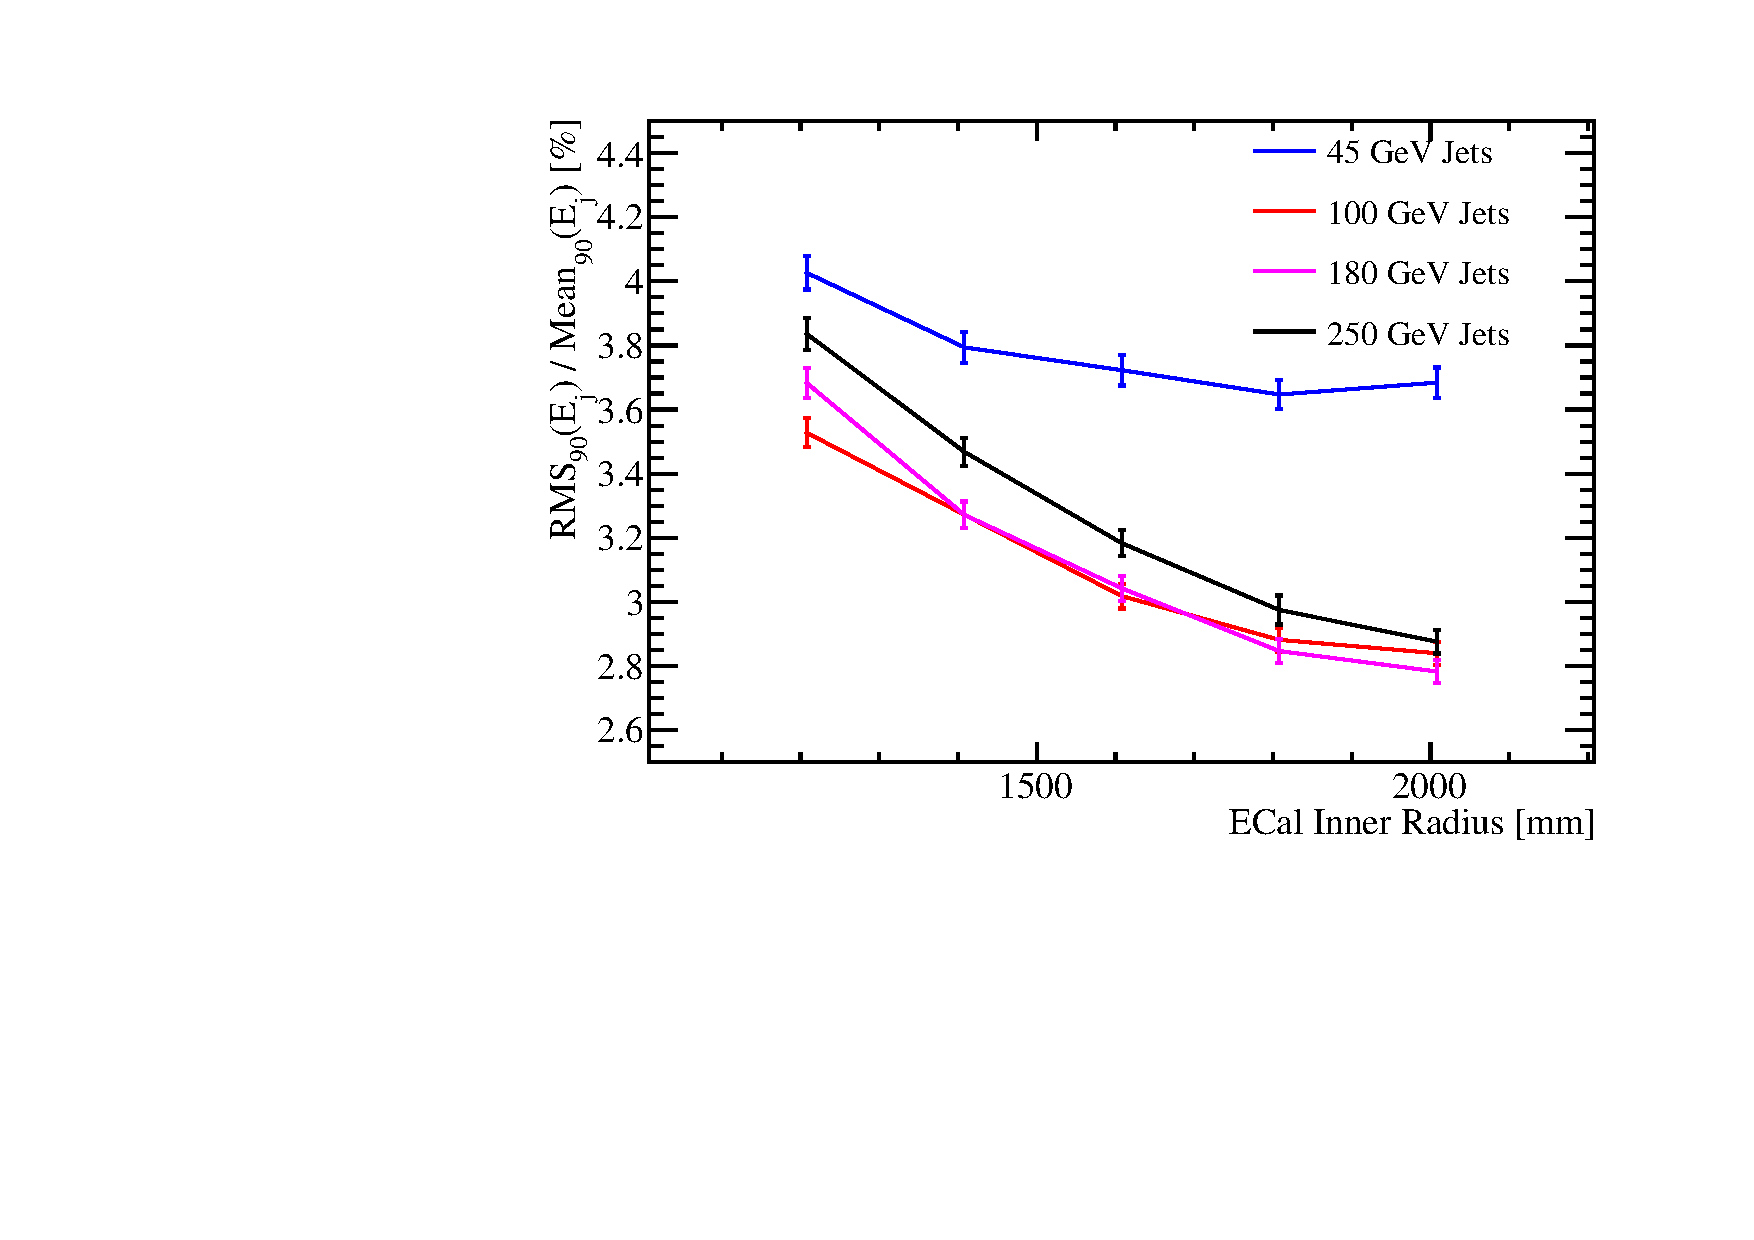
\includegraphics[width=0.5\textwidth]{OptimisationStudies/Plots/JetEnergyResolutions/JER_vs_ECalInnerRadius.pdf}
\caption[The jet energy resolution using the nominal ILD detector as a function of the ECal inner radius for various jet energies.]{The jet energy resolution using the nominal ILD detector as a function of the ECal inner radius for various jet energies.}
\label{fig:ecalinnerr}
\end{figure}

\begin{figure}[h!]
\subfloat[]{\label{fig:ecalinnerr45break}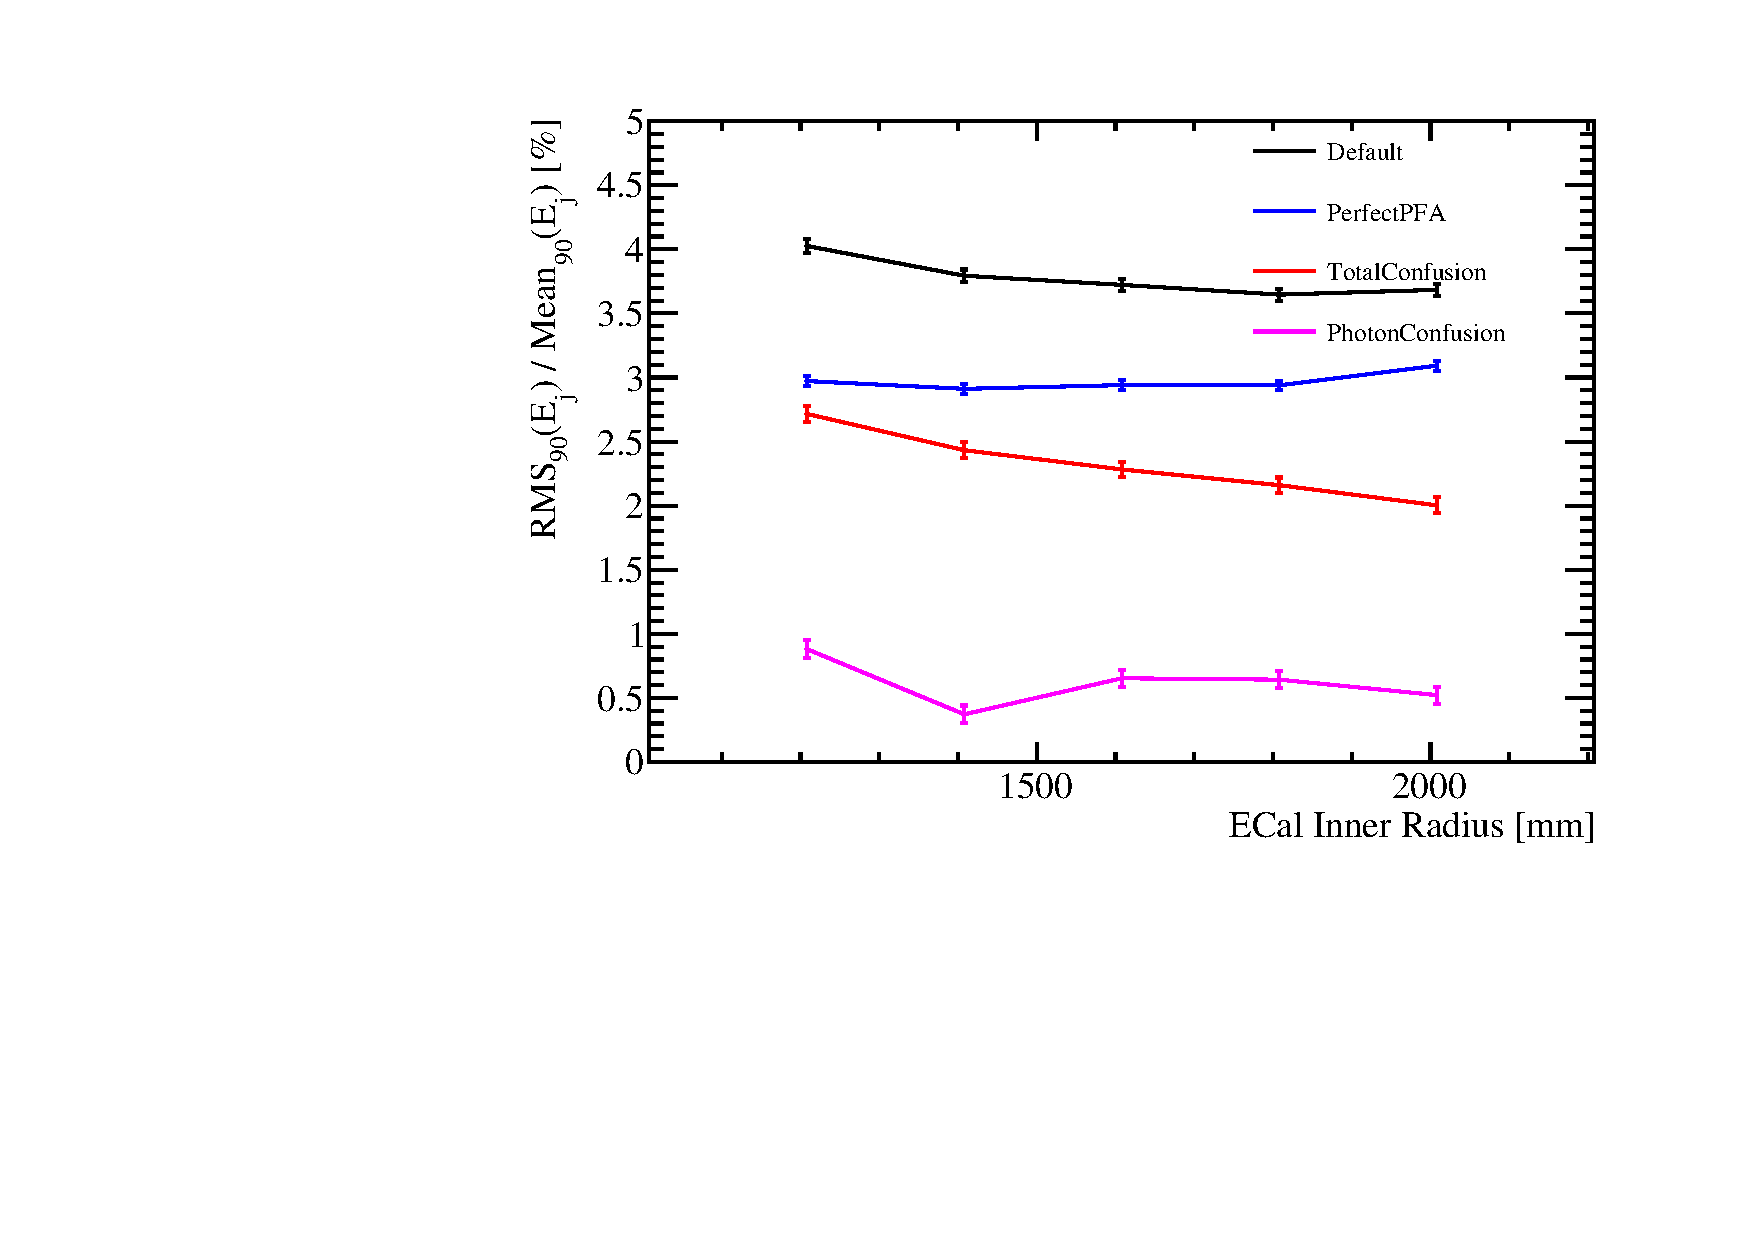
\includegraphics[width=0.5\textwidth]{OptimisationStudies/Plots/JetEnergyResolutions/JER_vs_ECalInnerRadius_91GeV_DiJet_Breakdown.pdf}}
\subfloat[]{\label{fig:ecalinnerr250break}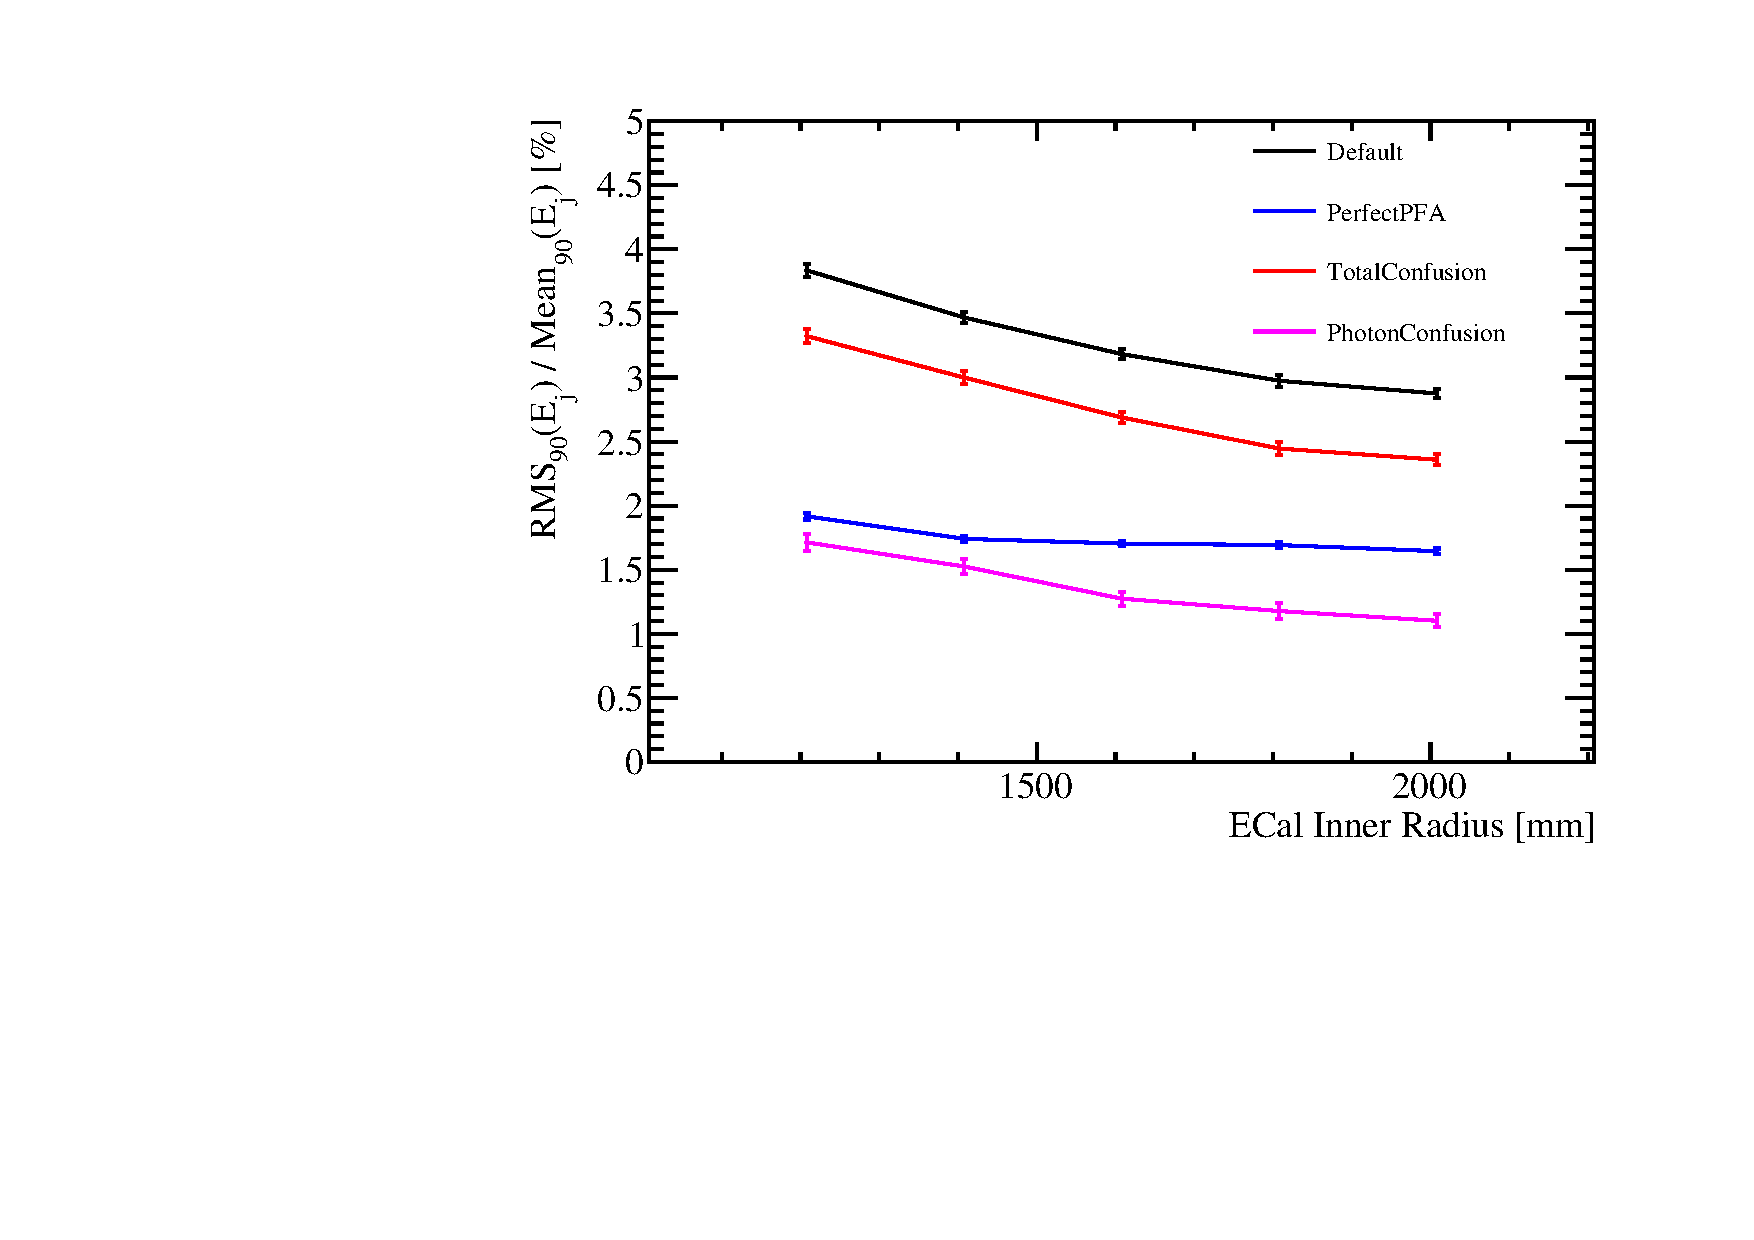
\includegraphics[width=0.5\textwidth]{OptimisationStudies/Plots/JetEnergyResolutions/JER_vs_ECalInnerRadius_500GeV_DiJet_Breakdown.pdf}}
\caption[The contributions to the jet energy resolution as a function of the ECal inner radius using the nominal ILD detector model for \protect\subref{fig:ecalinnerr45break} 45 GeV jets and \protect\subref{fig:ecalinnerr250break} 250 GeV jets.  The black curves correspond to the standard reconstruction, the blue curves to the intrinsic energy resolution contribution to the jet energy resolution, the red curves to the confusion contribution to the jet energy resolution and the magenta curves to the confusion contribution to the jet energy resolution related solely to $\gamma$ reconstruction.]{The contributions to the jet energy resolution as a function of the ECal inner radius using the nominal ILD detector model for \protect\subref{fig:ecalinnerr45break} 45 GeV jets and \protect\subref{fig:ecalinnerr250break} 250 GeV jets.  The black curves correspond to the standard reconstruction, the blue curves to the intrinsic energy resolution contribution to the jet energy resolution, the red curves to the confusion contribution to the jet energy resolution and the magenta curves to the confusion contribution to the jet energy resolution related solely to $\gamma$ reconstruction.}
\label{fig:ecalinnerrbreak}
\end{figure}

In conclusion, increasing the ECal inner radius benefits the jet energy resolution significantly.  This trend is driven by changes to the confusion in associating calorimetric energy deposits to charged particle tracks, with a larger ECal inner radius producing a reduction in the confusion as separation of charged and neutral particle energy deposits increases.  
